%%%%%%%%%%%%%%%%%%%%%%%%%%%%%%%%%%%%%%%%%%%%%%%%%
%
%	MSc THESIS TEMPLATE
%	developed for my master thesis at the Universitá di Torino
%
%	by Eugenio Senes (eugenio.senes@gmail.com)
%
%	released under MIT license, so share, modify and enjoy, but quoting the author !
%
%%%%%%%%%%%%%%%%%%%%%%%%%%%%%%%%%%%%%%%%%%%%%%%%%

%% DOCUMENT CLASS (alternative to book is 'report')
% Print just right page or both sides (comment the other one)
%\documentclass[12pt,a4paper,openright,oneside]{book}	%%One sided
%\documentclass[12pt,a4paper,openright,twoside]{book}	%%Double sided
\documentclass[12pt,a4paper,oneside]{book}

%% SET MARGINS OF THE PAGES
\usepackage[a4paper,portrait, left=35mm, right=20mm, top=35mm, bottom=30mm]{geometry}

%% HEADERS AND FOOTERS
\usepackage{fancyhdr}
\pagestyle{fancy}
\fancyhf{} 			%clears default header and footer
%\fancyhead[RO]{\leftmark}
%\fancyhead[LE]{\leftmark}
%\fancyfoot[RO]{\thepage}
%\fancyfoot[LE]{\thepage}
\rhead{} 			%right head
\lhead{} 	%left head
\rfoot{\thepage}
%%consider using also chead, cfoot, lfoot
%coherce the plain stile to this (e.g. the first page of every chapter)
\fancypagestyle{plain}{
	\fancyhf{}
	\rfoot{\thepage}
	\renewcommand{\headrulewidth}{0pt}
	\renewcommand{\footrulewidth}{0pt}
}

%% CLEAR PAGE WITHOUT NUMBER AT THE BEGINNING OF CHAPTERS
\let\origdoublepage\cleardoublepage
\newcommand{\clearemptydoublepage}{%
  \clearpage
  {\pagestyle{empty}\origdoublepage}%
}
%% ALLOW PAGE ROTATION
\usepackage{lscape}

%% HYPERTEXT SETUP
\usepackage[unicode=true]{hyperref}
\hypersetup{
	pdfauthor={Filippo Valle},
	pdftitle={MSc thesis},
	pdfsubject={Topic Modelling},
	pdfkeywords={network-theory, graph-theory, topic-modelling, machine-learning, clustering},
	breaklinks=true,
	colorlinks=true,
	citecolor=blue,
	urlcolor=blue,
	linkcolor=black
}

\author{Filippo Valle}
\date{\today}
\title{A topic model approach reveals hidden structures in datasets of healthy and cancer tissues.}

%% FONTS AND SYMBOLS
\usepackage[utf8]{inputenc}	%%input font setting
\usepackage{textcomp}
\usepackage[T1]{fontenc} 		%%font for automatic recognition of letters with the accent
\usepackage{amsfonts}		%%fonts for the mathematical rendering of formulas
\usepackage{amssymb}
\usepackage{amsmath}
%% CHAPTERS STRUCTURE
\usepackage[english]{babel} %%Set English as main language of the document
%% FIGURES
\usepackage{graphicx}
%% TABLES
\usepackage{booktabs}		%%allow use of \toprule, \midrule, \bottomrule in tables
%%CAPTIONS
\usepackage{caption}
%% CODE LISTINGS
\usepackage{listings}		%%allow to use code listings
\usepackage{rotating}  %%sideways/
\usepackage{placeins}  %%\FloatBarrier
\usepackage{float} %force [htb] enabling [H]
\usepackage{color}
\usepackage{url}

\lstdefinestyle{myPython}{
backgroundcolor=\color{white},   % choose the background color; you must add \usepackage{color} or \usepackage{xcolor}; should come as last argument
basicstyle=\footnotesize\ttfamily,        % the size of the fonts that are used for the code
breakatwhitespace=false,         % sets if automatic breaks should only happen at whitespace
breaklines=true,                 % sets automatic line breaking
captionpos=b,                    % sets the caption-position to bottom
commentstyle=\color{mygray},    % comment style
keepspaces=true,                 % keeps spaces in text, useful for keeping indentation of code (possibly needs columns=flexible)
keywordstyle=\color{mygreen},       % keyword style
identifierstyle=\color{black},
language=python,                 % the language of the code
morekeywords={*, as},
numbers=left,                    % where to put the line-numbers; possible values are (none, left, right)
numbersep=5pt,                   % how far the line-numbers are from the code
numberstyle=\tiny\color{mygray}, % the style that is used for the line-numbers
rulecolor=\color{black},         % if not set, the frame-color may be changed on line-breaks within not-black text (e.g. comments (green here))
showspaces=false,                % show spaces everywhere adding particular underscores; it overrides 'showstringspaces'
showstringspaces=false,          % underline spaces within strings only
showtabs=false,                  % show tabs within strings adding particular underscores
stepnumber=2,                    % the step between two line-numbers. If it's 1, each line will be numbered
stringstyle=\color{myblue},     % string literal style
tabsize=2,	                   % sets default tabsize to 2 spaces
}


\definecolor{mygreen}{rgb}{0,0.6,0}
\definecolor{mygray}{rgb}{0.5,0.5,0.5}
\definecolor{mymauve}{rgb}{0.58,0,0.82}
\definecolor{myblue}{rgb}{0.44,0.62,0.78}
\definecolor{pythonred}{RGB}{255,0,0}
\definecolor{pythongreen}{RGB}{0,150,57}
\definecolor{pythonblue}{RGB}{58,0,242}
\definecolor{pythonorange}{RGB}{255,122,0}
\definecolor{pythonyellow}{RGB}{250,255,0}

%% HYPENATON
\hyphenation{te-si}	%manual hyphenation

%%commands
\newcommand{\avg}[1]{\left\langle #1\right\rangle}
\newcommand{\var}[1]{\sigma^2_{#1}}
\newcommand{\draft}[1]{\textcolor{red}{#1}}

%%%%%%%%%%%%%%%%%%%%%%%%%%%%%%%%%%%%%%%%%%%%%%%%%
%%%% BEGIN DOCUMENT
\begin{document}
%%%%%% HEAD  OF THE DOCUMENT
\frontmatter
%%FRONT PAGE
%\begin{titlepage}
%upper part
\begin{center}
{{\Large{\textsc{Universit\`a degli studi di Torino \\}}}} \vspace{5mm} {\small{\bf SCUOLA DI SCIENZE DELLA NATURA\\ \vspace{3mm}
Corso di Laurea Magistrale in Fisica dei Sistemi Complessi}}
\vspace{5mm}
\end{center}
%logo
\begin{center}

\includegraphics[scale=.3]{head/logo.png}
\end{center}
%title
\begin{center}
\vspace{5mm}
{\large{\bf Tesi di Laurea Magistrale\\}}
\vspace{5mm}
{\LARGE{\bf THE FANCY TITLE\\ OF MY FANCY THESIS\\}}
%\vspace{5mm}
%{\LARGE{\bf SECOND ROW TITLE}}
\end{center}
\vspace{20mm}
%relatore
\par
\noindent
\begin{minipage}[t]{0.47\textwidth}
{\large{\bf Relatore:\\
 Prof. Paolino Paperino}}
\vspace{8mm}
{\large{\bf \\ Controrelatore:\\
Prof. Zio Paperone}}
\end{minipage}
\hfill
\begin{minipage}[t]{0.47\textwidth}\raggedleft
\vspace{20mm}
{\large{\bf Candidato:\\
Filippo Valle}}
\end{minipage}
\vspace{10mm}
\begin{center}
{\large{\bf 
Anno Accademico 2018/2019}}
\end{center}

\end{titlepage}
\begin{titlepage}
%upper part
\begin{center}
{{\Large{\textsc{Universit\`a degli studi di Torino \\}}}} \vspace{5mm} {\small{\bf SCUOLA DI SCIENZE DELLA NATURA\\ \vspace{3mm}
Corso di Laurea Magistrale in Fisica dei Sistemi Complessi}}
\vspace{5mm}
\end{center}
%logo
\begin{center}

\includegraphics[scale=.3]{head/logo.png}
\end{center}
%title
\begin{center}
\vspace{5mm}
{\large{\bf Master degree thesis\\}}
\vspace{5mm}
{\LARGE{\bf A topic model approach reveals \\hidden structures in datasets \\ of healthy and cancer tissues.\\}}
%\vspace{5mm}
%{\LARGE{\bf SECOND ROW TITLE}}
\end{center}
\vspace{21mm}
%reatori e candidato
\par
\noindent
\begin{minipage}[t]{0.47\textwidth}
{\large{\bf Supervisor:\\
Prof. Michele Caselle}}\\
\vspace{4mm}
\\
{\large{\bf Co-supervisor:\\
Dott. Matteo Osella }}
\vspace{8mm}
{\large{\bf \\ Examiner:\\
Dott. Matteo Cereda}}
\end{minipage}
\hfill
\begin{minipage}[t]{0.47\textwidth}\raggedleft
\vspace{16mm}
{\large{\bf Author:\\
Filippo Valle}}
\end{minipage}
\vspace{5mm}
\begin{center}
{\large{\bf
Academic year 2018/2019}}
\end{center}

\end{titlepage}

\clearemptydoublepage
%%DEDICATION (the initial quote)
\thispagestyle{empty}
\begin{flushright}

\vspace*{60mm}

The imagination of nature is far, far greater \\
than the imagination of man\footnote{What do you care what other people think?}.
\\
\vspace{4mm}
Richard P. Feynman.\textit{}\\

\end{flushright}
\clearemptydoublepage
%%ABSTRACT
\chapter*{Abstract}
The interest in studying complex systems is increasingly spreading.
Complex systems can be found anywhere and many common behaviours are
observable, systems with different origins and purposes may share, for
instance, some statistical laws.

An example can be the Zipf's law, well-known in linguistics and texts
analysis. It can be easily observed in the distribution of gene expressions
in different samples of cancer tissues.

In recent years, datasets with a large amount of cancer samples' data are
available, the most complete is The Cancer Genome Atlas (TCGA). From
this dataset, it is easy to get, for example, gene expression data from
RNA-sequencing experiments together with a lot of information about the
samples themselves. Another dataset containing healthy tissues (GTEx) will be analysed for comparison and benchmark.

If one studies the number of samples in which a gene is expressed above
a certain threshold, the so-called occurrence, it is easily verified
that there are different kinds of genes. Some are present in the
majority of samples, some others are present only in a subset of the
whole dataset. The same behaviour can be found analysing words in
a corpus of texts; some words, such as \emph{the}, are present everywhere,
other specific words are present only in texts regarding a certain
subject. This suggests that there are similarities between a system of
words and documents and a system of genes and samples.

Given a corpus of documents, they can be classified by their specific
subject. Similarly, a set of samples can be classified, for
example, by the tissue it comes from or by the type of the disease it is
referred to.

The similarities between gene expression data and linguistics suggest
the possibility to use topic modelling to classify data and separate
samples and genes in different clusters. Topic modelling is a set of
clustering algorithms in networks' theory. Given a set of words and
documents, these algorithms describe documents as a mixture of topics. Topics are
nothing but communities of words each one with a given probability.

Purpose of this work is to build a bipartite network of genes and
samples and use topic modelling to find communities. The goal is to
separate samples depending on the site the tumour was and the disease
type of the sample. Moreover, it is possible to separate genes depending
on their specific functions. Once a community structure of genes
emerges, it is possible to run a hypergeometric test on the whole set to verify if they reveal some type of enrichment and to inspect
their common properties.

The specific algorithm used in this work is particularly unique because
it needs no priors and makes no assumptions on the data; moreover, it can
be set to accept overlapping clusters so it is possible to find genes
belonging to different topics and can be hierarchic. All these facts
empower a lot of new possibilities to investigate a network.

A hierarchic approach make it possible to classify data at different
layers. An ideal goal would be to separate healthy and diseased samples
at the first layer, then separate by tissue, then by tumour type and so
on.

\clearemptydoublepage

%%INDEXES 
\tableofcontents
\clearemptydoublepage

%%%%%% BODY OF THE DOCUMENT
\mainmatter
%%INTRODUCTION
\chapter*{Introduction}\label{ch:intro}
\addcontentsline{toc}{chapter}{Introduction}
In recent years the study of complex systems is becoming more interesting especially when some different systems that share interesting and fundamental properties are found. Network theory has been proven to be a useful proxy to model and represent such complex systems.

This work wants to study and find universal statistical laws in different kinds of biological systems. If one finds that two different systems share some statistical laws and that they have a somehow similar data structure, therefore it is possible to use tools developed from different fields to study and gain information about each other. In particular two datasets containing information about some human healthy and diseased tissues will be analysed. These data come from biological experiments of RNA-sequencing.

The ultimate goal of this work would be to study, develop and build a machine learning's model which is able, at the beginning, to discriminate healthy and diseased tissues. Once diseased tissues are found, the next goal is to separate cancer types and ultimately sub-types, which is not always easy clinically. The interest in the development of a method able to separate well this kind of data is increasing~\cite{Farver2018}.

The methods to gain this goal are derived firstly from linguistics; in particular, a topic model approach will be widely described.

In chapter~\ref{ch:data}, I will describe the datasets used and introduce some basic biological properties of these datasets. In particular, I'll use two datasets of gene expression data from cancer and healthy tissues.

In chapter~\ref{ch:structure}, I will describe the basics of component systems and give some useful mathematical definitions. Here it will be shown that RNA-sequencing data have many aspects in common with linguistics data. Examples of Zipf's law, well-known and in-depth studied in linguistics, will demonstrate that different sources of data (genomic and linguistics) can share some statistical properties. Some analyses are shown to explain the different behaviour of different tissues.

In chapter~\ref{ch:scalinglaws}, I will study the gene expression across samples of all the genes. This analysis is preparatory to the following sections where some gene selection would be necessary.

Demonstrated that linguistics and biological data share some statistical laws, in chapter~\ref{ch:topicmodelling}, the main one, I will describe how topic modelling can perform network analysis on these datasets. Topic modelling is an advanced clustering algorithm developed in linguistics to classify text and used in different fields of science. Different approaches to topic modelling are possible starting from the standard ones~\cite{Zhou2016} to some new proposals~\cite{Lancichinetti2015,Martini2017,gerlach2018network}. Using topic modelling one would find the inner structure of the data. One would find clusters such that all samples in a cluster share the tissue or the tumour type. Benchmarks and metrics to test and evaluate this algorithm will be widely discussed.

In chapter~\ref{ch:conclusions}, I will sum up the results and propose some future developments of this work.

Many methods of the pipeline, written in C\texttt{++} using openMP and Boost~\cite{siek2002boost}, are encapsulated in a tool available at~\url{https://github.com/fvalle1/tacos}. During this work, I used different python libraries such as pandas~\cite{mckinney2010data}, scipy~\cite{jones2014scipy}, numpy~\cite{oliphant2006guide} and matplotlib~\cite{hunter2007matplotlib}. Some advanced analysis required Tensorflow~\cite{tensorflow2015-whitepaper} and pySpark~\cite{Zaharia:2016:ASU:3013530.2934664}. The topic modelling stochastic block model's minimization functions are implemented in the graph-tool library~\cite{peixoto_graph-tool_2014}. Computing resources were made available by EGI Foundation~\cite{fernandez2015egi} and from C$^{\text{3}}$S~\cite{occamchep}.

The full work repository is available on GitHub\textsuperscript{\tiny\textcopyright} at~\url{https://github.com/fvalle1/master_thesis} and runnable as Docker\textsuperscript{\tiny\textcopyright} container that can be pulled from~\url{https://cloud.docker.com/repository/docker/fvalle01/thesis}. 
\clearemptydoublepage
%% CHAPTERS
% add any further chapter file here
\chapter{Datasets presentation}\label{ch:data}
\section{Data from RNA-sequencing experiments}\label{sec:rnaseq}
Data considered in this work come from RNA-sequencing~\cite{wang2009rna} experiments. These experiments aim to quantify how much a gene is expressed in a particular sample of a given tissue. RNA-Sequencing data provide a unique snapshot of the transcriptomic status of the sample. Data considered are from bulk experiments, this means that each value is an average over multiple cell.

Briefly, long RNAs are first converted into a library of complementary DNA (cDNA) fragments through either RNA fragmentation or DNA fragmentation. Sequencing adaptors are subsequently added to each cDNA fragment and a short sequence is obtained from each cDNA using high-throughput sequencing technology. The resulting sequence reads are aligned with the reference genome or transcriptome, and classified as three types: exonic reads, junction reads and poly(A) end-reads. These three types are used to generate a base-resolution expression profile for each gene.

The general steps to prepare a cDNA library for sequencing are, in general:
\begin{itemize}
\item RNA Isolation: RNA is isolated from tissue and the amount of genomic DNA is reduced;
\item RNA selection/depletion: to analyse signals of interest, the isolated RNA can either be kept as is, or filtered for RNA that binds specific sequences. The non-coding RNA is removed because it represents over 90$\%$ of the RNA in a cell, which, if kept, would drown out other data in the transcriptome;
\item cDNA synthesis: RNA is reverse transcribed to cDNA (DNA sequencing technology is more mature). Fragmentation and size selection are performed to purify sequences that are the appropriate length for the sequencing machine.  Fragmentation is followed by size selection when either small sequences are removed or a tight range of sequence lengths are selected. Because small RNAs like miRNAs are lost, these are analysed independently. The cDNA for each experiment can be indexed with a hexamer or octamer barcode, so that these experiments can be pooled into a single lane for multiplexed sequencing.
\end{itemize}
To collect gene expression data is sufficient to count how many reads are mapped to a specific exon or gene. The ultimate output of this analysis, where this work begins, are nothing but lists of gene expression values for each sample.
\paragraph{Different normalization are available}\mbox{}\\
Usually gene expression data can be normalized in different ways, for example, it is possible to use:
\begin{itemize}
	\item counts;
	\item RPK;
	\item TPM;
	\item FPKM.
\end{itemize}
Count reads correspond to raw data. Counts need no normalization to be treated but may be biased. For example, longer genes may have more reads than shorter ones just because they are longer. This is why other kind of normalization can be used. Note that this is not always the case: in fact, some sequencing techniques consider just the start of the gene, so the gene length doesn't matter.   

RPK\footnote{Reads Per Kilobase of transcript} normalization removes the length bias dividing counts by the gene length $L$, \[\text{RPK}=\frac{\text{counts}}{L}\]. 
This solves some problems but doesn't take care of the different sizes of the transcript in different samples.

FPKM\footnote{Fragments Per Kilobase of transcript per Million mapped reads} calculation normalizes read counts dividing them by the gene length and by the total number of reads mapped to protein-coding genes in that sample,
\[
\text{FPKM} = \frac{RC_g*10^9}{RC_{pc}*L}
\]
being
\begin{itemize}
	\item $RC_g$: Number of reads mapped to the gene
	\item $RC_{pc}$: Number of reads mapped to all protein-coding genes
	\item $L$: Length of the gene in base pairs.
\end{itemize}
When dealing with FPKM it is necessary to put some thresholds: in particular FPKM below $0.1$ and above $10^5$ should not be considered, maybe these values come from some kind of experimental error.

TPM\footnote{Transcript Per Million} tries to unify the sizes of the samples: $\text{TPM} = \frac{RC_g*10^9}{\sum_{g\prime} \left(\frac{RC_{g^\prime}}{l_{g^\prime}}\right) RC_{pc}*L}$.

In this work the idea is to not introduce any normalization, so when possible raw counts will be considered. Sometimes, especially if it is necessary to compare different sources, TPM or FPKM will be taken in account. Some analysis, as the distribution of the sample size, need to be done without TPM, because the quantity studied is the one the normalization trashes out.

\section{Datasets version}\mbox{}\\
In this work two datasets were used. The first one contains RNA-sequencing data of post-mortem collected samples. It is the Gene Tissue Expression (GTEx) dataset~\cite{carithers2015novel}. GTEx \textit{2016-01-15 v7 RNASeQCv1.1.8} version was downloaded\footnote{\url{https://gtexportal.org/home/datasets}}.
GTEx contains $11688$ samples of $53$ tissues. For many of them, a sub-tissue label is available. As highlighted in~\cite{dey2017visualizing} these data present a challenge to clustering tools, because of both the relatively large number of samples and the complex structure created by the inclusion of many tissues.

The other dataset considered is The Cancer Genome Atlas (TCGA)~\cite{grossman2016toward}. Data were collected via Genomic Data Commons tools\footnote{\url{https://portal.gdc.cancer.gov}} considering \textit{Gene Expression Quantification} as data type, \textit{Transcriptome Profiling} as data category, \textit{RNA-Seq} as experimental strategy, \textit{HTSeq - Counts} or \textit{HTSeq - FPKM} as workflow type. On TCGA there are $12683$ samples and $68$ primary sites or tissues. On this dataset there is a great quantity of metadata, in particular the \textit{disease type} will be considered in this work.

The third source of data considered in this work is~\cite{Wang2017}. Its authors tried to unify GTEx and TCGA~\cite{Betel2018}, when possible.

\paragraph{Protein-coding gene selection}\mbox{}\\
Each dataset contains information on approximately $60000$ elements with a different \textit{ENSG} identifier. Only $\simeq 20000$ of this are protein-coding genes, using Ensemble\footnote{\url{https://ensemble.org}} protein-coding genes are selected. In chapters~\ref{ch:structure} and~\ref{ch:scalinglaws} I will propose some analyses that explain the different behaviour of coding and non-coding genes.

\chapter{Data structure}\label{ch:structure}

The data studied in this work can be represented as component systems. These component systems can be represented by a two dimensional matrix in which rows represent components and columns are the possible realizations buildable given subset of the components. The entries of this matrix are the number of the components on the row needed during the realization of the column. In figure~\ref{fig:componetstable} an example of this kind of matrices.

%%data definitions
\section{Component systems}
\begin{figure}[htb!]
\centering
\begin{tabular}{cc}
&Realizations\\
 \rotatebox[origin=c]{90}{Components}&
  $\left(\begin{array}{ccccc}{n_{11}} & {n_{12}} & {n_{13}} & {\dots} & {n_{1 R}} \\ {n_{2 1}} & {n_{2 2}} & {n_{2 3}} & {\dots} & {n_{2 R}} \\ {\vdots} & {\vdots} & {\vdots} & {\ddots} & {\vdots} \\ {n_{N 1}} & {n_{N 2}} & {n_{N 3}} & {\dots} & {n_{N R}}\end{array}\right)$\\
\end{tabular}
\caption{Structure of a matrix representing component systems with $i=0\dots N$ rows and $j=0\dots R$ columns.}
\label{fig:componetstable}
\end{figure}
The most common example of such systems is a set of books, in this case one puts on the rows the words in the whole vocabulary and the books' titles on the columns; the entry that corresponds to row $i$ and column $j$ is the number of times the word $i$ appears in book $j$. The same happens if one considers Wikipedia's pages. Other examples are Lego$\textsuperscript{\tiny\textregistered}$ sets where components are the Lego$\textsuperscript{\tiny\textregistered}$ bricks and realizations Lego$\textsuperscript{\tiny\textregistered}$ packages and protein domains; all these were described and well studied in~\cite{mazzolini2018heaps, Mazzolini2018zipf}.

Given a matrix with $N$ components on the rows and $R$ realizations on the columns and relative abundances $n_{ij}$ as the entries, it is interesting to study some quantities that are universal and general characteristics of component systems.

First of all, the \textbf{occurrence} of a component is defined as 
\begin{equation}\label{eq:occurrence}
O_i=\frac{\sum_{j=1}^{R}(1-\delta_{n_{ij},0})}{R}
\end{equation}
and is the fraction of realizations in which the component's abundance is not null. A component that is present in all the realizations has got $O_i=1$, the ensemble of all components with $O_i=1$ is known as the \textbf{core}. Components with high ($\simeq 1$) occurrence are present in mostly all realizations of the datasets, in linguistics articles (such as \textit{the}) are present everywhere, so they have high occurrence. Components with low occurrence $\simeq 0$ are present only in a few realizations and are the most specific ones~\cite{altmann2016statistical}.

The sum across all columns is called \textbf{abundance} of a component and is defined as:
\begin{equation}\label{eq:abundance}
a_i=\sum_{j=1}^{R}n_{ij};
\end{equation}
dividing this by the global abundance 
\begin{equation}
  a=\sum_{i=1}^{N}a_i
\end{equation}
naturally brings to the \textbf{frequency of a component} in the whole corpus
\begin{equation}\label{eq:fi}
f_i=\frac{a_i}{\sum_{c=1}^{N}a_{c}}.
\end{equation}
Dividing the abundance of a component by the sum of all abundances in a realization gives the \textbf{frequency} of the component in that specific realization
\begin{equation}
f_{ij}=\frac{n_{ij}}{\sum_{c=1}^{N}n_{cj}}.
\end{equation}

The sum of all abundances in the same realization
\begin{equation}\label{eq:size}
M_j=\sum_{c=1}^{N}n_{cj}
\end{equation}
represent the \textbf{size} of the realization.

It is expected that frequencies distribute according to the so-called Zipf's law
\begin{equation}\label{eq:zipf}
f_i\propto r_i^{-\alpha}
\end{equation}
where $r$ is the rank: the position of a component when sorting all components by their frequencies in the whole dataset.

%%universal laws
\section{Universal laws in RNA-Seq}\label{sec:universallaws}
\subsection{TCGA}
Analysing TCGA dataset~\cite{grossman2016toward} the first interesting analysis is to plot the sorted abundance, this gives the so called Zipf's law. The analysis were made considering \textit{Gene Expression Quantification} as data type, \textit{Transcriptome Profiling} as data, \textit{RNA-Seq} as experimental strategy, \textit{HTSeq - Counts} or \textit{HTSeq - FPKM} as workflow type. $5000$ samples were downloaded and analysed.
\begin{figure}[htb!]
    \centering
    \begin{minipage}{0.45\textwidth}
    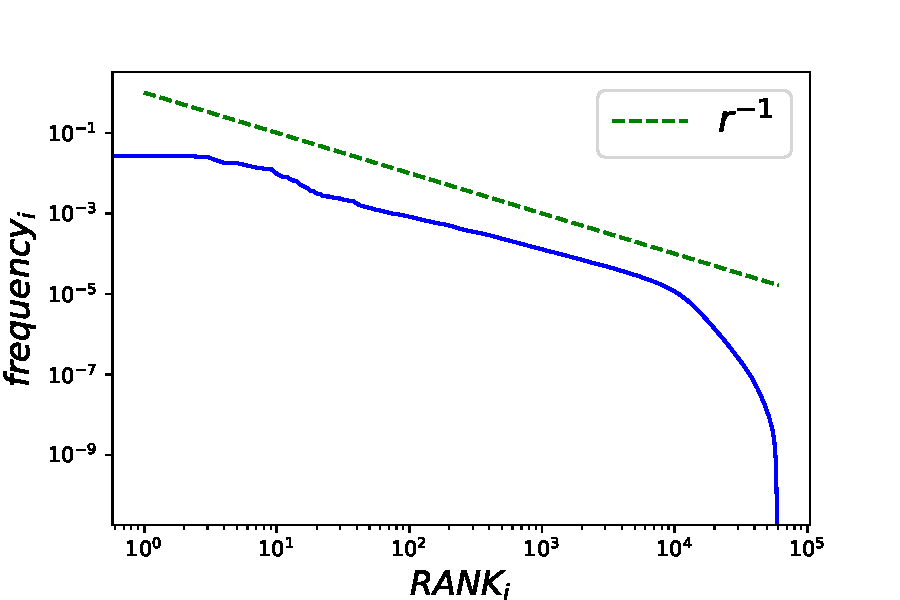
\includegraphics[width=0.95\linewidth]{pictures/structure/tcga/globalzipf_fpkmall.pdf}
    \end{minipage}
\hspace{3mm}
    \begin{minipage}{0.45\textwidth}
    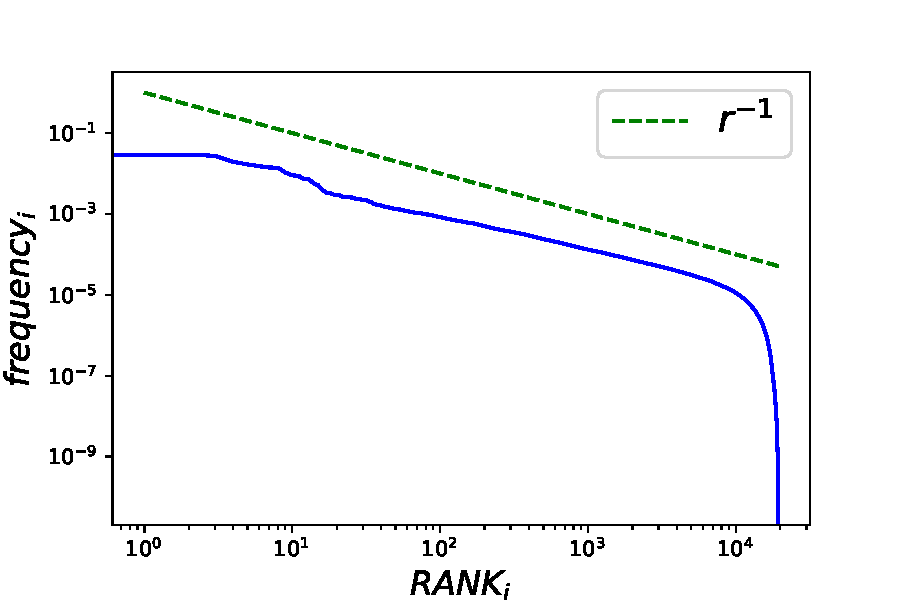
\includegraphics[width=0.95\linewidth]{pictures/structure/tcga/globalzipf_fpkm.pdf}
    \end{minipage}
    \caption{Zipf's law from FPKM normalised data. On the right considering only protein coding genes}
    \label{fig:structure/tcga/globalZipf}
\end{figure}
In figure~\ref{fig:structure/tcga/globalZipf} it is shown the frequency ranked plot. It is interesting that this kind of data distribute according a power law with exponent close to $1$, this same behaviour can be found in completely different systems such as linguistics' ones~\cite{altmann2016statistical}. Another interesting fact is that considering in the analysis also non-coding genes gives a double-scaled power law. This is due to the fact that non coding genes are also more specific and rare, so their frequencies are quite small compared to protein coding genes.

Changing normalisation and considering counts instead of FPKM, the result is quite similar. The power law is more flat, meaning that genes have more similar abundances in the whole dataset. 
\begin{figure}
    \centering
    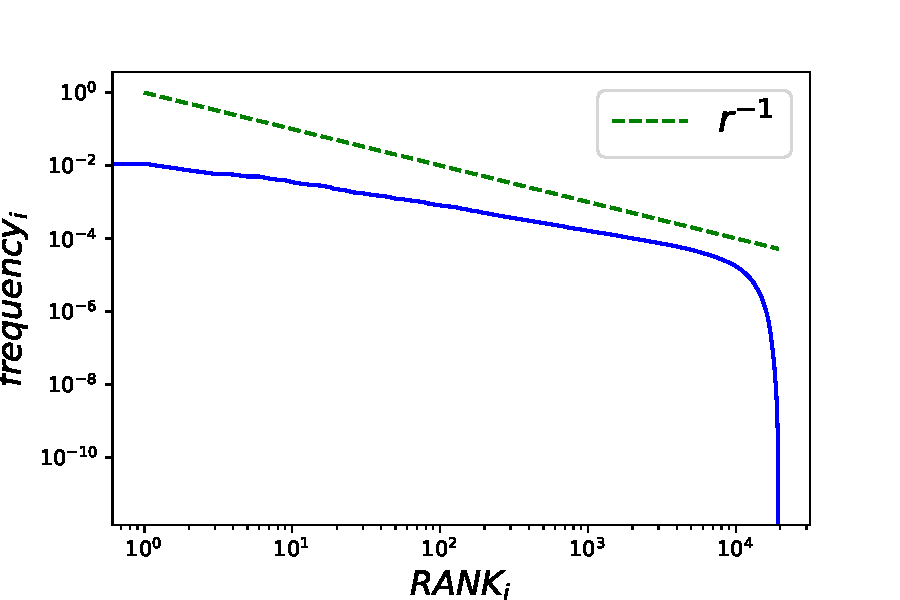
\includegraphics[width=0.8\linewidth]{pictures/structure/tcga/globalzipf_counts.pdf}
    \caption{Zipf's law of protein coding genes considering counts}
    \label{fig:structure/tcga/globalzipf_count}
\end{figure}

\subsection{GTEx}
A pretty similar analysis can be made on GTEx's~\cite{carithers2015novel} healthy samples. RNA sequencing raw counts data were download from file version \textit{2016-01-15 v7 RNASeQCv1.1.8}. All $\sim 11000$ samples available were considered at this time.

\begin{figure}[htb!]
    \centering
    \begin{minipage}{0.45\textwidth}
    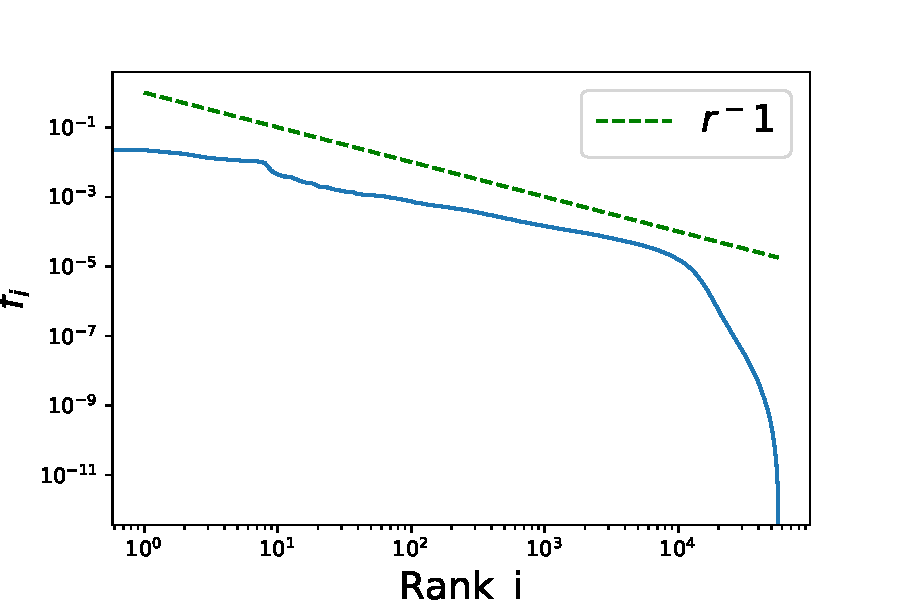
\includegraphics[width=0.95\linewidth]{pictures/structure/gtex/globalZipf.pdf}
    \end{minipage}
    \hspace{3mm}
    \begin{minipage}{0.45\textwidth}
    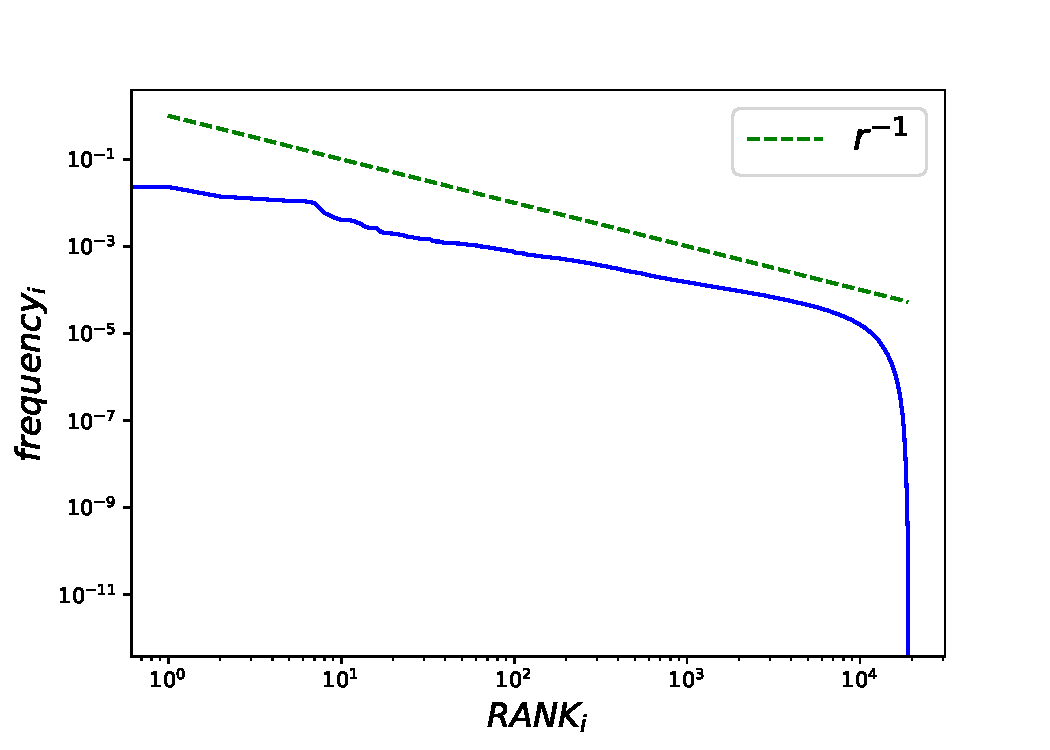
\includegraphics[width=0.95\linewidth]{pictures/structure/gtex/globalZipf_c.pdf}
    \end{minipage}
    \caption{Zipf's law from GTEx count data. On the left all genes considered, on the right only protein coding ones}
    \label{fig:my_label}
\end{figure}
Not surprisingly in the GTEx dataset it is retrieved the same behaviour at this time. The power law with exponent $\simeq 1$ is found and considering non coding genes lead to a knee in the power law.

Going further in the analysis it is possible make an histogram of occurrences defined by~\ref{eq:occurrence}, also known as $U$s.
\begin{figure}[htb!]
    \centering
    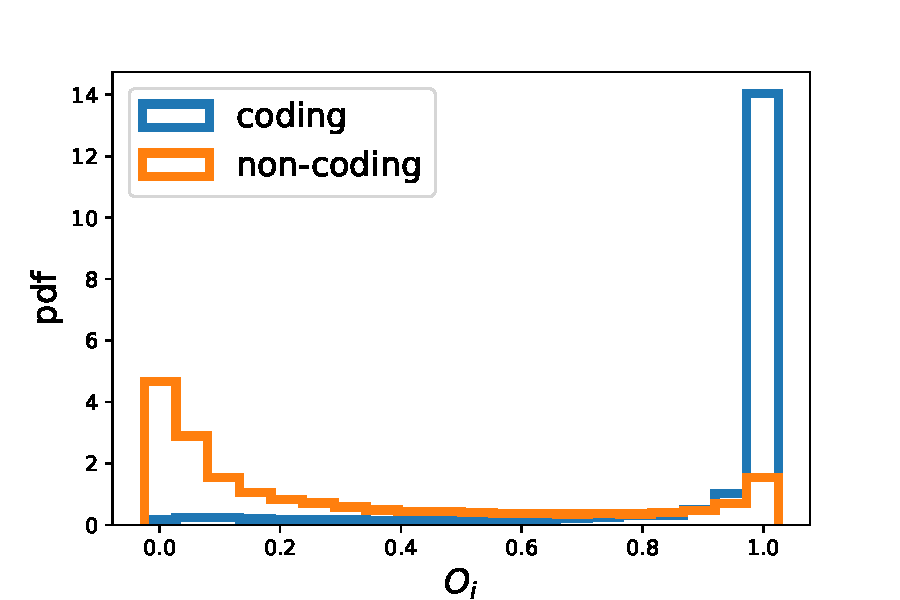
\includegraphics[width=0.9\linewidth]{pictures/structure/gtex/U_gtex_cnc.pdf}
    \caption{The histogram of the occurrences $O_i$}
    \label{fig:structure/gtex/U_cnc}
\end{figure}

Also in this kind of analysis it is possible to see the different behaviour of coding and not coding genes. The protein coding genes express almost in every sample, so their occurrence is near to $1$, non coding genes are more specific, so they are present only in a subset of the dataset and many of the have small occurrence.
\begin{figure}[htb!]
    \centering
    \begin{minipage}{0.45\textwidth}
    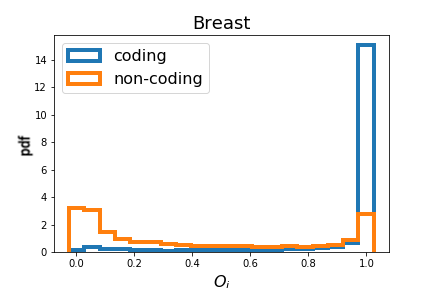
\includegraphics[width=0.95\linewidth]{pictures/structure/gtex/U_Breast.png}
    \end{minipage}
    \hspace{2mm}
    \begin{minipage}{0.45\textwidth}
    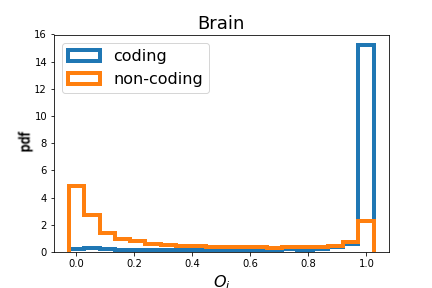
\includegraphics[width=0.95\linewidth]{pictures/structure/gtex/U_Brain.png}
    \end{minipage}
    \caption{Same behaviour is observed looking at one tissue a time.}
    \label{fig:structure/gtex/U_tissues}
\end{figure}
The same behaviour can be observed considering just all samples of a given tissue. In this case $O_i=0$ means that the genes has a non zero expression in just one of the samples of the tissue considered; in other words if a gene never express in a tissue it is not considered when constructing these tissue specific $U$ distributions.

From now on except were explicitly declared analysis will be made considering protein coding genes and counts with no normalisation.


%%null model
\section{Null model construction}\label{sec:nullmodel}
The kind of data considered in this work comes from RNA Sequencing experiments. These experiments use wet biology methods to extract information from samples. If one imagines it exists an unknown function that describes the gene expression across the samples considered, what experimental people do is to sample this function, picking up some genes.

In this section it is described a null model of sampling, this is useful to verify if the data distributions seen are just an effect of this experimental sample or if they carry some useful and interesting information.

As described in~\cite{Mazzolini2018}, a random matrix has to be created. This matrix is a collection of components and realizations exactly as~\ref{fig:componetstable}. The values of each component abundances in each realization $n_{i j}$ are randomly assigned with a probability determined by 
the global abundance in the whole dataset~\ref{eq:abundance}. Values of each column are extracted until the size~\ref{eq:size} is 
reached. Strictly speaking it is a multinomial process with probability
\begin{equation}
P\left( \{ n_i\} ;M\right) =\frac{M!}{\prod_{i=1}^{N} n_i}\prod_{i=1}^N f_i^{n_i}
\end{equation}
where $n_i$ is the number of times the component with frequency $f_i$ appears, being $f_i=\frac{a_i}{\sum_{c=1}^{N}a_{c}}$ as defined in~\ref{eq:fi}.

Figure~\ref{fig:structure/randomsampling} shows an example of this, $M$ components are picked up concerning their frequency in the dataset. The most abundant components, which are also the ones with the highest frequencies (frequency is nothing but the normalized abundance), have a greater probability to be picked up.
\begin{figure}[htb!]
    \centering
    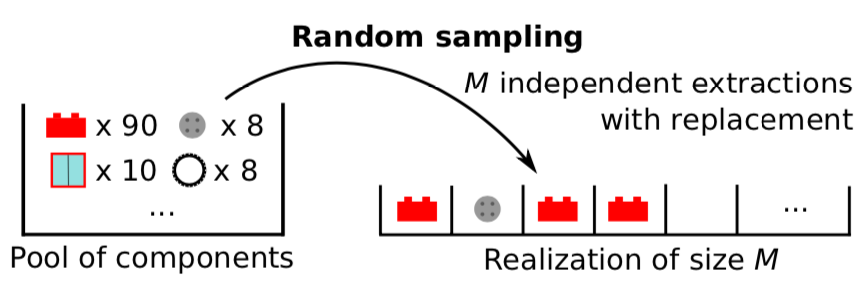
\includegraphics[width=0.8\linewidth]{pictures/structure/randomsampling.png}
    \caption{Random sampling of components to build a realization of size $M$.}
    \label{fig:structure/randomsampling}
\end{figure}

Using this construction on real counts data, by definition the Zipf's law sampled is identical to the data's one.
\begin{figure}[htb!]
\begin{minipage}{0.5\textwidth}
    \centering
    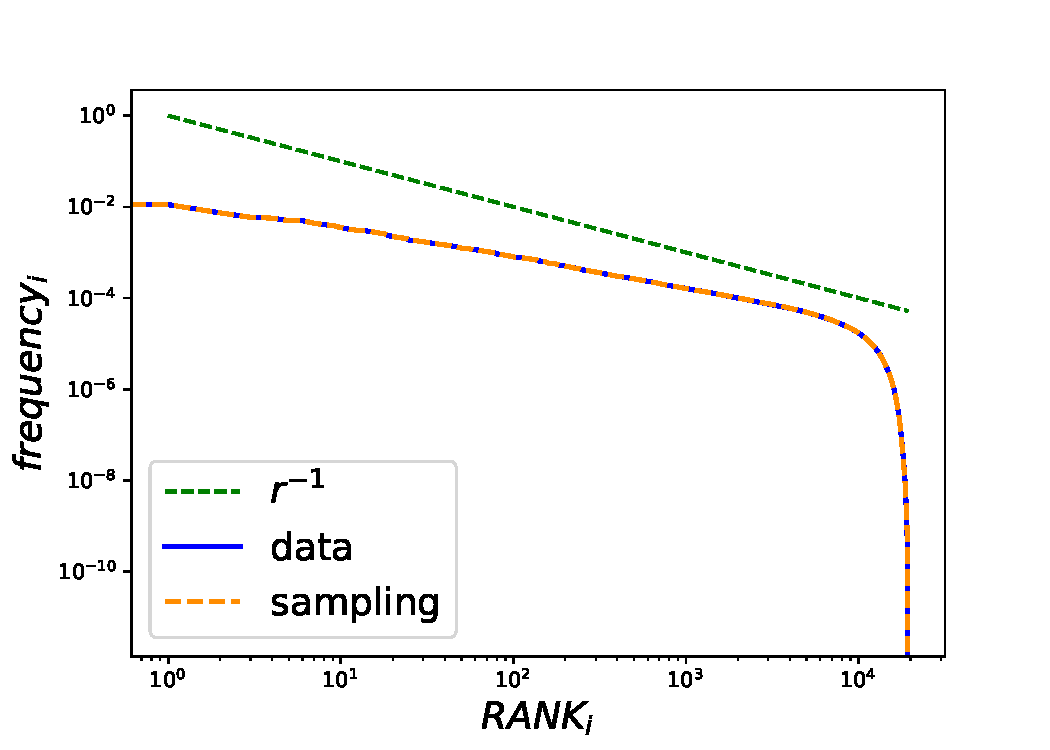
\includegraphics[width=0.95\linewidth]{pictures/structure/tcga/globalzipf_null.pdf}
\end{minipage}
\hspace{2mm}
\begin{minipage}{0.5\textwidth}
    \centering
    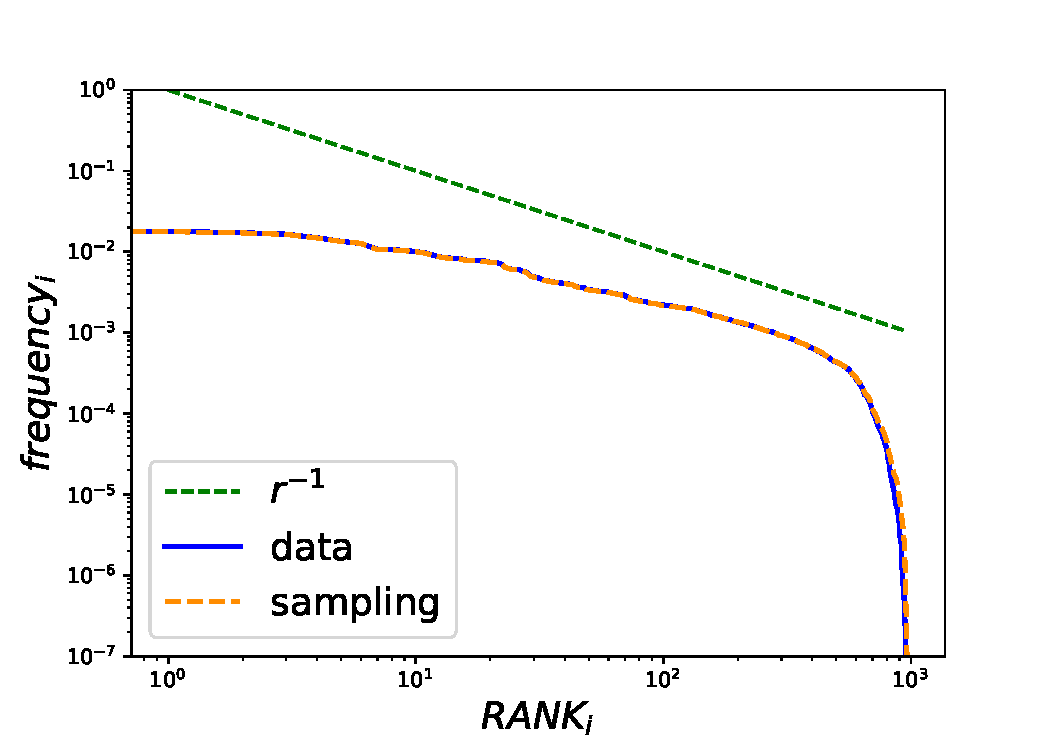
\includegraphics[width=0.95\linewidth]{pictures/structure/gtex/globalzipf_null.pdf}
\end{minipage}
\caption{Zipf's law sampled; TCGA(left) and GTEx (right). By definition original frequencies and sampled ones are identical.}
\label{fig:structure/globalzipf_null}
\end{figure}
By construction, the distribution of the sizes of the sampling and the data are also identical.
\begin{figure}[htb!]
\begin{minipage}{0.5\textwidth}
    \centering
    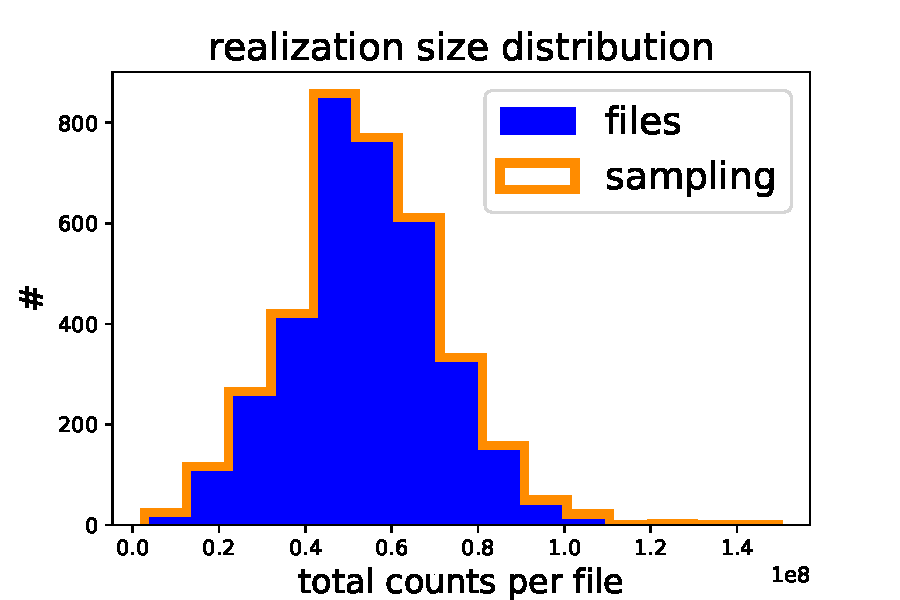
\includegraphics[width=0.95\linewidth]{pictures/structure/tcga/sizeDistr_null.pdf}
\end{minipage}
\hspace{2mm}
\begin{minipage}{0.5\textwidth}
    \centering
    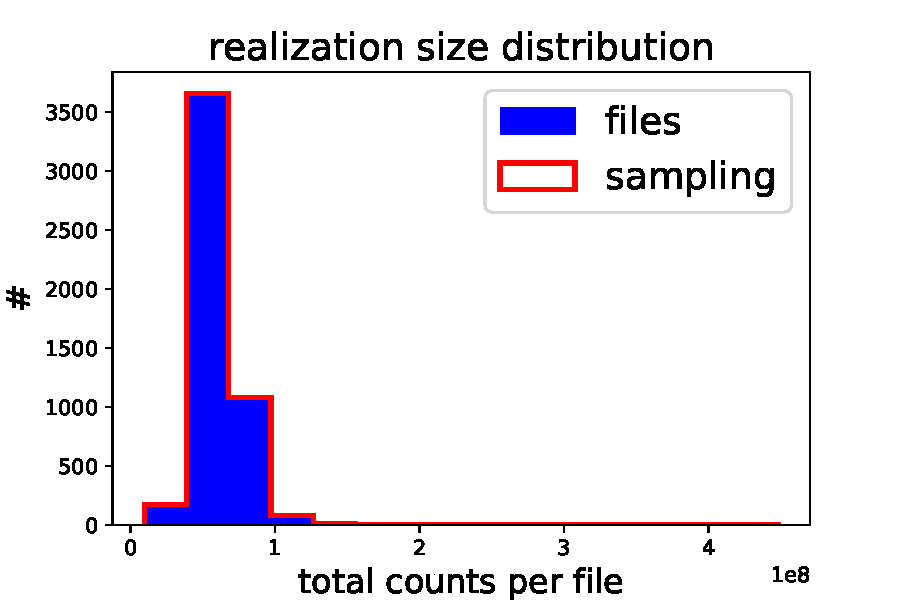
\includegraphics[width=0.95\linewidth]{pictures/structure/gtex/sizeDistr_null.pdf}
    \end{minipage}
\caption{Distribution of sizes $M$; TCGA(left) and GTEx (right). By definition sampling and original sizes are identical.}
    \label{fig:structure/sizeDistr_null}
\end{figure}

Looking at the $U$s in figure~\ref{fig:structure/globalU_null}, it is evident that data behave differently from sampling. This is a signal that the null model is not enough to explain the data matrices. In particular, it is evident that the null model generates the matrices in a manner such that more components have high occurrence comparing to the original data. This can be easily explained, in fact in the real world some genes are highly expressed but only in a subset of the whole dataset; these genes are specific for certain type of samples. The null model gets the information that such genes are highly expressed (they have a high abundance) and so samples these quite often (components with high abundance have a greater chance to be picked up by the null model sampling). This set of genes with $O_i=1$ is called \textbf{core}, in figure~\ref{fig:structure/globalU_null} it is evident the difference between the real one and the sampled one.
\begin{figure}[htb!]
\begin{minipage}{0.5\textwidth}
    \centering
    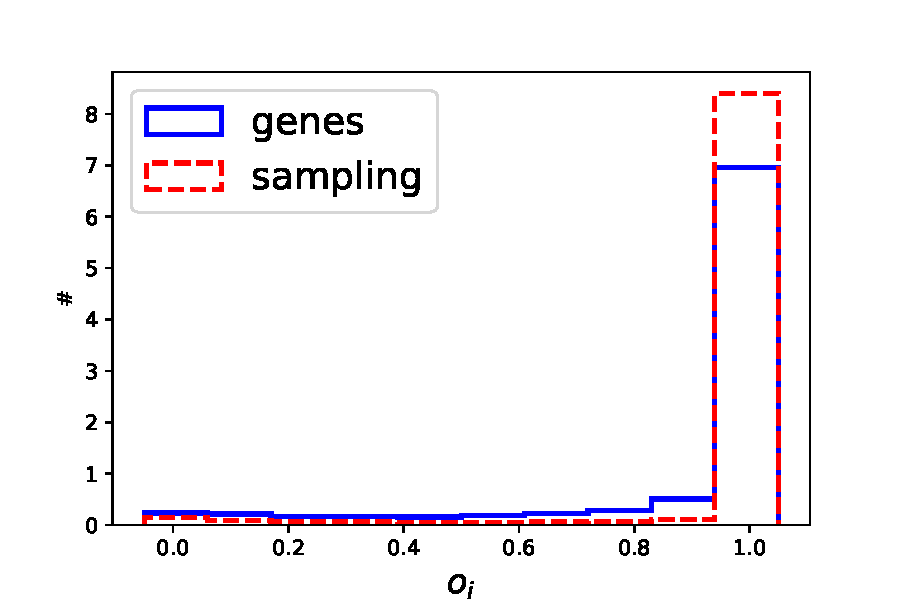
\includegraphics[width=0.95\linewidth]{pictures/structure/tcga/globalU_null.pdf}
\end{minipage}
\hspace{2mm}
\begin{minipage}{0.5\textwidth}
    \centering
    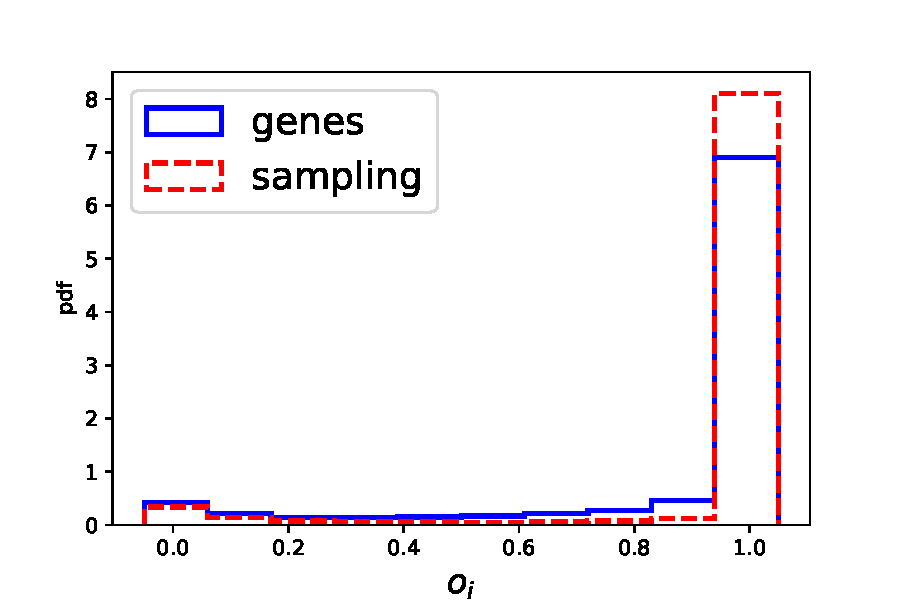
\includegraphics[width=0.95\linewidth]{pictures/structure/gtex/globalU_null.pdf}
    \end{minipage}
\caption{Occurrence distributions; TCGA(left) and GTEx (right). Sampling is reported for comparison.}
\label{fig:structure/globalU_null}
\end{figure}

Plotting on the abscissa the size of samples and on the ordinate the number of genes expressed one point per sample, it is possible to obtain the so-called Heaps's law~\cite{Heaps:1978:IRC:539986}. In figure~\ref{fig:structure/heaps_null} the Heaps' law is presented compared to the one obtained by sampling. Again the curves differ and the null model is not enough to explain the trend. Note that each data point shares the abscissa with a sampling one (figures~\ref{fig:structure/sizeDistr_null} are nothing but the histograms of the abscissas of~\ref{fig:structure/heaps_null}). Moreover, it is interesting that the ordinate does not start from zero, this happens because there are a lot of genes that express everywhere, the core. It happens that the sampling curve is translated above the data's one. This means that to build a sample of size $M$ just by sampling it is necessary to use a greater number of different genes than the number of different genes actually expressed in nature. In other words in the real world only the genes that are really useful in a sample are expressed, and this is not describable just by sampling. This fact is coherent with the fact that the $U$s differ.
\begin{figure}[htb!]
\begin{minipage}{0.5\textwidth}
    \centering
    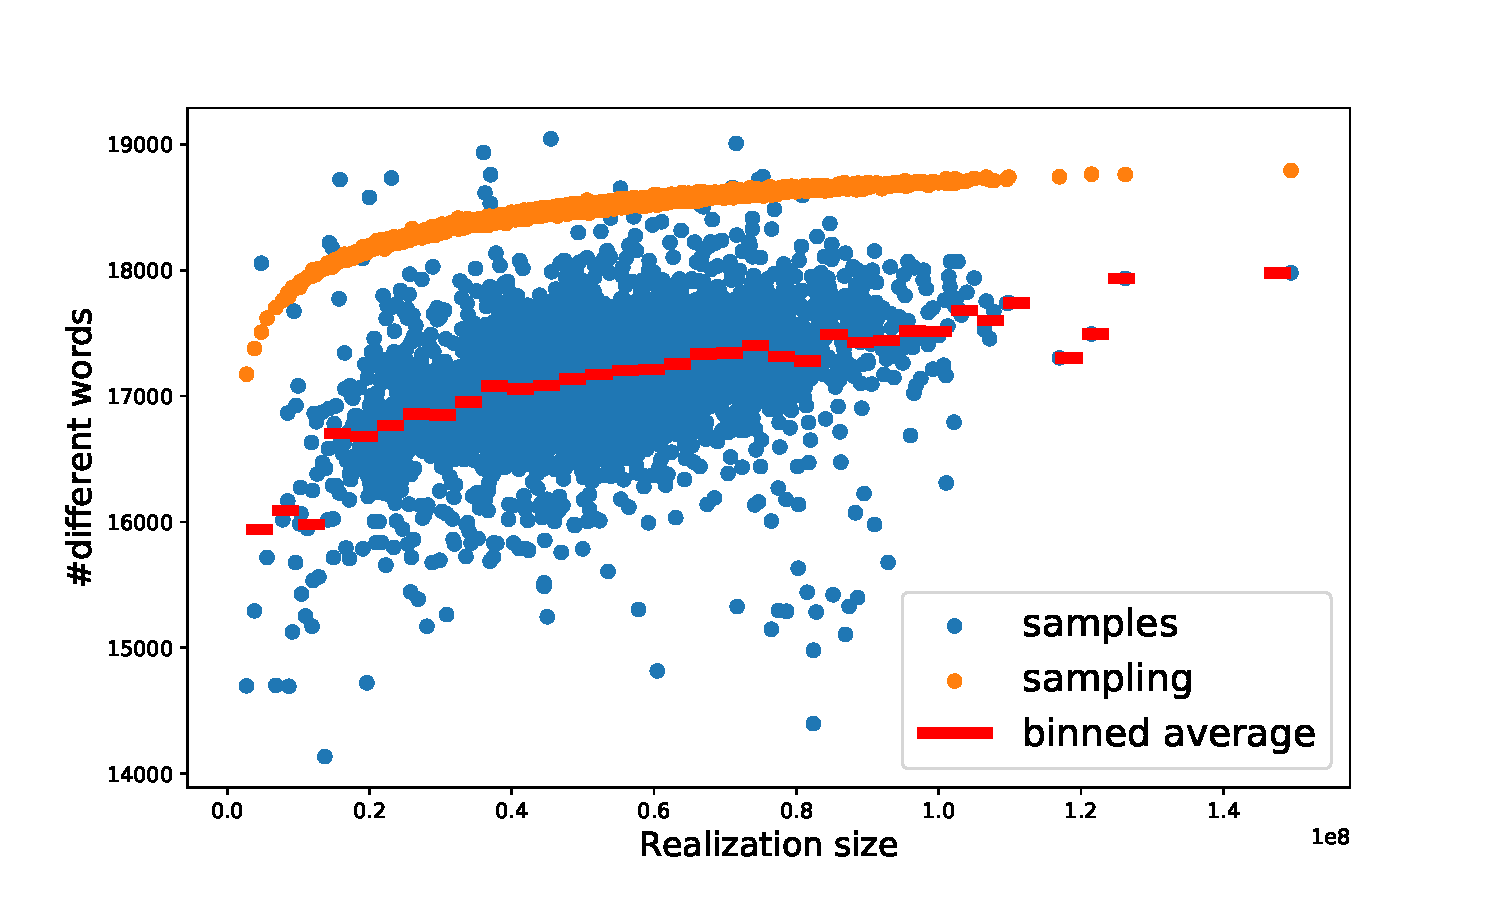
\includegraphics[width=0.95\linewidth]{pictures/structure/tcga/heaps_null.pdf}
    \end{minipage}
\hspace{2mm}
\begin{minipage}{0.5\textwidth}
    \centering
    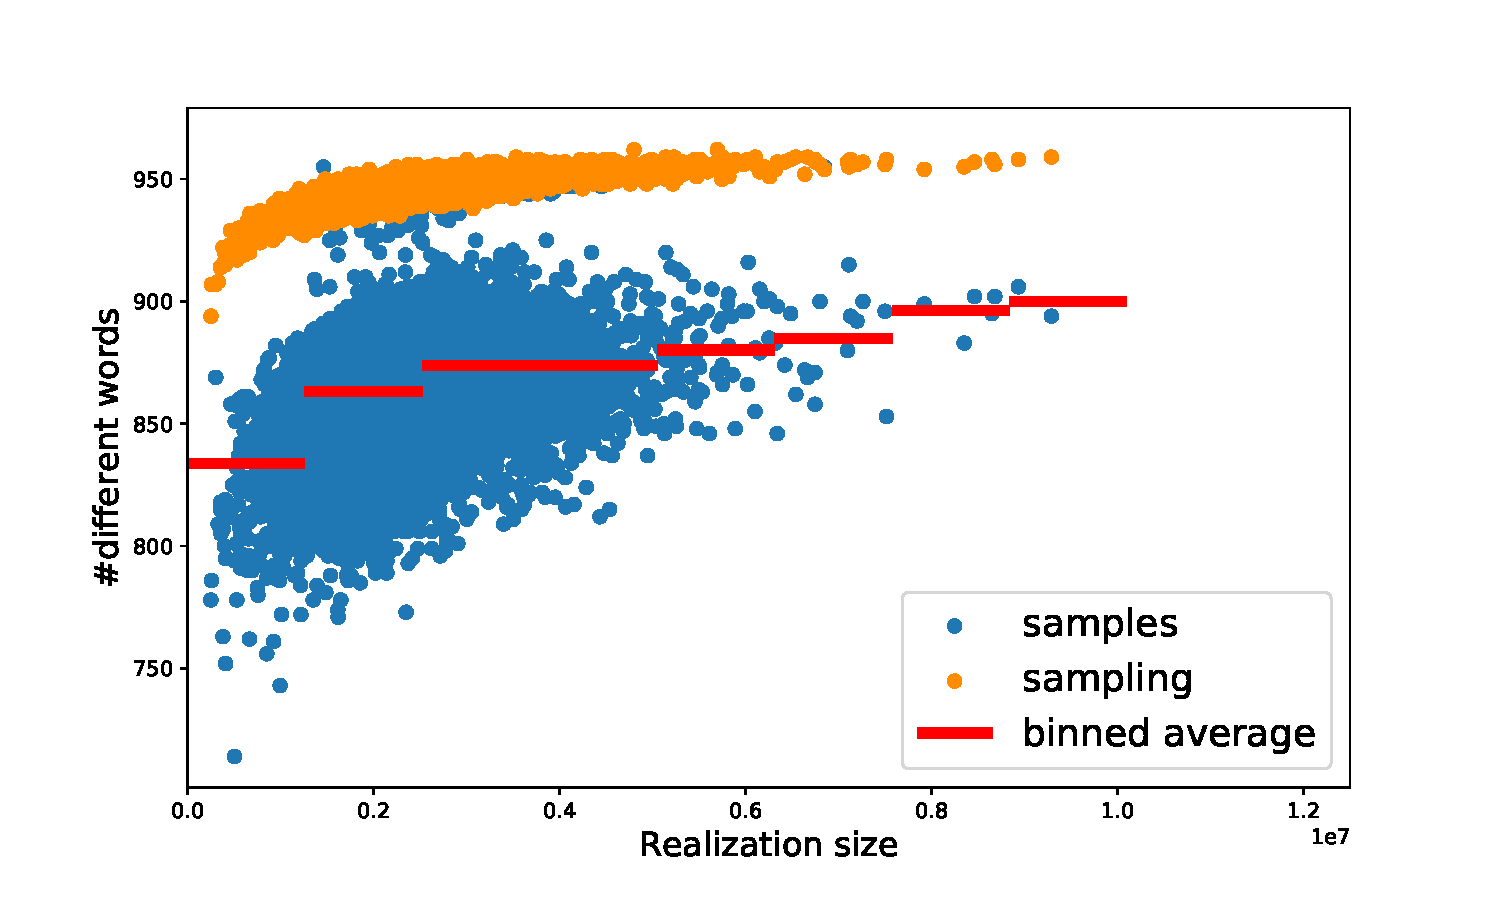
\includegraphics[width=0.95\linewidth]{pictures/structure/gtex/heaps_null.pdf}
    \end{minipage}
\caption{Heaps' law; TCGA(left) and GTEx (right). Sampling is reported for comparison.}
\label{fig:structure/heaps_null}
\end{figure}
Another way to see this is by looking at the histograms of the number of different genes expressed, actually the distribution of the~\ref{fig:structure/heaps_null} y-axis. Figure~\ref{fig:structure/diffwordsDistr_null} shows that these distributions are completely different if one looks at the data and the samples.
\begin{figure}[htb!]
\begin{minipage}{0.5\textwidth}
    \centering
    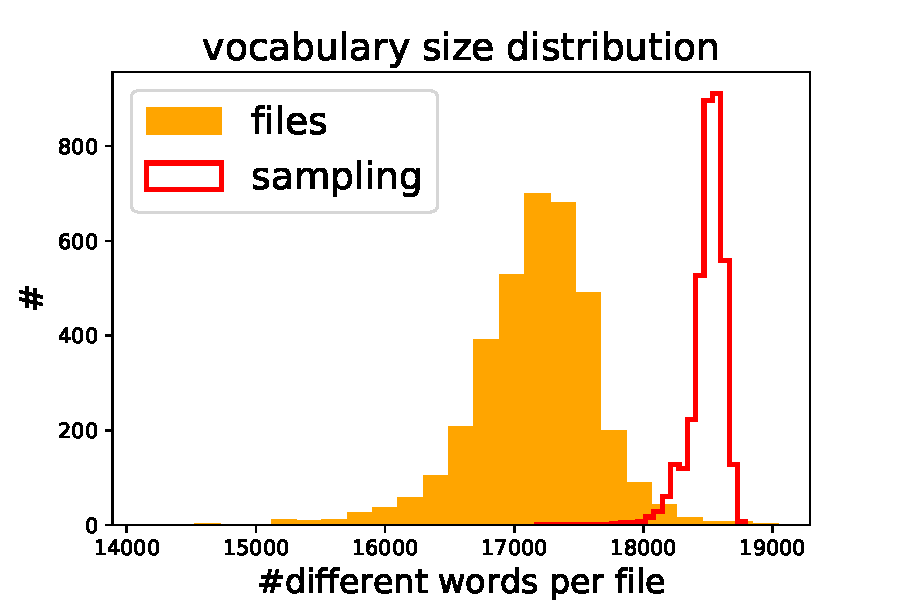
\includegraphics[width=0.95\linewidth]{pictures/structure/tcga/diffwordsDistr_null.pdf}
    \end{minipage}
\hspace{2mm}
\begin{minipage}{0.5\textwidth}
    \centering
    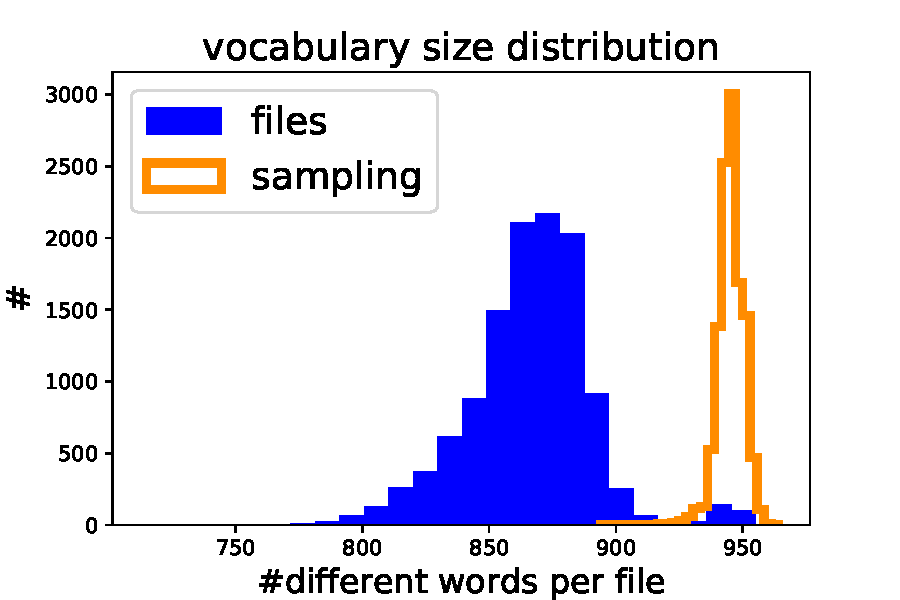
\includegraphics[width=0.95\linewidth]{pictures/structure/gtex/diffwordsDistr_null.pdf}
    \end{minipage}
\caption{Number of genes expressed in a sample; TCGA(left) and GTEx (right). The difference between the original data and sampling is evident.}
\label{fig:structure/diffwordsDistr_null}
\end{figure}

%%tissue differentation
%%tissue separation
\section{Statistical laws differentiate by tissue}
Observing the GTEx dataset of healthy samples it is possible to study how it is possible to see the tissue differentiation and how to study tissues' differences,~\cite{mele2014} suggests some approaches.

First of all, it could be interesting to study which is the fraction of transcriptome that can be explained by a certain number of genes.
To do this it is necessary to get all the samples of a given tissue. Then one estimates the average expression per each component (gene). At this point, one has the average abundance of each gene in a tissue, dividing by the sum of all the components it is possible to obtain the fraction of the total counts in the tissue due to each gene. Sorting from greater to smaller and integrating (cumulative summing) one have the fraction of transcript due to $1, 2, 3\dots$ genes. This is reported in figure~\ref{fig:structure/gtex/fraction_of_trascriptome}. This analysis is done using TPM to avoid biases due to gene lengths or to samples sizes.
\begin{figure}[htb!]
  \centering
  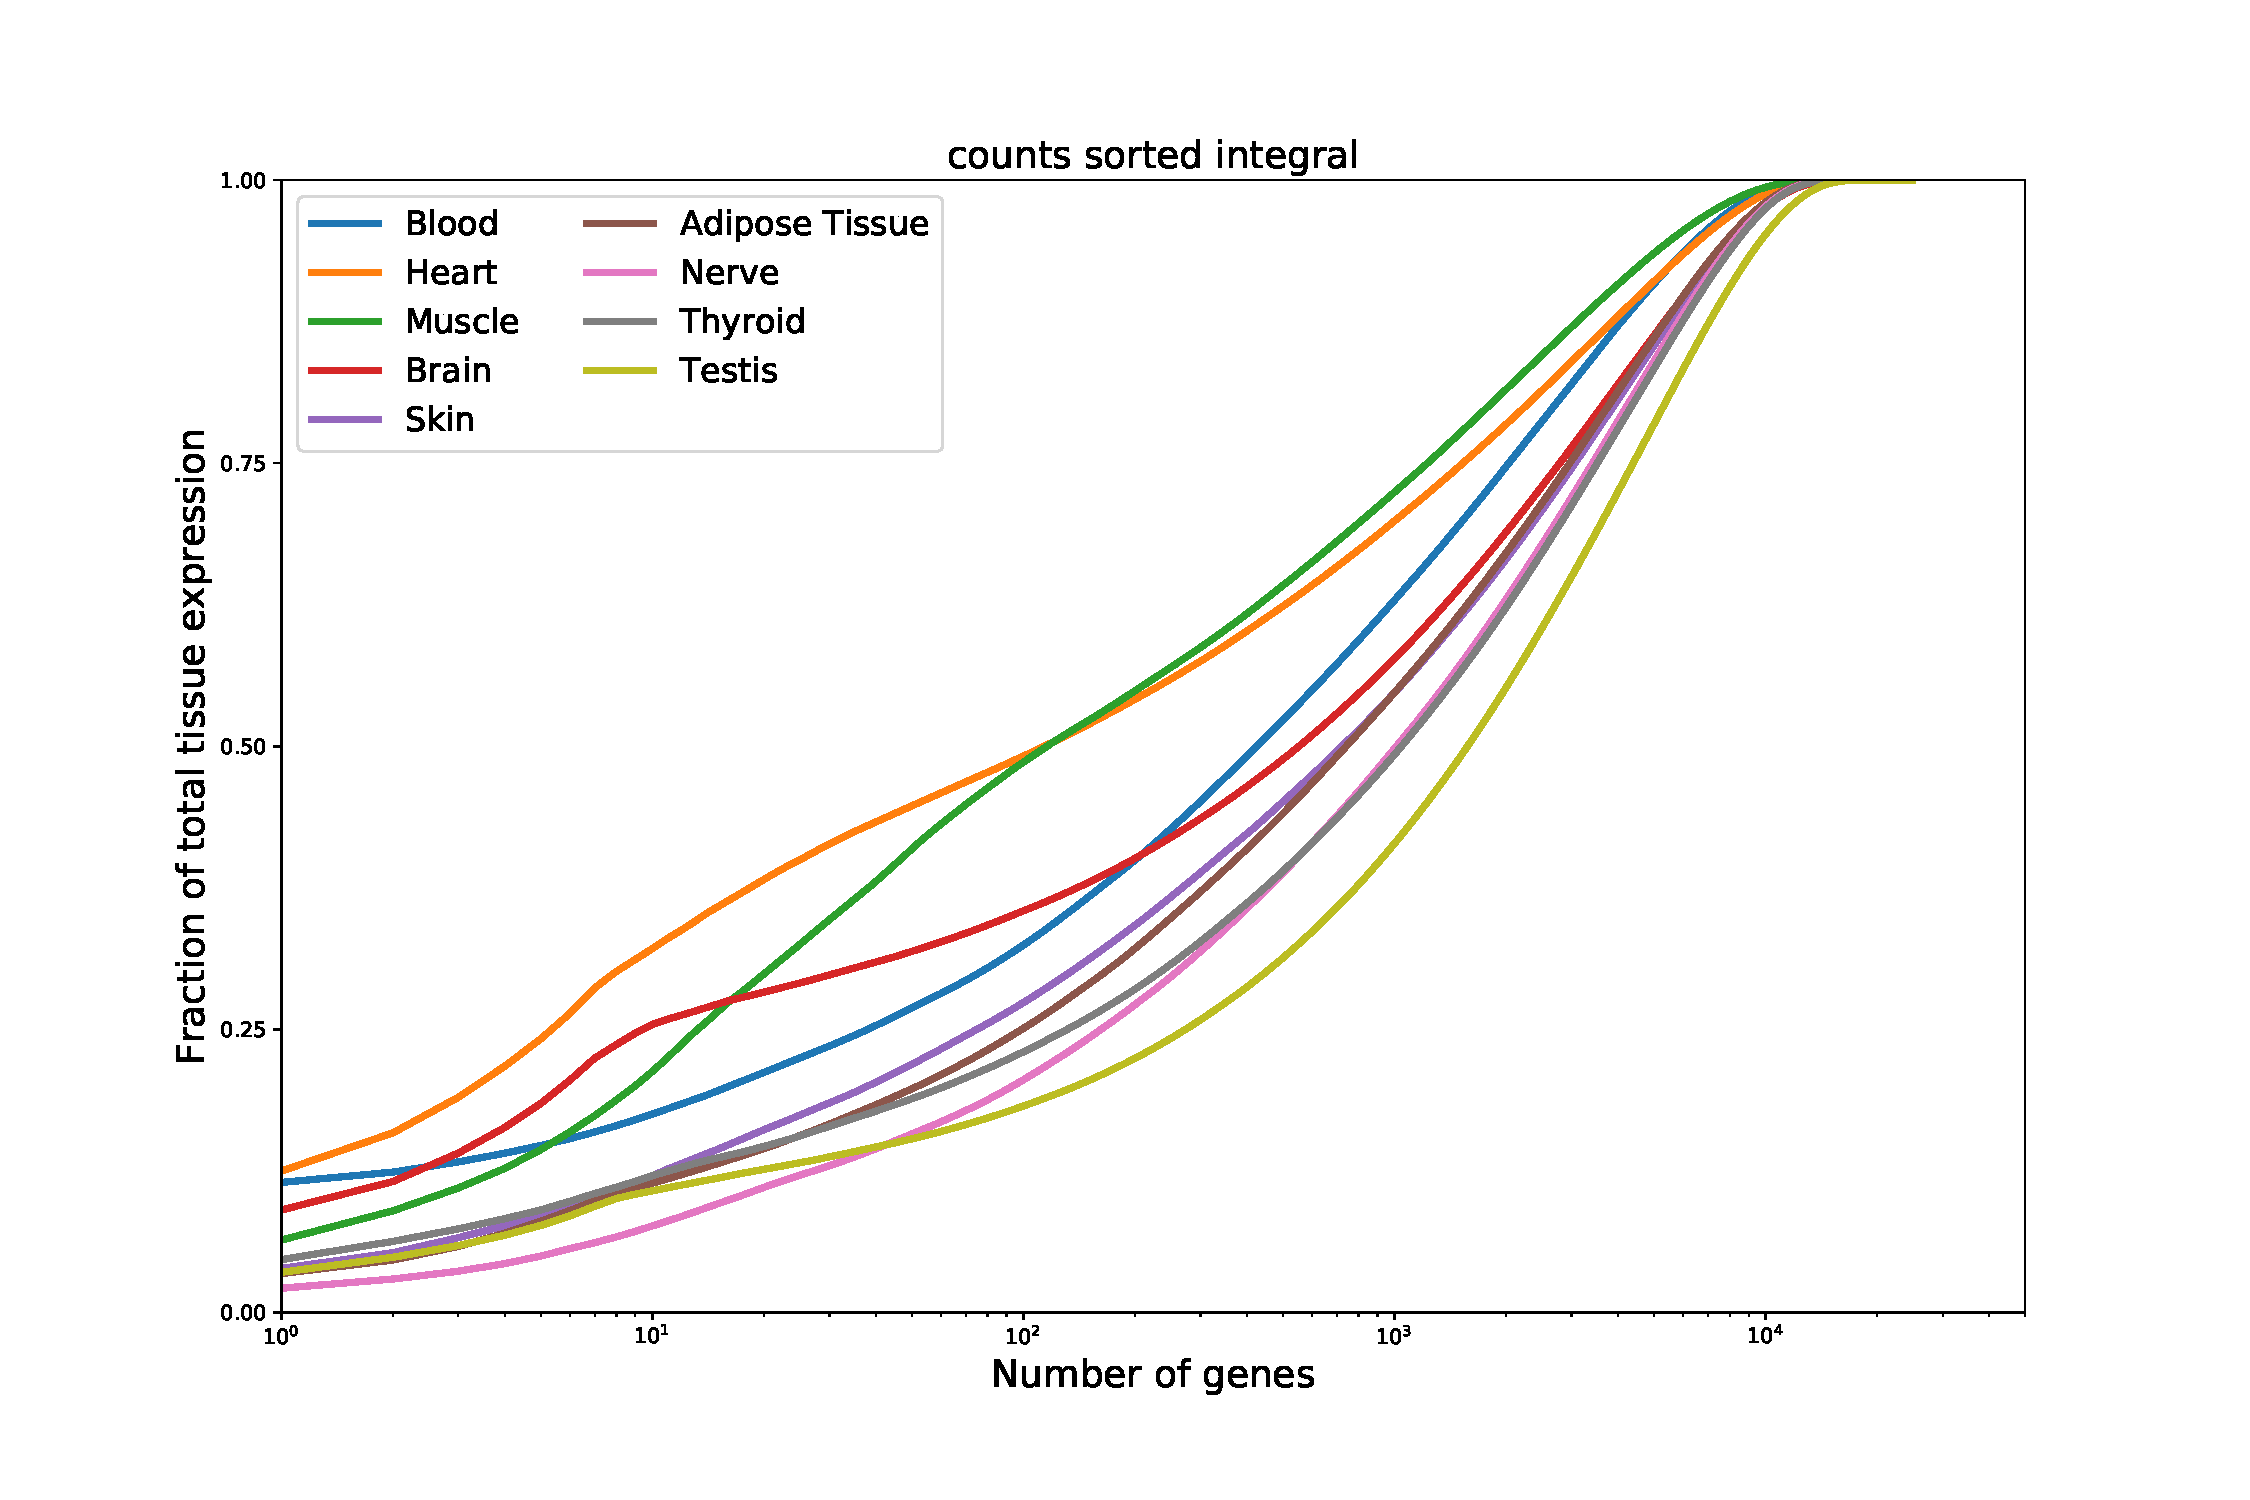
\includegraphics[width=0.7\linewidth]{pictures/structure/gtex/fraction_of_trascriptome.pdf}
  \caption{The integral of the sorted abundances for each tissue.}
  \label{fig:structure/gtex/fraction_of_trascriptome}
\end{figure}
Here, when a curve is steep it means that a few genes' expression represents a great fraction of the total size of the transcriptome. If a curve is smooth it means that many genes are necessary to describe the whole transcriptome for that particular tissue. This analysis shows that different tissues have a different complexity in terms of the number of genes necessary to build the transcriptome (in average). In figure~\ref{fig:structure/gtex/fraction_of_trascriptome_Brain} the same analysis is done for the sub-tissues of Brain, also this sub-type present a great separation.
\begin{figure}[htb!]
  \centering
  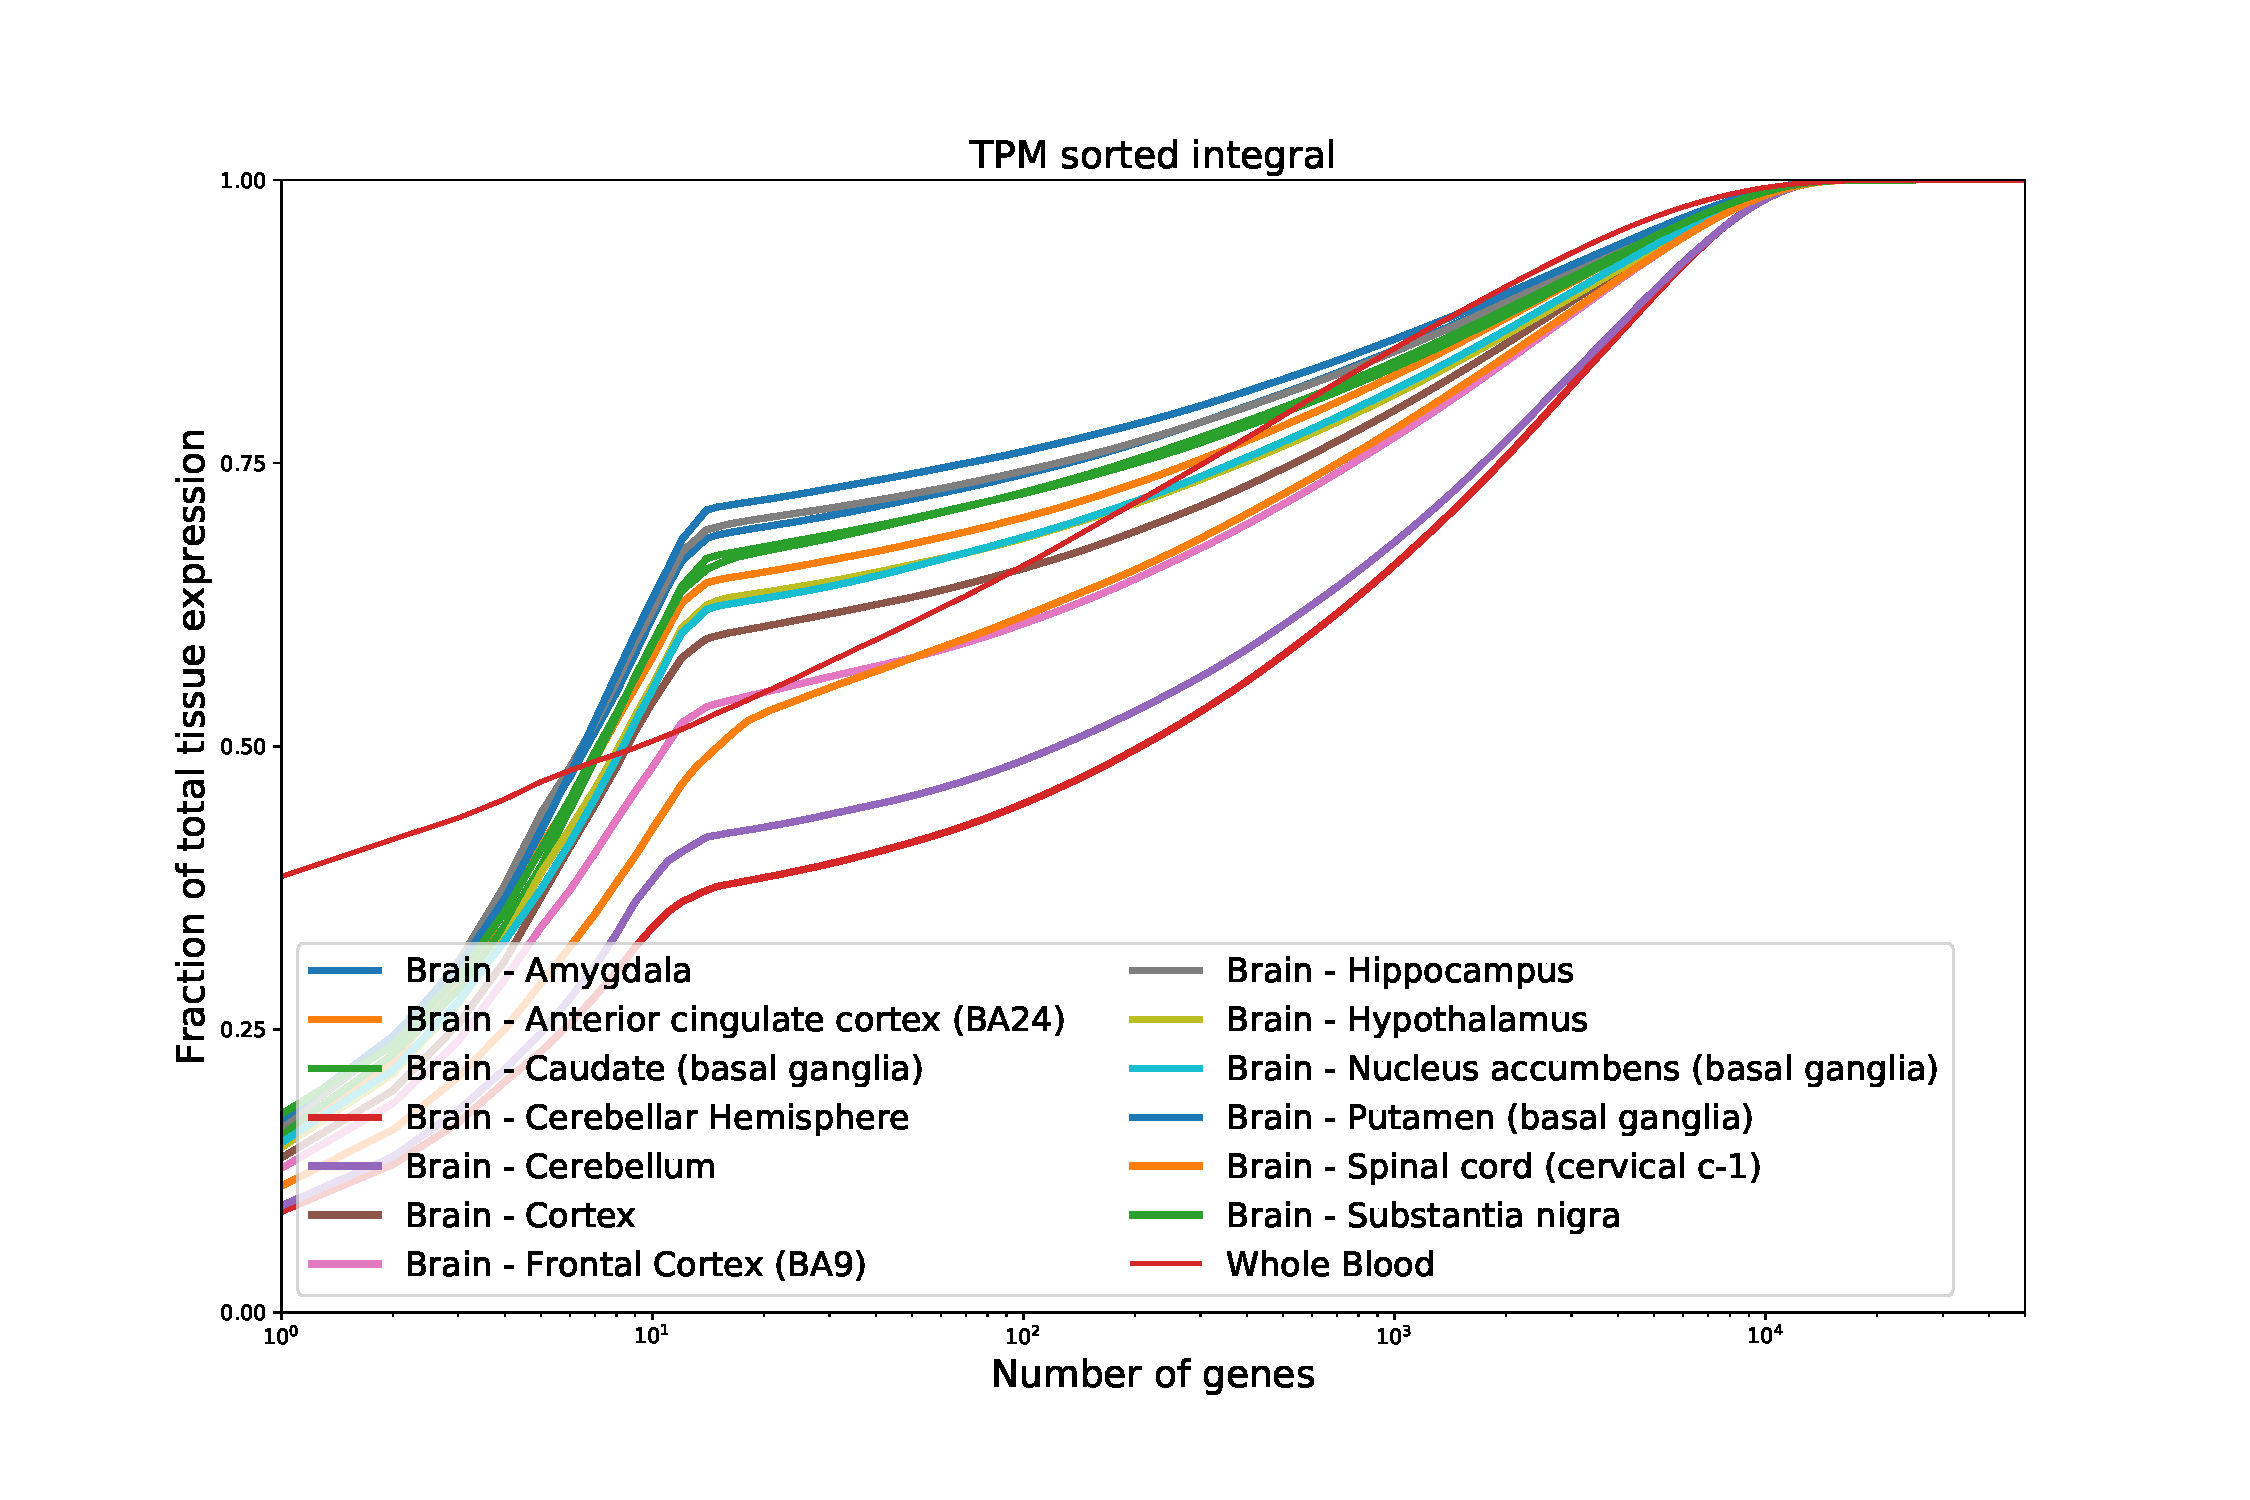
\includegraphics[width=0.65\linewidth]{pictures/structure/gtex/fraction_of_trascriptome_Brain.pdf}
  \caption{The integral of the sorted abundances for sub-types of Brain. This is done using TPM to avoid biases due to gene lengths. Blood is plotted for reference.}
  \label{fig:structure/gtex/fraction_of_trascriptome_Brain}
\end{figure}

Another way to interpret this analysis is thinking~\ref{fig:structure/gtex/fraction_of_trascriptome} as the integral of the Zipf's law. So it could be interesting to examine the Zipf one tissue a time. In figure~\ref{fig:structure/gtex/zipf_tissue} are reported the Zipf's law for some tissues with an extremal behaviour.
\begin{figure}[htb!]
  \centering
  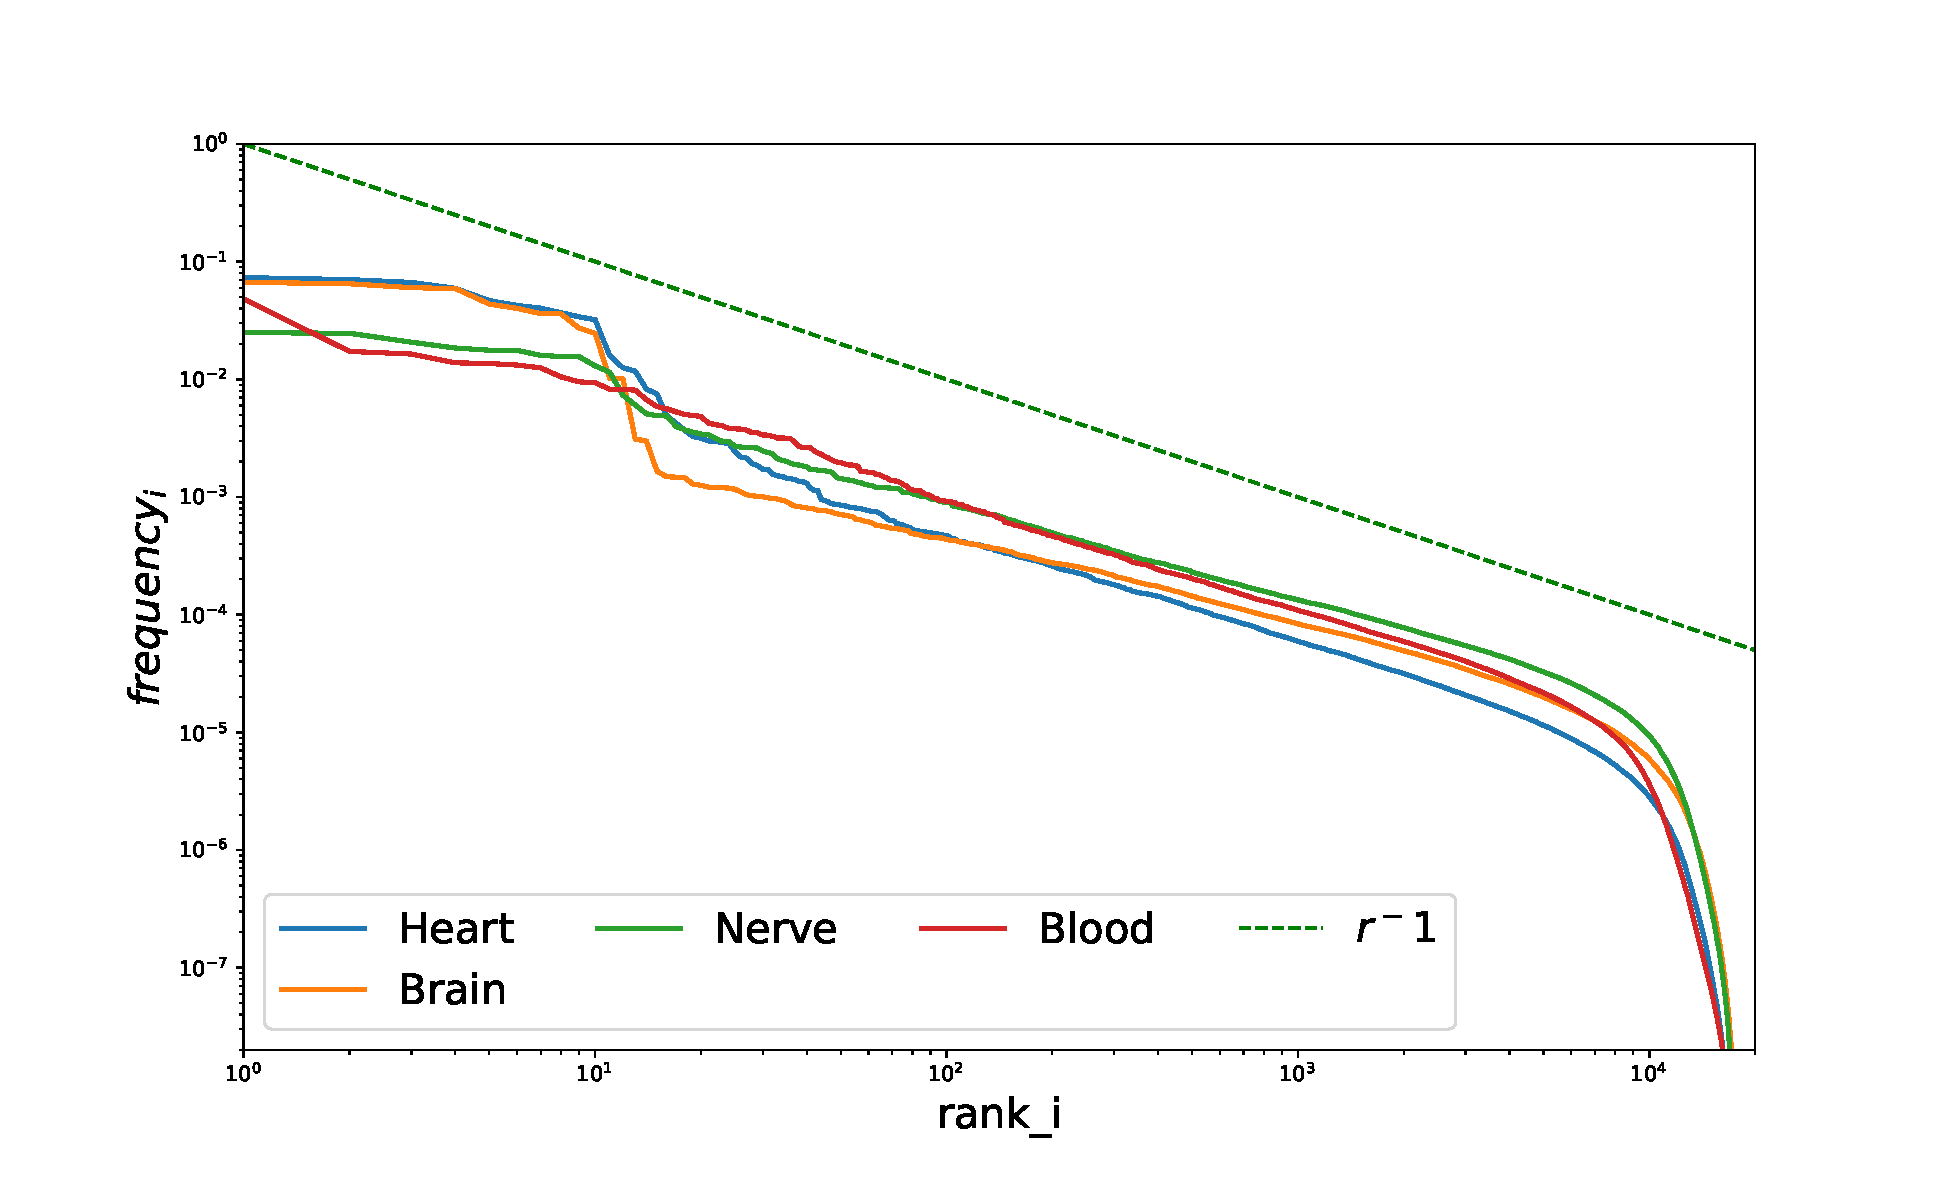
\includegraphics[width=0.45\linewidth]{pictures/structure/gtex/zipf_tissue.pdf}
  \caption{The integral of the sorted abundances for each tissue.}
  \label{fig:structure/gtex/zipf_tissue}
\end{figure}
From this point of view, each tissue has its particular slope. The steeper the Zipf the simplest is the tissue: the transcript can be described with few genes.

Coming back to the transcriptome analysis. In figure~\ref{fig:structure/gtex/fraction_of_trascriptome} the point where the curve reaches $1$ corresponds to the total number of genes expressed, the remaining ones have a $0$ expression and do not contribute to the transcript. This can be visualized again with the Heaps' law: the number of genes expressed seen in the Heaps' law plot is the number of genes necessary to explain the whole transcriptome. In figure~\ref{fig:structure/gtex/heaps_tissue}, it is evident that there is some kind of tissue differentiation even when looking at the Heaps' law. In other words, two samples with the same size but of different tissues have a different number of genes expressed.
\begin{figure}[htb!]
  \centering
  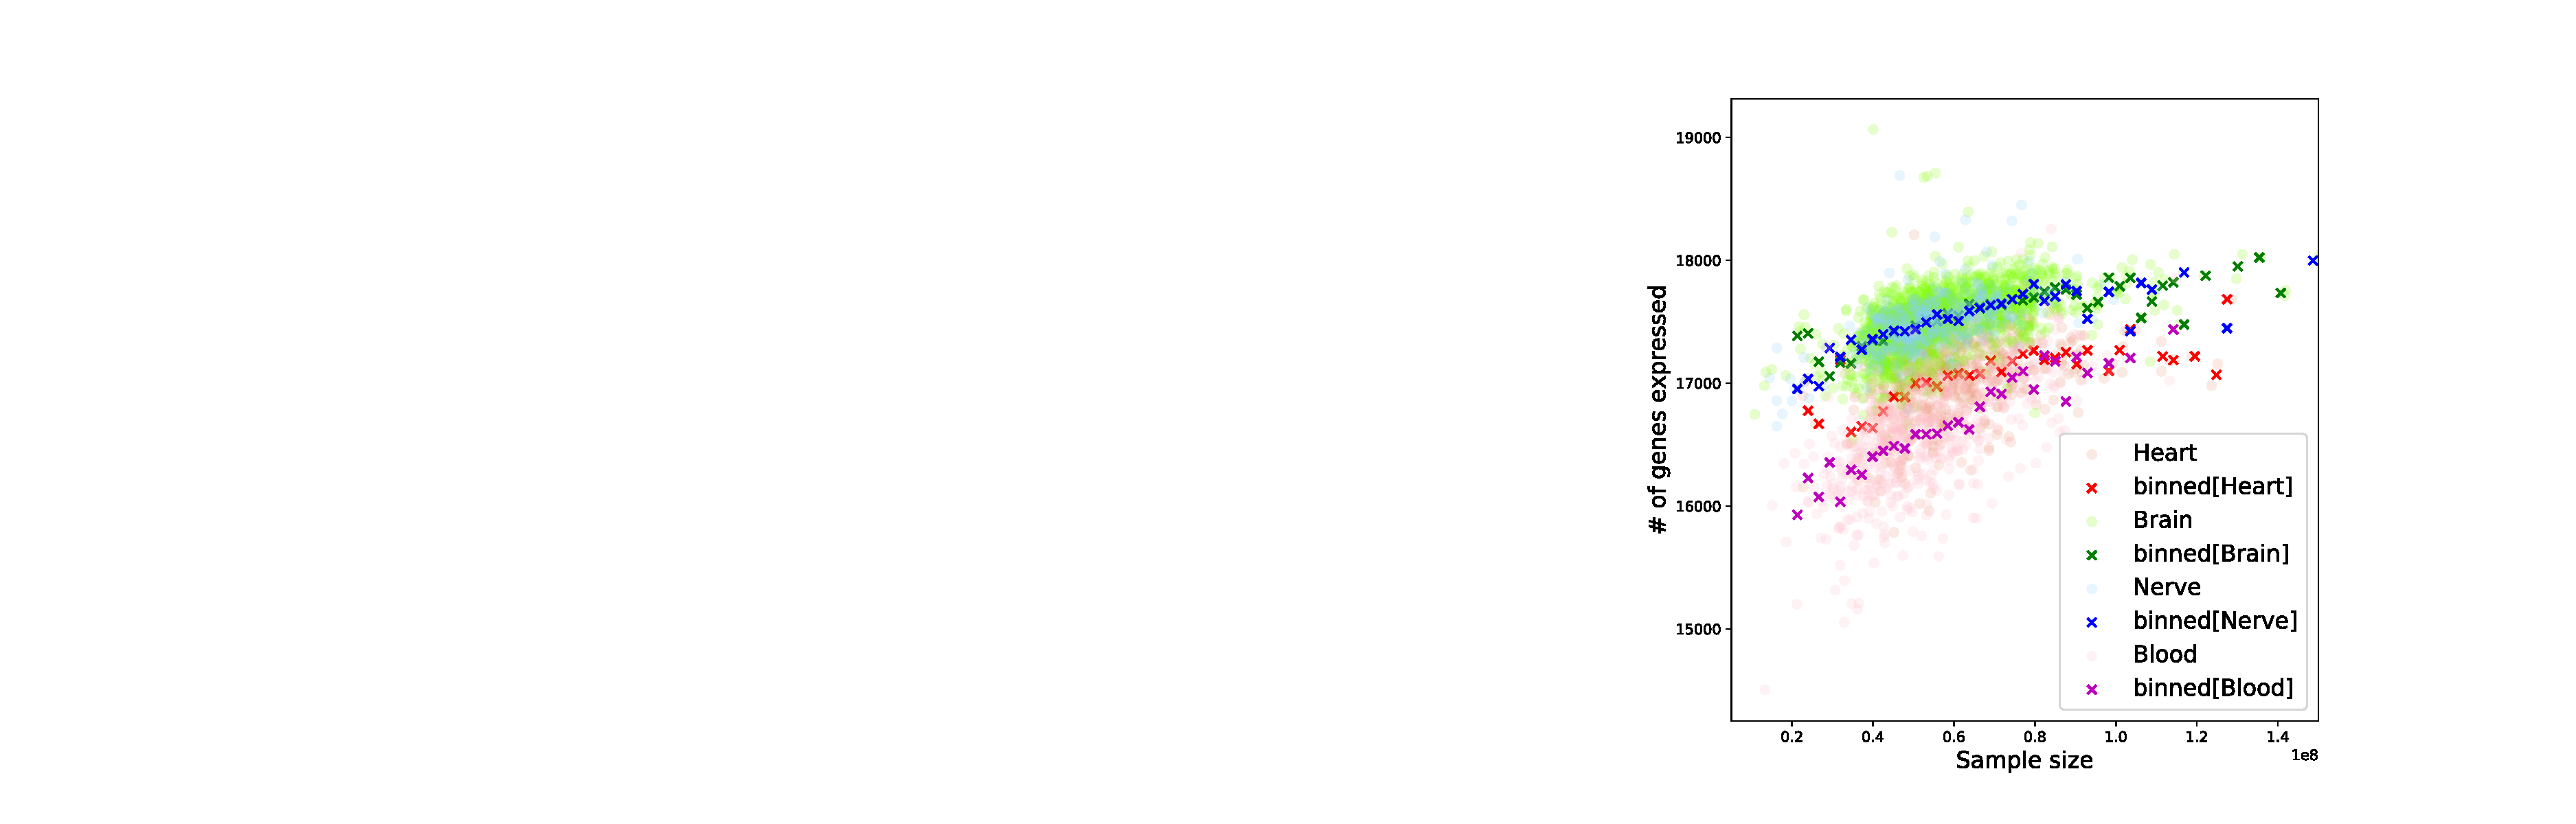
\includegraphics[width=0.5\linewidth]{pictures/structure/gtex/heaps_tissue.pdf}
  \caption{The integral of the sorted abundances for each tissue. This plot was done using counts, using TPM it is not possible because the size on the x-axis is a would be a constant.}
  \label{fig:structure/gtex/heaps_tissue}
\end{figure}
The same analysis can be made by looking at the disease type of cancer samples. In this case, there is no evident differentiation as shown in figure~\ref{fig:structure/tcga/fraction_of_trascriptome_disease}. The only diseases that behave differently are \textit{Parangliomas}, but these are associated only to Brain, so the differentiation seen is just a Brain separation. This means that separate diseases would be tricky and much more difficult than just separate tissues.
\begin{figure}[htb!]
  \centering
  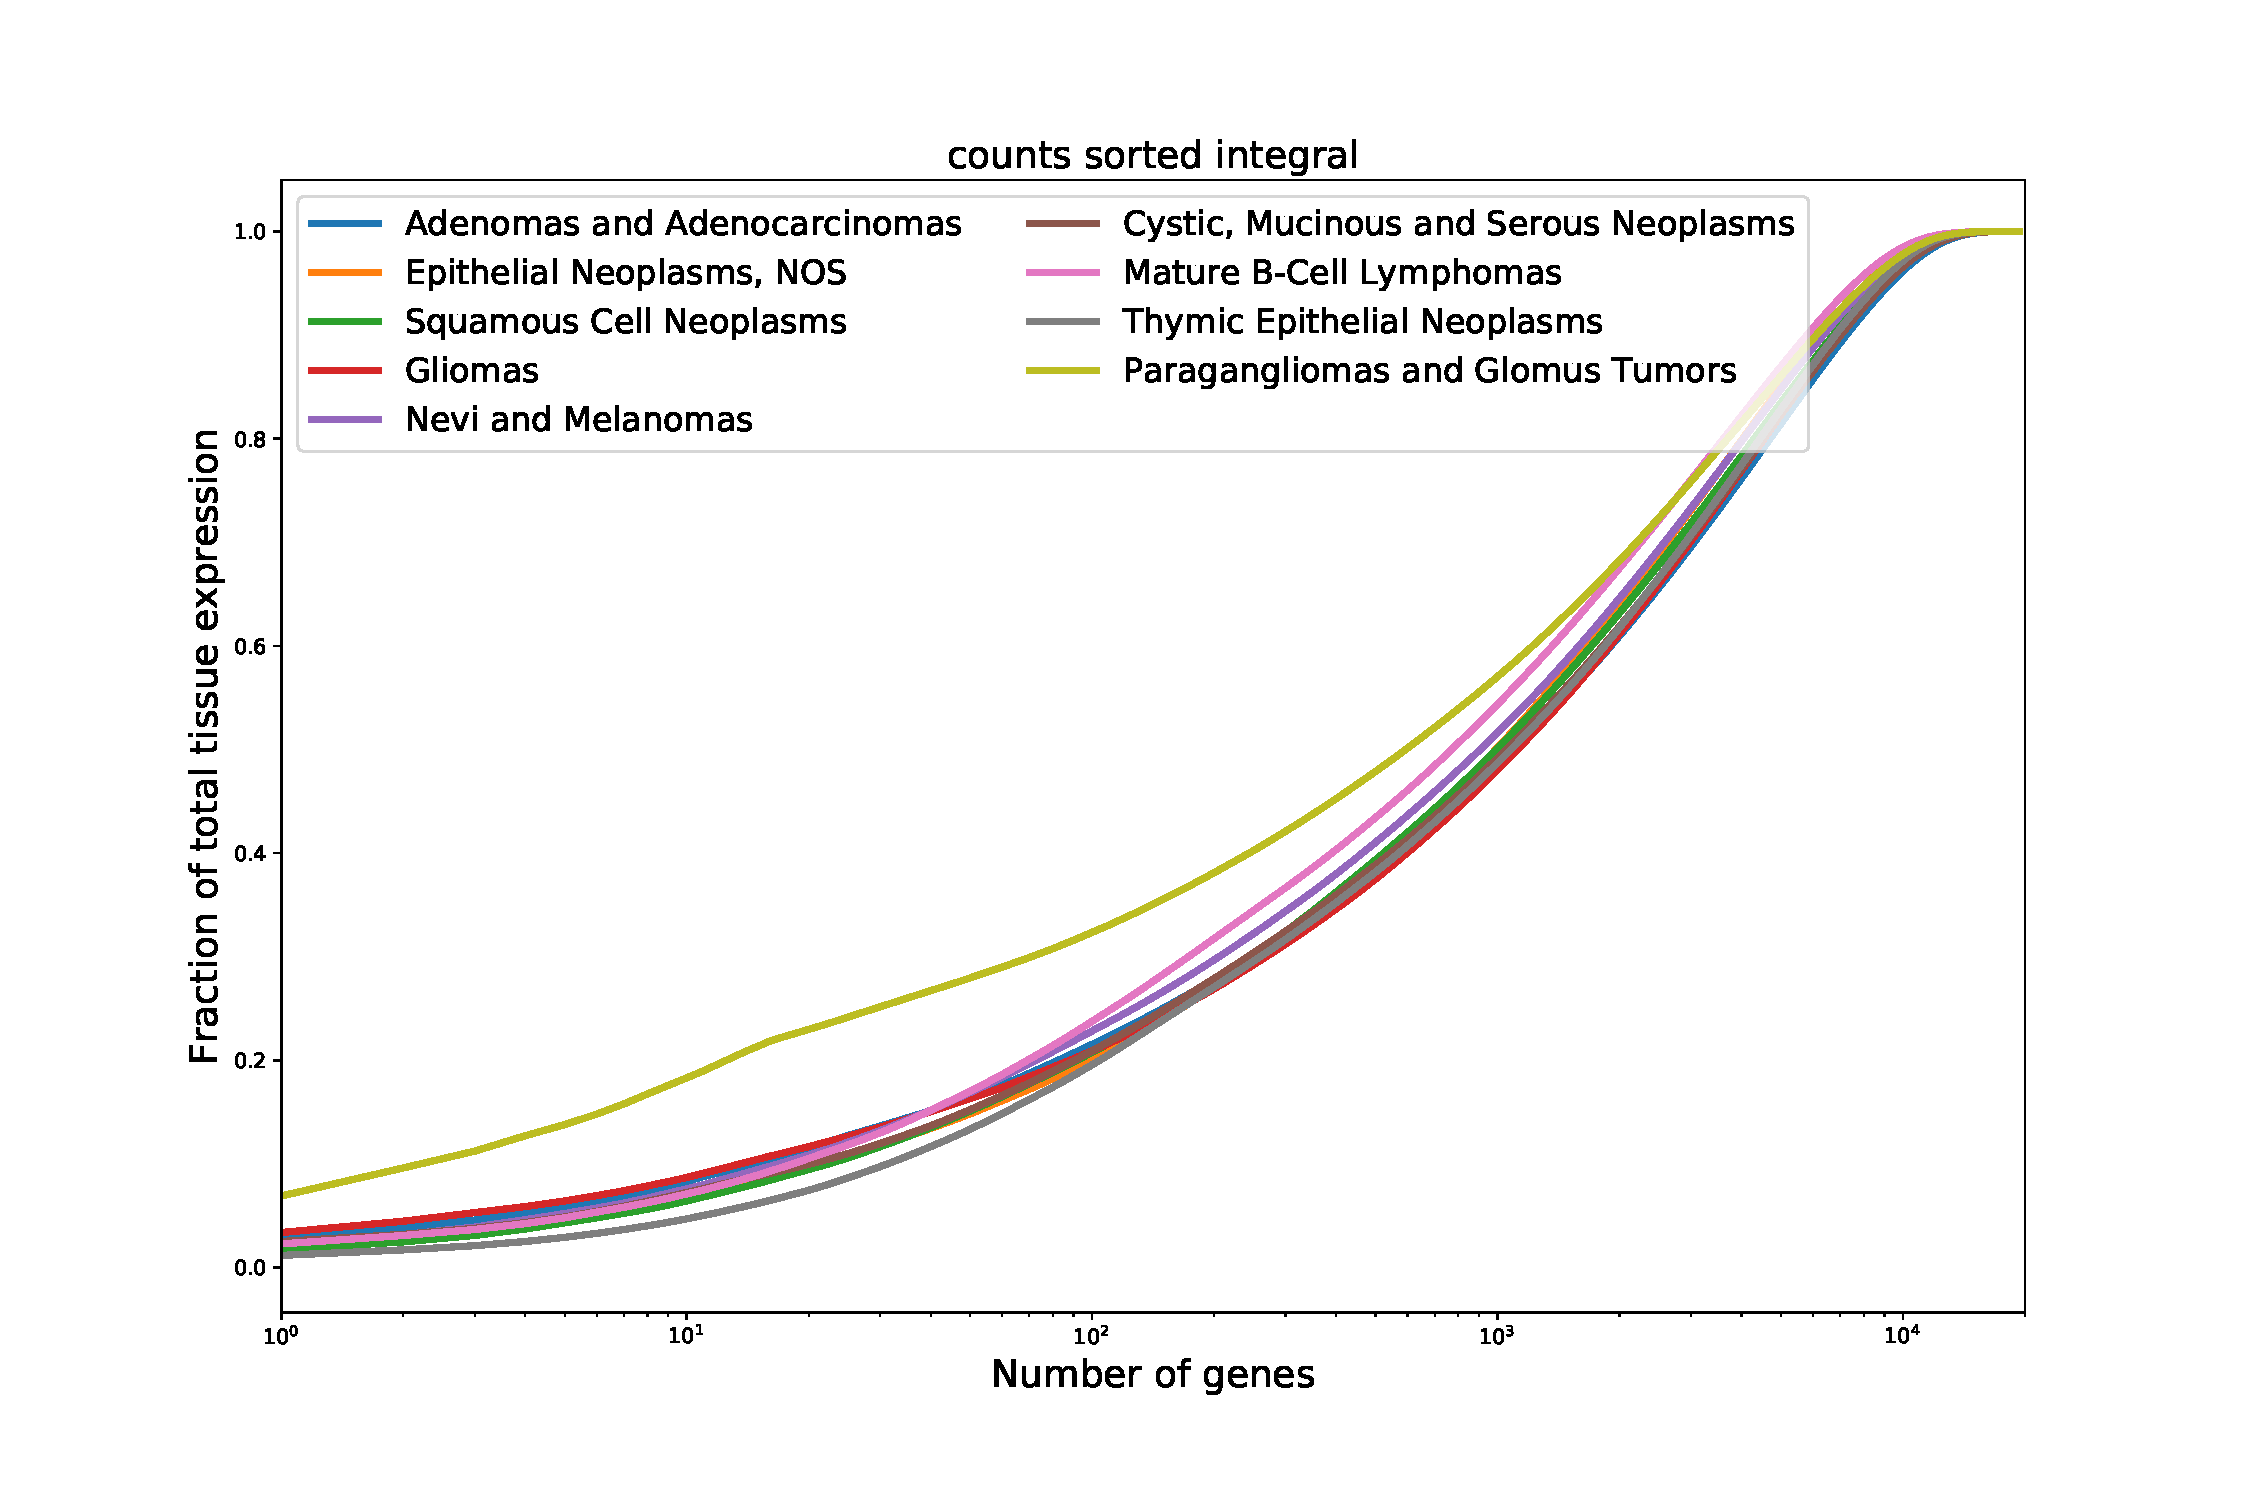
\includegraphics[width=0.8\linewidth]{pictures/structure/tcga/fraction_of_trascriptome_disease.pdf}
  \caption{The integral of the sorted abundances for each disease type.}
  \label{fig:structure/tcga/fraction_of_trascriptome_disease}
\end{figure}

\FloatBarrier
All these analyses suggest that there must be a sort of hidden structure in the data that is somehow related to the tissue each sample comes from. In particular, there are many Zipf's laws hidden behind the data and each sample is build looking at one of these a time. Also given two samples with a similar size, it happens that the number of genes necessary to build that realization is not always the same (shown by Heaps' law) and it is somehow related to the tissue of the sample.



\chapter{Scaling laws}\label{ch:scalinglaws}
One of the goals of this work is to search, reveal, study and use universal laws in bulk gene expression data~\nocite{altmann2016statistical}.
As in chapter~\ref{ch:structure} approaches from different field of science are considered at this point.

In can be interesting to study the behaviour of the gene expression across samples.

\section{Scaling}
\draft{gene expression across samples? gamma?}

Given a matrix of components and realisations as~\ref{fig:componetstable} with expression entries $n_{i j}$ it is possible to estimate the mean of a row $m_i=\avg{n_{i j}}_j$ and its variance $\var{i}=\avg{n_{i j}^2}_j - \avg{n_{i j}}^2_j$.

\paragraph{Variance versus mean}\mbox{}\\
First of all, it could be interesting to study the variance of expression $\var{\mathrm{counts}}$ versus its average $\avg{\mathrm{counts}}$ across tissues.
%%all genes
\begin{figure}[htb!]
    \centering
    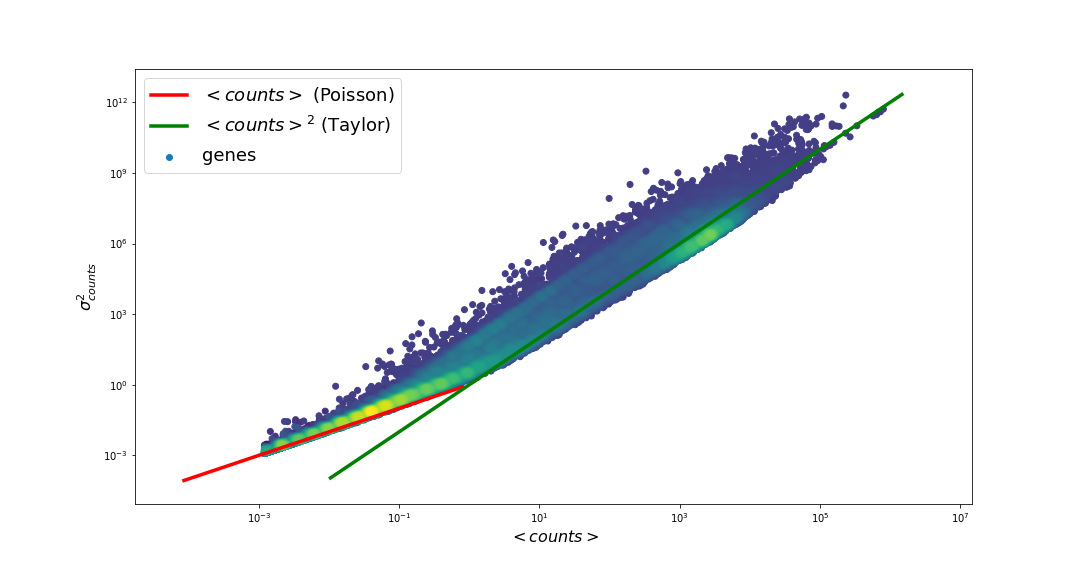
\includegraphics[width=0.9\linewidth]{pictures/scalinglaws/gtex/allgenes/varmean_loglog.png}
    \caption{Variance versus average. In \textcolor{pythonred}{red} the Poisson-like scaling, in \textcolor{pythongreen}{green} the Taylor-like scaling. All genes are considered.}
    \label{fig:scalinglaws/gtex/allgenes/varmean_loglog_density}
\end{figure}
In figure~\ref{fig:scalinglaws/gtex/allgenes/varmean_loglog_density} the scatter plot of variance versus mean reveals some interesting facts.
First of all, it is evident that data have a double scaling behaviour: when the mean is small ($\lesssim 1$) data scale a Poisson-like ($\var{\mathrm{counts}} \sim \avg{\mathrm{counts}}$), at higher means data present instead a quadratic scaling ($\var{\mathrm{counts}} \sim \avg{\mathrm{counts}}^2$) known in ecology as Taylor's law~\cite{Eisler2008}. This means that at low averages data's behaviour is due to the sampling process; on the contrary, Taylor's law reveals the non-trivial distribution across samples of the gene expression.

Another interesting fact is that looking at the density of points (colours in figure~\ref{fig:scalinglaws/gtex/allgenes/varmean_loglog_density}) two clouds of points emerge: one at low averages and one at high averages. These correspond to coding and non-coding genes, remembering section~\ref{sec:universallaws} these two kind of genes have different behaviours: protein-coding genes are highly expressed in the majority of the samples, non-coding ones are less expressed (and so less sampled) in a few samples. 

\paragraph{Coefficient of Variation}\mbox{}\\
A similar analysis, common in literature, is the analysis of the coefficient of variation squared $CV^2=\frac{\var{\mathrm{counts}}}{\avg{\mathrm{counts}}^2}$ represented in figure~\ref{fig:scalinglaws/gtex/allgenes/cvmean_loglog}.
\begin{figure}[htb!]
    \centering
    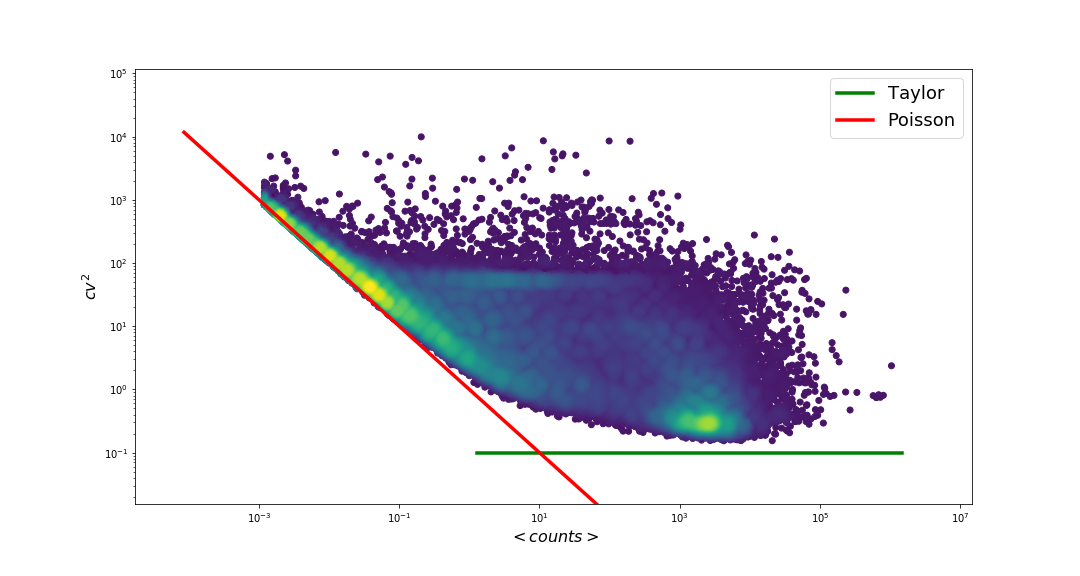
\includegraphics[width=0.95\linewidth]{pictures/scalinglaws/gtex/allgenes/cvmean_loglog.png}
    \caption{Coefficient of variation squared versus average. In \textcolor{pythonred}{red} the Poisson-like scaling, in \textcolor{pythongreen}{green} the Taylor-like scaling. All genes are considered.}
    \label{fig:scalinglaws/gtex/allgenes/cvmean_loglog}
\end{figure}
The behaviour is complementary to the one discussed above; a double scaling, quite common in the literature looking at single-cell RNA sequencing data~\cite{Islam2013}, is present. Even looking at $CV^2$ it is evident the presence of the protein-coding and non-coding clouds of points. The non-coding genes have a Poisson-like scaling, $\var{\mathrm{counts}} \sim \avg{\mathrm{counts}}$ so $CV^2=\frac{\var{\mathrm{counts}}}{\avg{\mathrm{counts}}^2}\sim\frac{1}{\avg{\mathrm{counts}}}$, otherwise the protein-coding genes are on the Taylor-like curve $CV^2=\frac{\var{\mathrm{counts}}}{\avg{\mathrm{counts}}^2}\sim \text{constant}$.

\paragraph{Protein-coding genes} can be isolated and considered on their own. The same analysis confirms that the cloud of points on the Taylor-like scaling is made by protein-coding genes.
\begin{figure}[htb!]
    \centering
    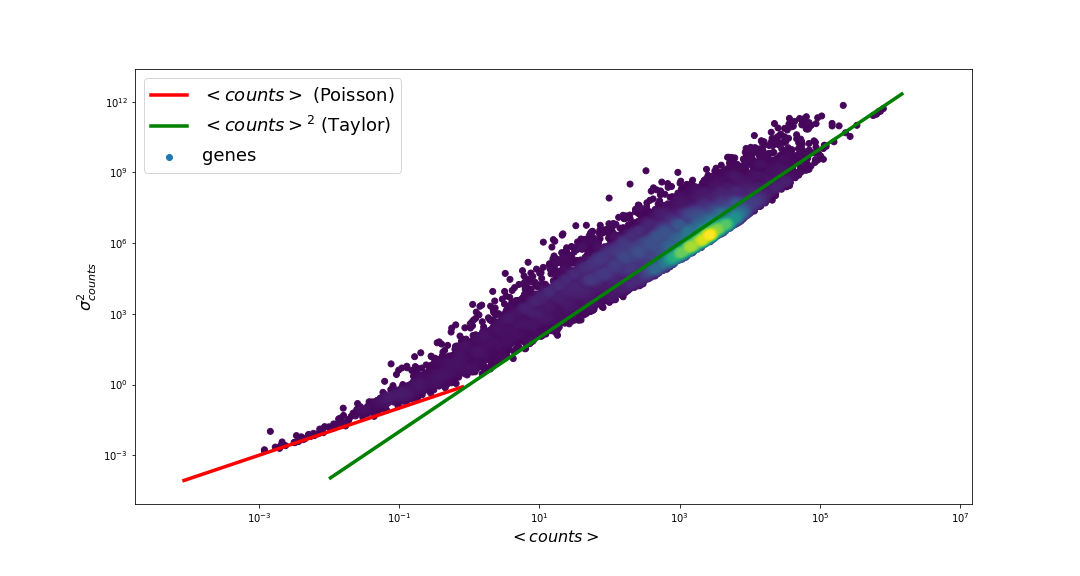
\includegraphics[width=0.95\linewidth]{pictures/scalinglaws/gtex/varmean_loglog_density.png}
    \caption{Variance versus average. In \textcolor{pythonred}{red} the Poisson-like scaling, in \textcolor{pythongreen}{green} the Taylor-like scaling. Only protein-coding genes are considered.}
    \label{fig:scalinglaws/gtex/varmean_loglog_density}
\end{figure}

Following the sampling model of~\cite{Mazzolini2018} summed up in section~\ref{sec:nullmodel} the averages and variances can be estimated on null matrices. In figure~\ref{fig:scalinglaws/gtex/varmean_3sigma} the comparison between real genes and sampling data. The sampling has got a double scaling as well; this is quite interesting, it means that the global scaling is due to the Zipf distribution and the sizes' distribution themselves, they are, by definition, identical in the data and in sampling.
Moreover, the sampling points draw a lower bound of the data, this encodes the information that the data are more variable (have higher variance) than just sampling, so there must be some biological information hidden that causes this over-variable behaviour.
\begin{figure}[H]
    \centering
    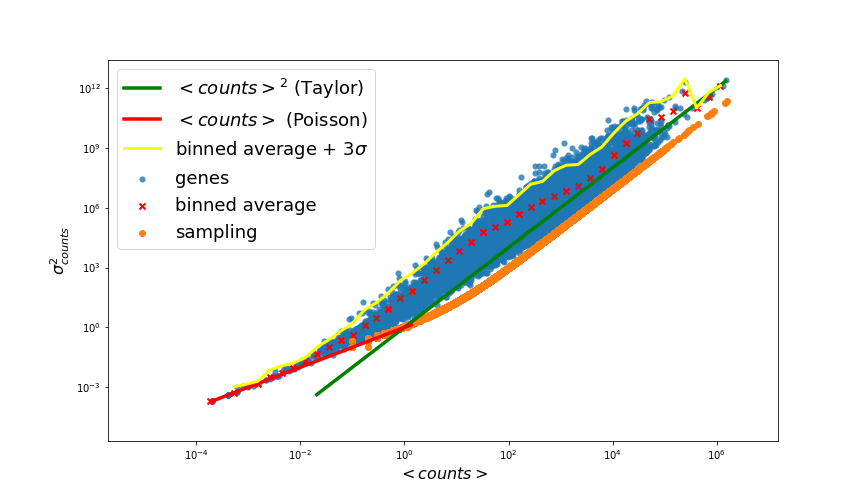
\includegraphics[width=0.8\linewidth]{pictures/scalinglaws/gtex/varmean_3sigma.png}
    \caption{Variance versus average. In \textcolor{pythonred}{red} the Poisson-like scaling, in \textcolor{pythongreen}{green} the Taylor-like scaling. In \textcolor{pythonorange}{orange} the sampling components. Only protein-coding genes are considered.}
    \label{fig:scalinglaws/gtex/varmean_3sigma}
\end{figure}

Again it is possible to analyse the $CV^2$, this time considering only protein-coding genes. Figure~\ref{fig:scalinglaws/gtex/allgenes/cvmean_loglog} confirms that the cloud of points near the Taylor-like scaling is made of protein-coding genes and a double scaling is seen once again.
\begin{figure}[htb!]
    \centering
    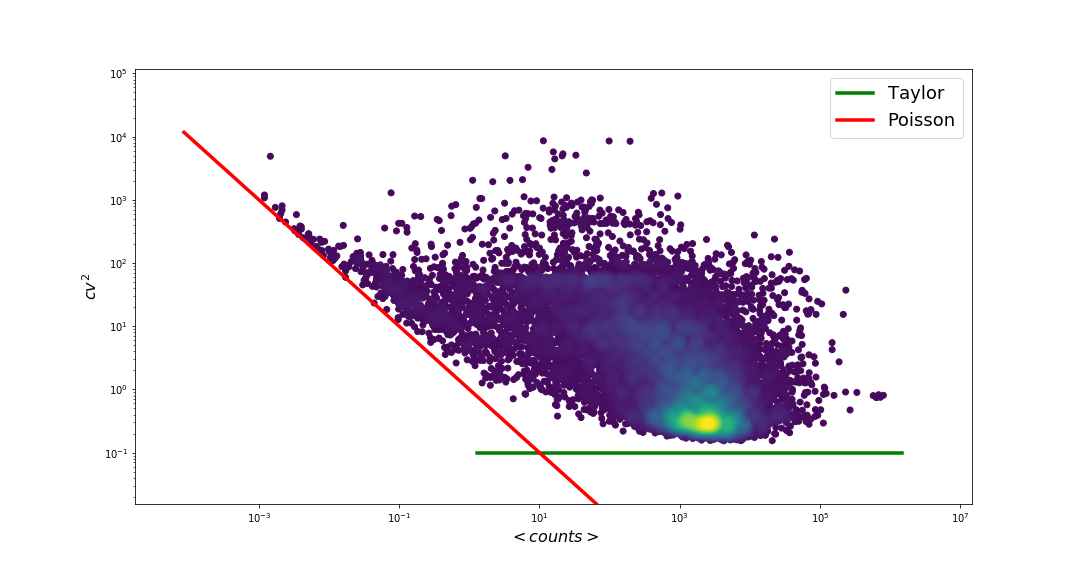
\includegraphics[width=0.9\linewidth]{pictures/scalinglaws/gtex/cvmean_loglog_density.png}
    \caption{Coefficient of variation squared versus average. In \textcolor{pythonred}{red} the Poisson-like scaling, in \textcolor{pythongreen}{green} the Taylor-like scaling. Only protein coding genes are considered.}
    \label{fig:scalinglaws/gtex/cvmean_loglog}
\end{figure}

In figure~\ref{fig:scalinglaws/gtex/cvmean_loglog_sampling} the same plot compared to the sampling data. The double scaling is evident also for the sampling points. Note that $CV^2$ has got a lower bound at $0$ which corresponds to the less variable case: all expressions are identical in all samples ($\var{\mathrm{counts}}=0$). There is an upper bound at $R-1$, with $R$ the number of realizations, that corresponds to the most variable case: a component expresses in only one realization and is $0$ elsewhere.
\begin{figure}[htb!]
    \centering
    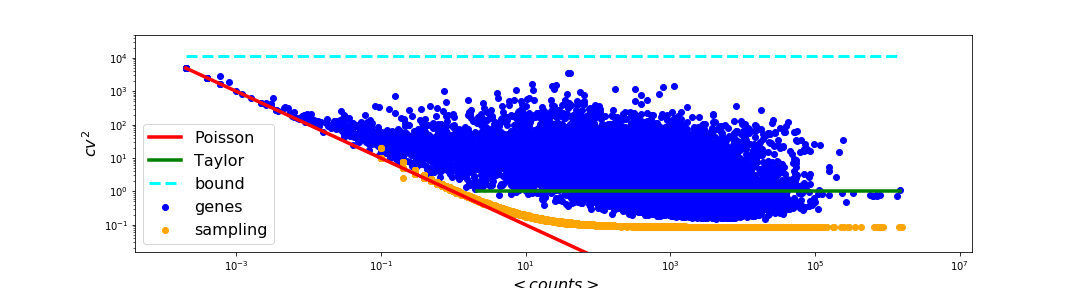
\includegraphics[width=0.9\linewidth]{pictures/scalinglaws/gtex/cvmean_loglog_sampling.png}
    \caption{Coefficient of variation squared versus average. In \textcolor{pythonred}{red} the Poisson-like scaling, in \textcolor{pythongreen}{green} the Taylor-like scaling. In \textcolor{pythonorange}{orange} the sampling components.}
    \label{fig:scalinglaws/gtex/cvmean_loglog_sampling}
\end{figure}

Finally, the data have a double scaling when looking at their global variance across realizations, a Poisson-like scaling in the region where the sampling experimental process is more important and a Taylor-like scaling where the complexity of the data emerges.
Non-coding genes have got low expression and are rare; protein-coding genes, otherwise, express a lot and everywhere and carry more information; this behaviour results in a double scaling. All genes are more variable than a sampling null model and this is the evidence that something interesting is hidden behind the data.


\paragraph{$<FPKM>$ normalisation}
One can be interested in finding genes that are expressed often, and what is the 
average expression of them.
To manage this it is plotted the average expression $<FPKM>$ versus the number 
of samples in which that gene is expressed that is, considering the thresholds~\ref{sec:threshold}, 
$\Sigma_j\theta (FPKM_{ij}-0,1)\theta (10^5-FPKM_{ij})$

\subsection{Average versus occurrence}
Another interesting analysis can be the relation between the occurrence and the average. In figure~\ref{fig:scalelaws/gtex/meanDiff_binned_sampling} it is shown the result, it is clear that there is a relation between occurrence and average, genes that express in more realisations (higher occurrence and right in the figure) have an higher average. Moreover doesn't exist genes that have high expression in few realisations; genes that are rare are also difficult to find so have a small average. Note that the average has got a bound due to the fact that counts are integer numbers, so if, for example, one gene express in $n$ of the $R$ samples, it has occurrence $O_i=\frac{n}{R}$ and its average is at least $\avg{\mathrm{counts}}=\frac{1*n}{R}$
\begin{figure}[htb!]
    \centering
    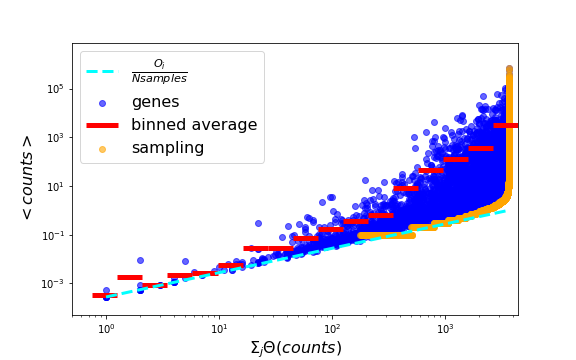
\includegraphics[width=0.9\linewidth]{pictures/scalelaws/gtex/meanDiff_binned_sampling.png}
    \caption{Relation between the occurrence of a gene and its average across realisations}
    \label{fig:scalelaws/gtex/meanDiff_binned_sampling}
\end{figure}

\subsection{Tissue differentiation}
Per gene type scaling




\chapter{Topic modelling}\label{ch:topicmodelling}
Once extensively analysed the structure of the dataset, the goal becomes to develop a machine learning method to learn the hidden structure of the data.  
%%intro
Remembering that in chapter~\ref{ch:structure} it emerged some kind of structure behind data, where each tissue seemed to be sampled by a different power law, a topic modelling approach is here proposed. Topic modelling has been developed and studied to approach linguistics problems, so this algorithm was developed considering words and books in input, links represent the abundance of a word in a book. In chapter~\ref{ch:structure} was evident that there are many similarities between data considered in this work and linguistics' corpora. Referring to data used in this project \textbf{samples} will be the documents and \textbf{genes} will be the words. It is expected that topics represent some properties of the system due to the gene expression distribution in samples.

The idea is that behind data there are hidden variables that describe the relationship between the genes and the samples. Let's call these variables topics.
Firstly it is necessary to build a bipartite network of genes and samples, then nodes are linked considering the gene expression value in the dataset.
\begin{figure}[htb!]
    \centering
    \includegraphics[width=0.7\linewidth]{pictures/topic/bipartite.pdf}
    \caption{An example of a bipartite network. Samples are on the left, genes are on the right. Each link is weighted by gene expression value. On the left side, all nodes of the same colour are clusters of samples. On the right side, all nodes with the same colour are a set of genes, also known as topics.\\
    Blue lines represent the cluster structure, each blue squared-dot is a set of nodes, lines delineate the hierarchical structure.\\
    It is clear in the middle the network separation between genes and samples.}
    \label{fig:topic/bipartite}
\end{figure}

The output of this kind of models consists of sets of genes, the topics, with a probability distribution $P(\text{gene} | \text{topic})$ and probability distributions of these topics inside each sample $P(\text{topic} | \text{sample})$, together they give the relationship between a \textit{sample} and a \textit{gene}.

In this work, an innovative and recent approach to topic model is proposed. The algorithm was presented by~\cite{gerlach2018network} and~\cite{Peixoto2017} explain it in details. This model is an evolution of a stochastic block model~\cite{Holland1983}. It is called hierarchical Stochastic Block Model (hSBM).

The ultimate goal is to be able to separate healthy and diseased samples then find and separate well-known tumour types and finally extend the actual knowledge and retrieve the tumour sub-types.

One of the advantages of this particular algorithm is that it is hierarchical, so it applies community detection at different layers of resolution. So the output has got different resolutions and different number of clusters at each layer . One extreme layer is the one which separates genes ($\simeq$ words) and samples ($\simeq$ samples), by definition; in other layers, it is possible to have few big clusters until the other extreme were the number of clusters is comparable with the number of nodes.
\begin{figure}[htb!]
  \centering
  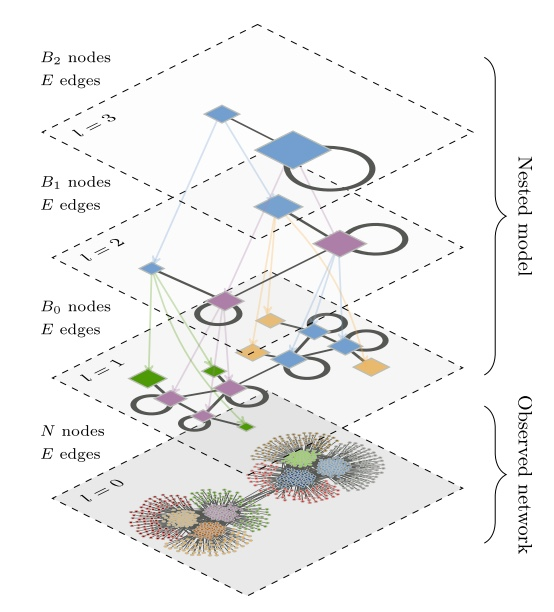
\includegraphics[width=0.6\linewidth]{pictures/topic/peixioto_hierarchic.jpg}
  \caption{Example of a hierarchical structure. At $l=0$ the number of cluster is comparable with the number of nodes, is the situation with many small clusters. Then they're merged in bigger clusters at other layers of the hierarchy.}
  \label{fig:topic_peixioto_hierarchic}
\end{figure}

What the algorithm does is to run a sort of Monte Carlo simulation and find the best partition of the data.
The probability that the hidden variables $\theta$ describe the data $G$ $P(\theta | G)$ can be written as a likelihood times a prior probability as
\[P(\theta|G)=\frac{P(G|\theta)\overbrace{P(\theta)}^{prior}}{\underbrace{P(G)}_{\sum_{\theta}P(G|\theta)P(\theta)}}.\]
It is possible to define a description length
\[
\Sigma=-lnP(G|\theta)-lnP(\theta),
\]
so that $P(\theta | G)\propto e^{-\Sigma}$.
Moreover, the likelihood $P(G | \theta)$, can be written as $\frac{1}{\Omega}$ where $\Omega(\theta)$ is the number of networks that is possible to build given $\theta$. This corresponds to a microcanonical ensemble with entropy $S=Ln\left(\Omega\right)$. According to~\cite{peixoto2017nonparametric} entropy $S$ can be written as
\[
S=\frac{1}{2}\Sigma_{r,s} n_r n_s H\left(\frac{e_{rs}}{n_rn_s}\right),
\]
where $n_r$ is the number of nodes in the block $r$, $e_{rs}$ the number of links between nodes of group $r$ and nodes of group $s$ and $H$ is the Shannon entropy $H(x)=xLog_2(x)+(1-x)Log_2(1-x)$. Note that $S$ is minimal if $\frac{e_{rs}}{n_rn_s}$ is close to zero, $r$ and $s$ are two completely separated blocks or if it is close to $1$, $r$ and $s$ are groups with many connections; this allows finding groups with nodes very disconnected or topic and clusters with a lot of connections. Note that the description length depends on the entropy:
\[
\Sigma=S-lnP(\theta),
\]
The algorithm tries to minimize $S$, so that $\Sigma$ is minimized, so $e^{-\Sigma}$ is maximized, but this is $P(\theta | G)$ that is the required probability to maximize.

The Monte Carlo simulation works in a few steps:
\begin{itemize}
 \item a node $i$ is chosen,
 \item the group of $i$ is called $r$,
  \item a node $j$ is chosen from $i$'s neighbours, the group of $j$ is called $t$,
  \item a random group $s$ is selected,
  \item move of node $i$ to group $s$ is accepted with probability $P(r\to s|t)=\frac{e_{ts}+\epsilon}{e_t+\epsilon B}$,
  \item if the move to $s$ is not accepted, a random edge $e$ is chosen from group $t$ and node $i$ is assigned to the endpoint of $e$ which is not in $t$;
\end{itemize}
in figure~\ref{fig:topic_peixioto_move} an example of these steps.
\begin{figure}[htb!]
  \centering
  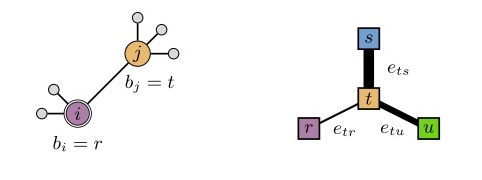
\includegraphics[width=0.9\linewidth]{pictures/topic/peixioto_move.jpg}
  \caption{Left: Local neighbourhood of node $i$ belonging to block $r$, and a randomly chosen neighbour $j$ \
  belonging to block $t$. \
  Right: Block multi-graph, indicating the number of edges between blocks, represented as the edge thickness. \
  In this example, the attempted move $bi \to s$ is made with a larger probability than either $bi \to u$\
   or $bi \to r$ (no movement), since $e_{ts}>e_{tu}$ and $e_{ts}>e_{tr}$.}
  \label{fig:topic_peixioto_move}
\end{figure}

In order to remove eventual biases due to the initial configuration the model is run with $5$ different initial states, then the final state with the minimal entropy is selected.

Once the model run it is possible to estimate the probability distribution of words inside a topic
\[P(w|t_w)=\frac{\text{\# of edges on $w$ to $t_w$}}{\text{\# of edges on $t_w$}}\]
and the topic distribution inside a document
\[P(t_w|d)=\frac{\text{\# of edges on $d$ from $t_w$}}{\text{\# of edges on $d$}}\]
This algorithm can set to have overlapping partitions; in this case, the presence of a word in a topic is not trivial and can be estimated as
\[P(t_w|w)=\frac{\text{\# of edges on $w$ to $t_w$}}{\text{\# of edges on $w$}}\]
or the presence of a document in a cluster
\[P(t_d|d)=\frac{\text{\# of edges on $d$ to $t_d$}}{\text{\# of edges on $d$}}\]

See appendix~\ref{app:hsbm} for a detailed analysis of the maths behind the algorithm and \url{https://cloud.docker.com/repository/docker/fvalle01/hsbm} for the extension of~\cite{gerlach2018network} to non-linguistics component systems datasets.


%%metrics
\section{Metrics and benchmarks}
Before running topic modelling, it is useful to define some metrics to test and benchmark the model. In particular the model searches sets on the two sides of the network the one containing samples and the one containing genes. Samples are extracted from datasets where much metadata are available, some of these metadata labels will be used to benchmark the model. To study genes enrichment test are necessary.

Looking at the samples side of the network, the outputs are sets of samples, the clusters. One can state the model works if all, or at least the majority, of samples in the same cluster share some label. Here the tissue is considered as the main label.

Note that this work's model is a non supervised one, but a ground truth is available from metadata. So every sample has a certain probability to have a certain property (the true tissue label), let's call this $P(C)$ and a certain probability of being in a cluster (model's output), let's call this $P(K)$.
It is possible to define some quantities, the homogeneity
\begin{equation}\label{eq:homogeneity}
    h=1-\frac{H(C|K)}{H(C)}
\end{equation}
defining the entropy
\begin{equation}\label{eq:hck}
    H(C|K)=\sum_{c\in \mathrm{tissues},\\ k \in \mathrm{clusters}}\frac{n_{c k}}{N}Log\left(\frac{n_{c k}}{n_k}\right)
\end{equation}
where $n_{c k}$ is the number of nodes of type $c$ in cluster $k$, $N$ the number of nodes and $n_k$ the number of nodes in cluster $k$. It is evident that if all nodes inside cluster $k$ are of the same type $c$ $n_{c k}=n_{k}$, $H(C|K)=0$ and $h=1$, it is actually a complete homogeneous situation.

Another quantity can be defined: the so-called completeness
\begin{equation}\label{eq:completness}
    c=1-\frac{H(K|C)}{H(K)},
\end{equation}
$H(K|C)$ is defined in the same way as~\ref{eq:hck}. Completeness measures how well nodes of the same type are distributed in the same cluster.

Ideally one wants a method which output is both homogeneous and complete. So it is possible to define the V-measure as the harmonic average of the two:
\begin{equation}\label{eq:mutualinformation}
    \mathrm{V-measure}=2\frac{h c}{h + c},
\end{equation}
which is actually the normalized mutual information between $P(C)$ and $P(K)$~\cite{rosenberg2007v}. Please refer to appendix~\ref{app:vmeasure} for the detailed maths. In figure~\ref{fig:topic/metric_scores_primarysite} an example of the V-measure score estimated at the different layers of the hierarchy; note that the number of clusters increases going deeper in the hierarchy. In the same figure homogeneity and completeness are reported, note that with few clusters the situation is more complete, but when the number of clusters increases completeness goes down and homogeneity increases. 
\begin{figure}[htb!]
    \centering
    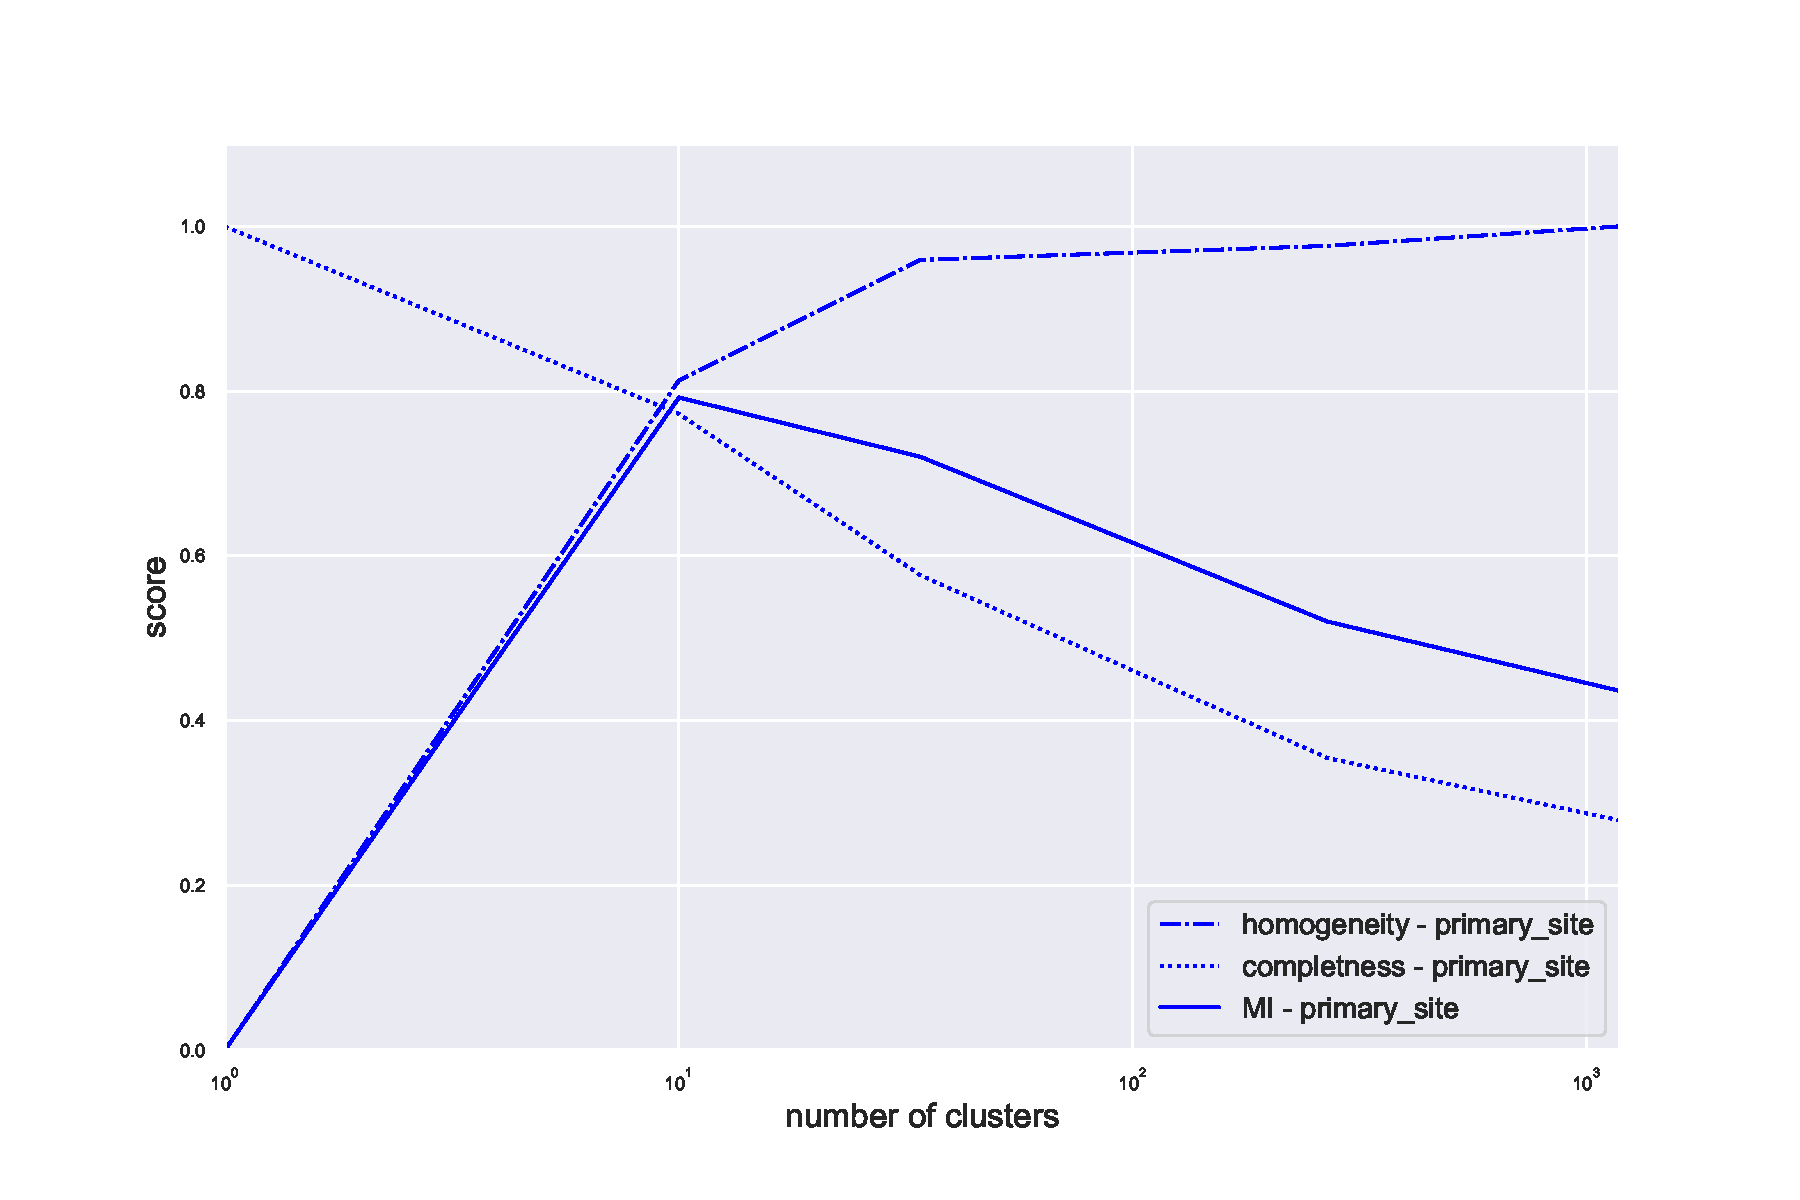
\includegraphics[width=0.8\linewidth]{pictures/topic/gtex/oversigma_10tissue/metric_scores_primarysite.pdf}
    \caption{Score across hierarchy. The V-measure or normalized mutual information MI is the harmonic average between homogeneity and completeness.}
    \label{fig:topic/metric_scores_primarysite}
\end{figure}

In the next sections will be studied also the maximum fraction of label in the same cluster defined as 
\[\mathrm{max}_{c\in k}\frac{n_{c k}}{n_k}.\] Also the number of different labels in the same cluster will be studied.
\FloatBarrier

%%preprocess
\section{Pre-process}
To make the algorithm faster, it could be useful to do a pre-processing of the data.
Different approaches were tested, all of them involving the quantities defined in~\ref{ch:structure}. The goal is to identify components which are able to best separate the realizations. 
\paragraph{Low occurrence genes} were selected firstly to approach topic modelling. A $0.5$ threshold was set on occurrence. This method selects genes that appears (have expression greater than zero) only in less than half samples. This approach has some limitations, for instance it doesn't consider genes that appear everywhere (with occurrence $\simeq 1$) but changes their behaviour across realisations.

\paragraph{tf-idf (term frequency–inverse document frequency)} should help. This approach doesn't take in account original expression values $n_{ij}$, but a transformed version
\[
n^{new}_{ij}=\frac{n_{i j}}{M_j}\times \left(1-Log\left(o_i\right)\right)
\] which increases the importance of components with small occurrence $o_i$. This approach doesn't actually select components, which is still an issue.

\paragraph{Highly variable} genes can be selected. This is done using the $CV^2$ analysis done in chapter~\ref{ch:scalinglaws}.
\begin{figure}[htb!]
    \centering
    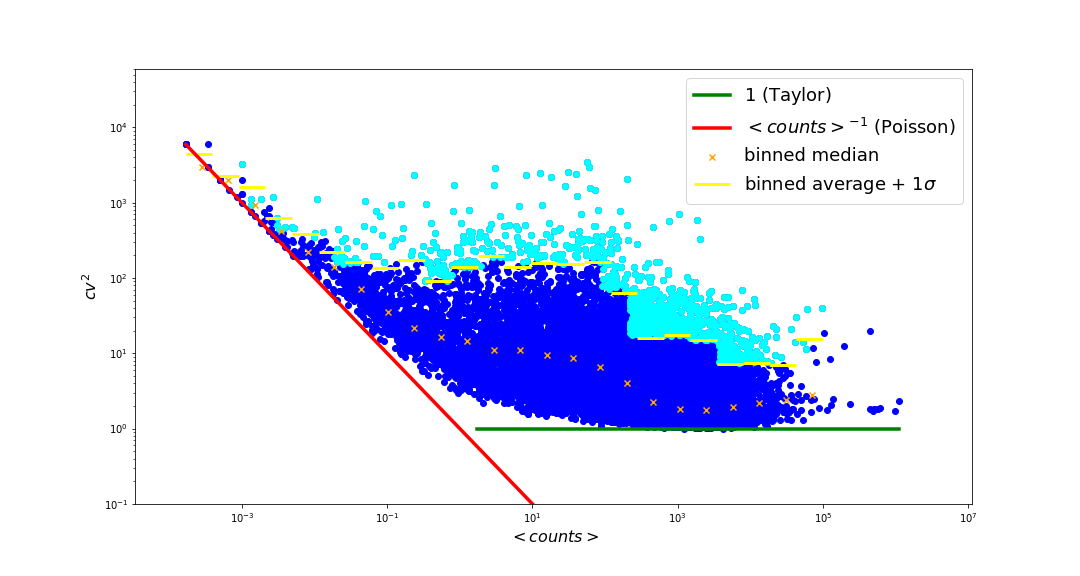
\includegraphics[width=0.8\linewidth]{pictures/topic/cvmean_oversigma.png}
    \caption{Highly variable genes}
    \label{fig:topic/cvmean_oversigma}
\end{figure}
Plotting the coefficient of variation versus the mean for each component reveals which components have higher variance with respect to components which, on average, have a similar behaviour. Binned averages and variances were estimated, and only genes with a $CV^2$ over a $\sigma$ greater than the bin's mean were considered. This method seems to select useful genes even if the binned average bound is quite noisy.

\paragraph{Distance from boundaries} can be a similar and alternative method to select highly variable genes. In this case the bound is smooth and well defined.
\begin{figure}[htb!]
    \centering
    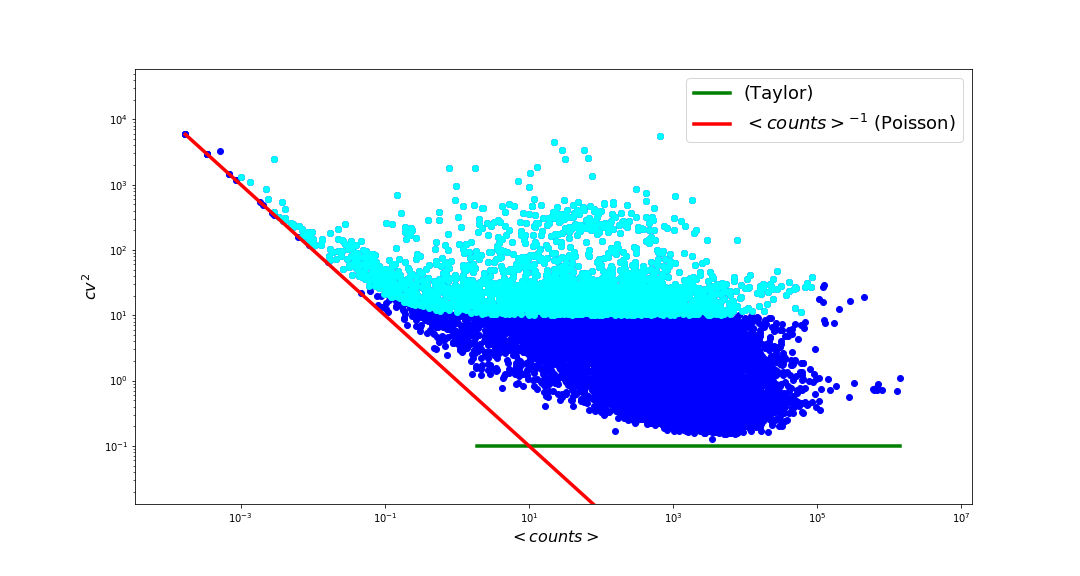
\includegraphics[width=0.8\linewidth]{pictures/topic/cvmean_oversampling.png}
    \caption{Genes distant from the boundaries}
    \label{fig:topic/cvmean_oversampling}
\end{figure}
The distribution as discussed in~\ref{ch:scalinglaws} have a Poisson-like and a Taylor-like boundaries. So can be considered only components that are the most distant from these boundaries. Moreover this boundaries can be found with a simple null model, as shown in figure~\ref{fig:scaling/gtex/cvmean_loglog_sampling} the sampling model defines the lower bound of the data.

The last two approaches are the ones which lead to better results, in the following sections gene selection was done by getting only highly variables genes.

\section{Run on GTEx}
\draft{Firstly the algorithm is run on a subset of $5$ tissues of GTEx}
\draft{metti 5 tissues?}
\begin{figure}[htb!]
    \centering
    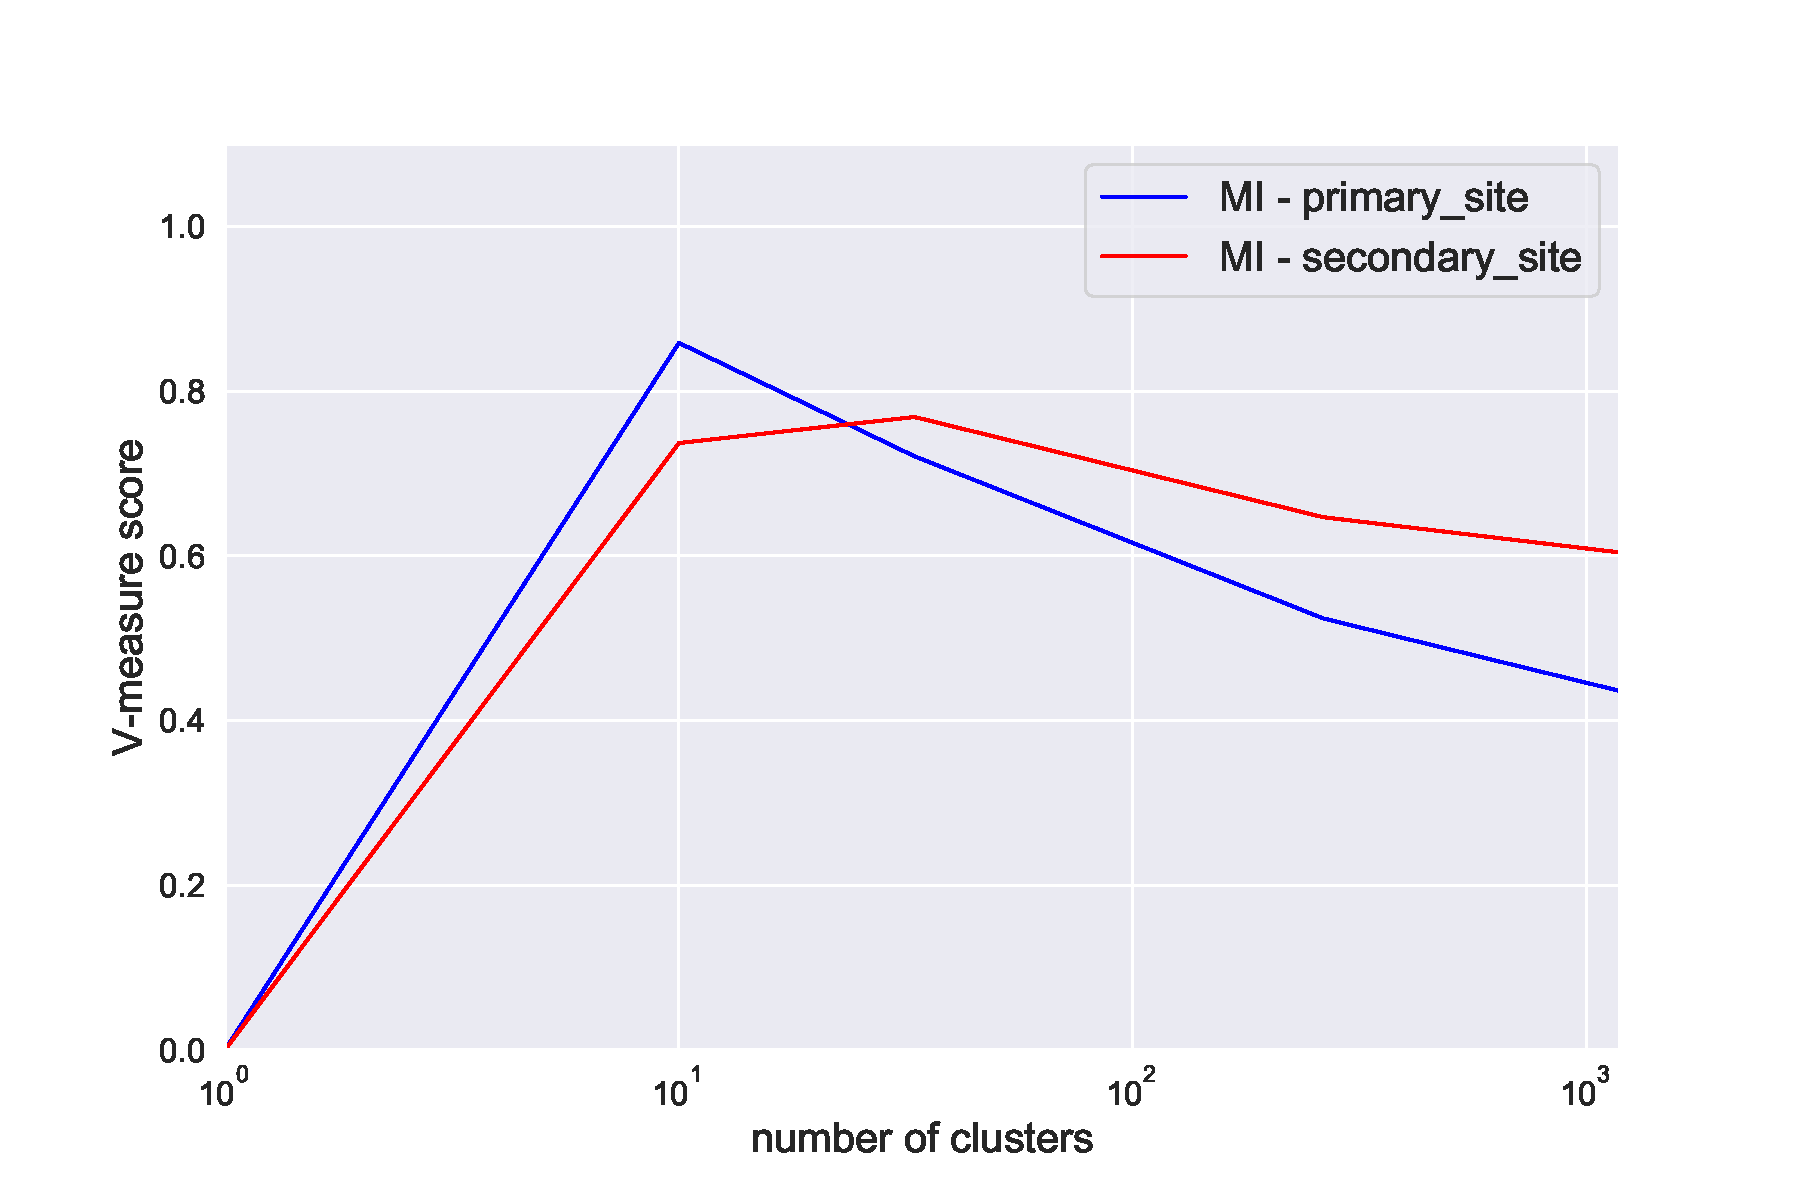
\includegraphics[width=0.9\linewidth]{pictures/topic/gtex/oversigma_10tissue/metric_scores.pdf}
    \caption{Scores accross hierarchy}
    \label{fig:my_label}
\end{figure}

\begin{figure}[htb!]
    \centering
    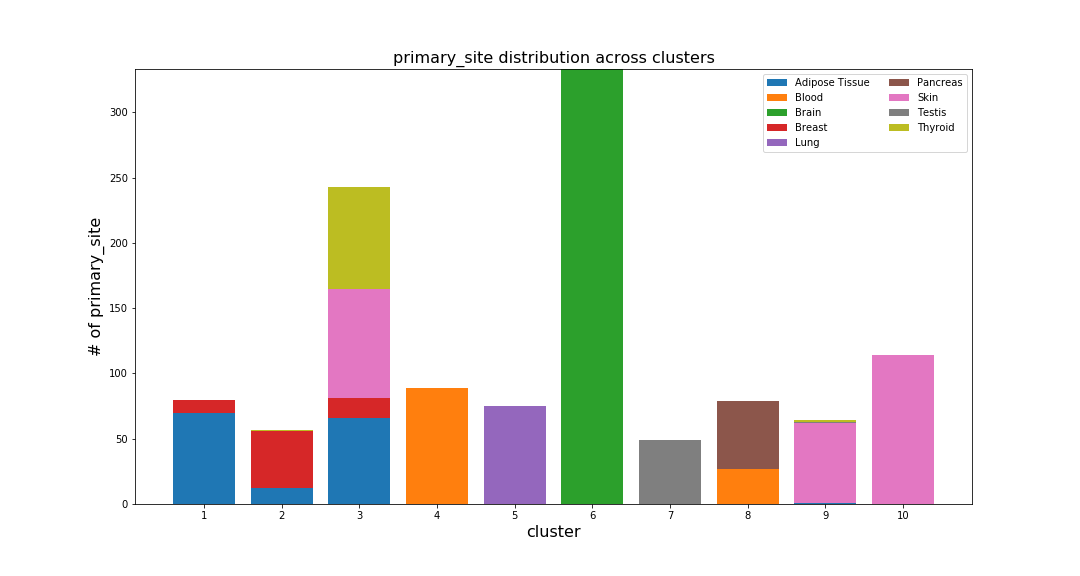
\includegraphics[width=0.9\linewidth]{pictures/topic/gtex/oversigma_10tissue/clustercomposition_l3_primary_site.png}
    \caption{Caption}
    \label{fig:topic/gtex/oversigma_10tissue/clustercomposition_l2_primary_site}
\end{figure}

\begin{figure}[htb!]
    \centering
    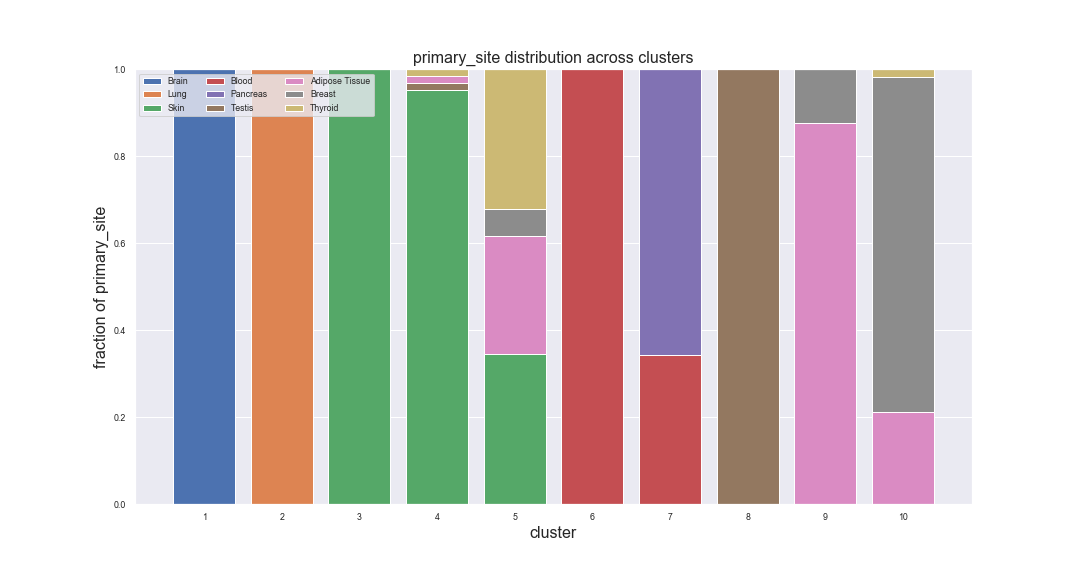
\includegraphics[width=0.9\linewidth]{pictures/topic/gtex/oversigma_10tissue/fraction_clustercomposition_l3_primary_site.png}
    \caption{Caption}
    \label{fig:topic/gtex/oversigma_10tissue/fraction_clustercomposition_l2_primary_site}
\end{figure}

\begin{figure}
    \centering
    \begin{minipage}{0.45\textwidth}
    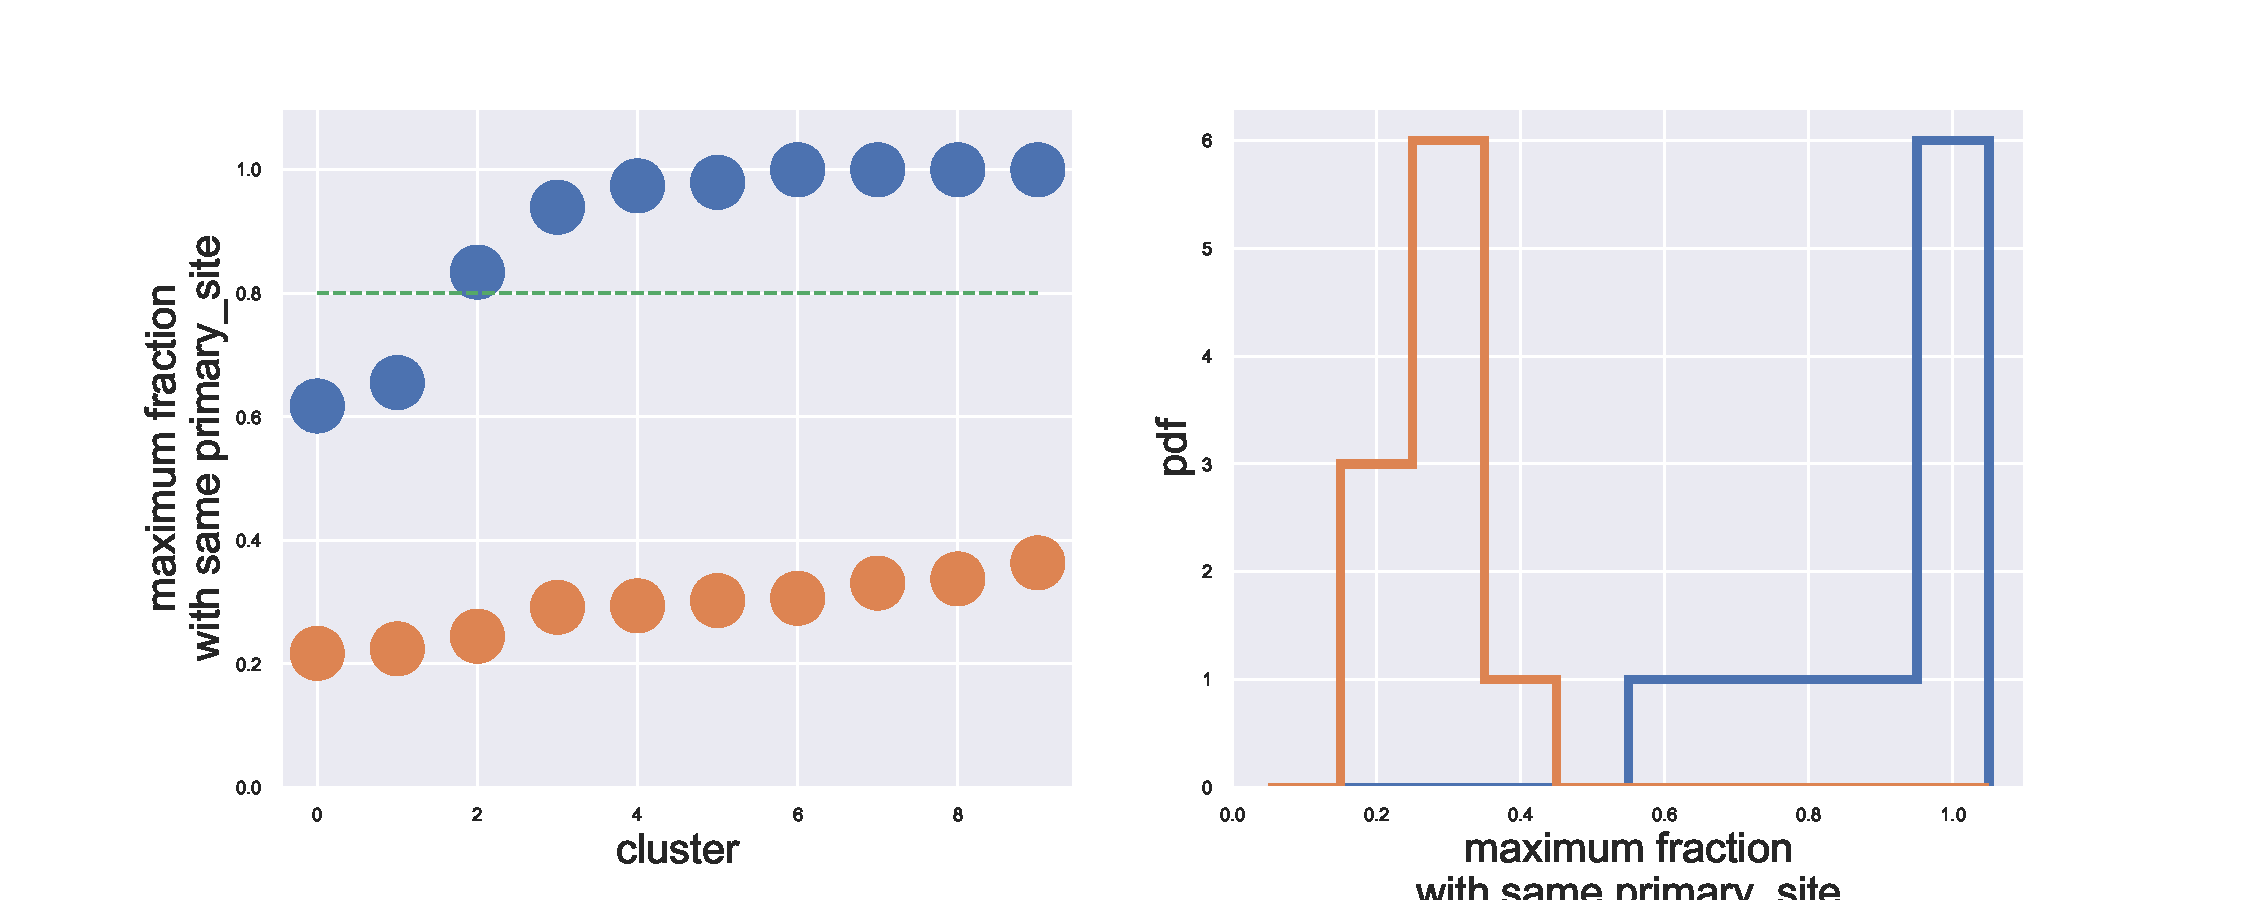
\includegraphics[width=0.9\linewidth]{pictures/topic/gtex/oversigma_10tissue/shuffledcluster_maximum_l3_primary_site.pdf}
    \end{minipage}
    \hspace{3mm}
    \begin{minipage}{0.45\textwidth}
    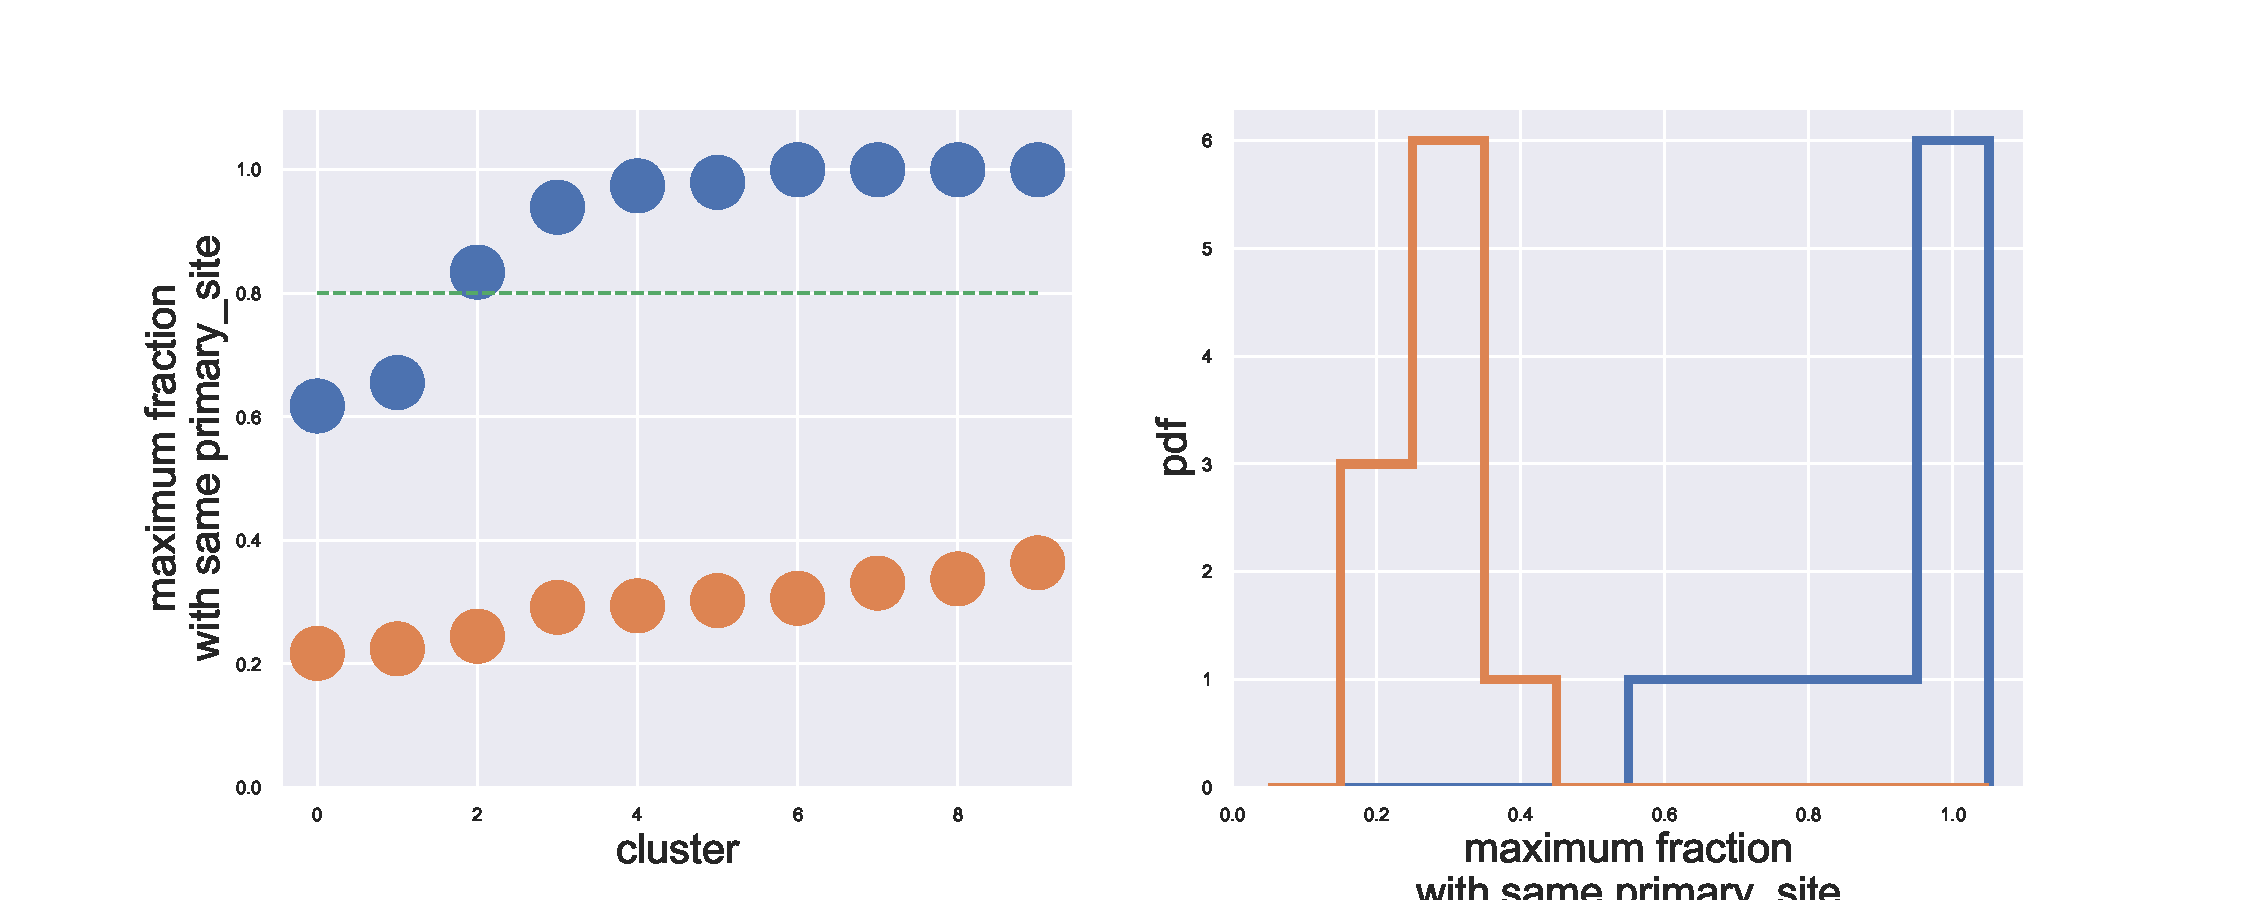
\includegraphics[width=0.9\linewidth]{pictures/topic/gtex/oversigma_10tissue/shuffledcluster_maximum_l3_primary_site.pdf}
    \end{minipage}
    \\
    \begin{minipage}{0.45\textwidth}
    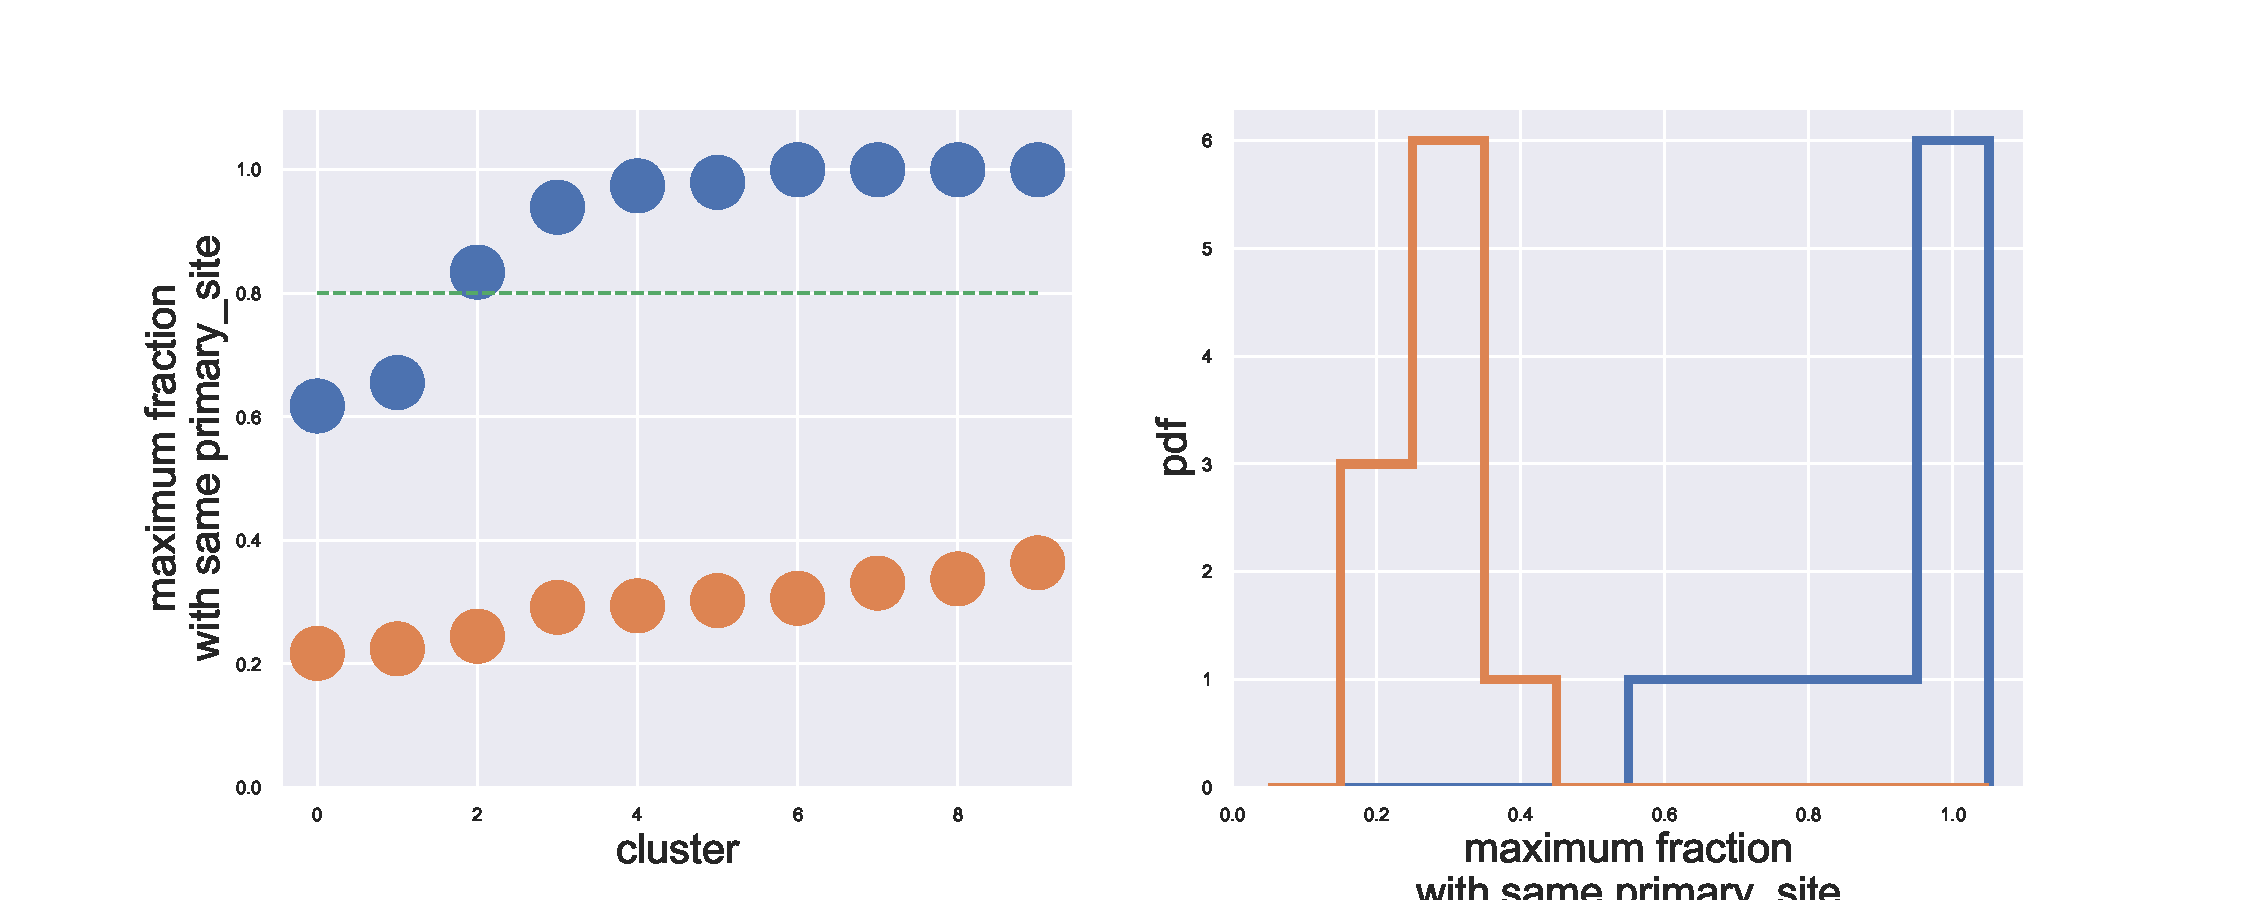
\includegraphics[width=0.9\linewidth]{pictures/topic/gtex/oversigma_10tissue/shuffledcluster_maximum_l3_primary_site.pdf}
    \end{minipage}
    \hspace{3mm}
    \begin{minipage}{0.45\textwidth}
    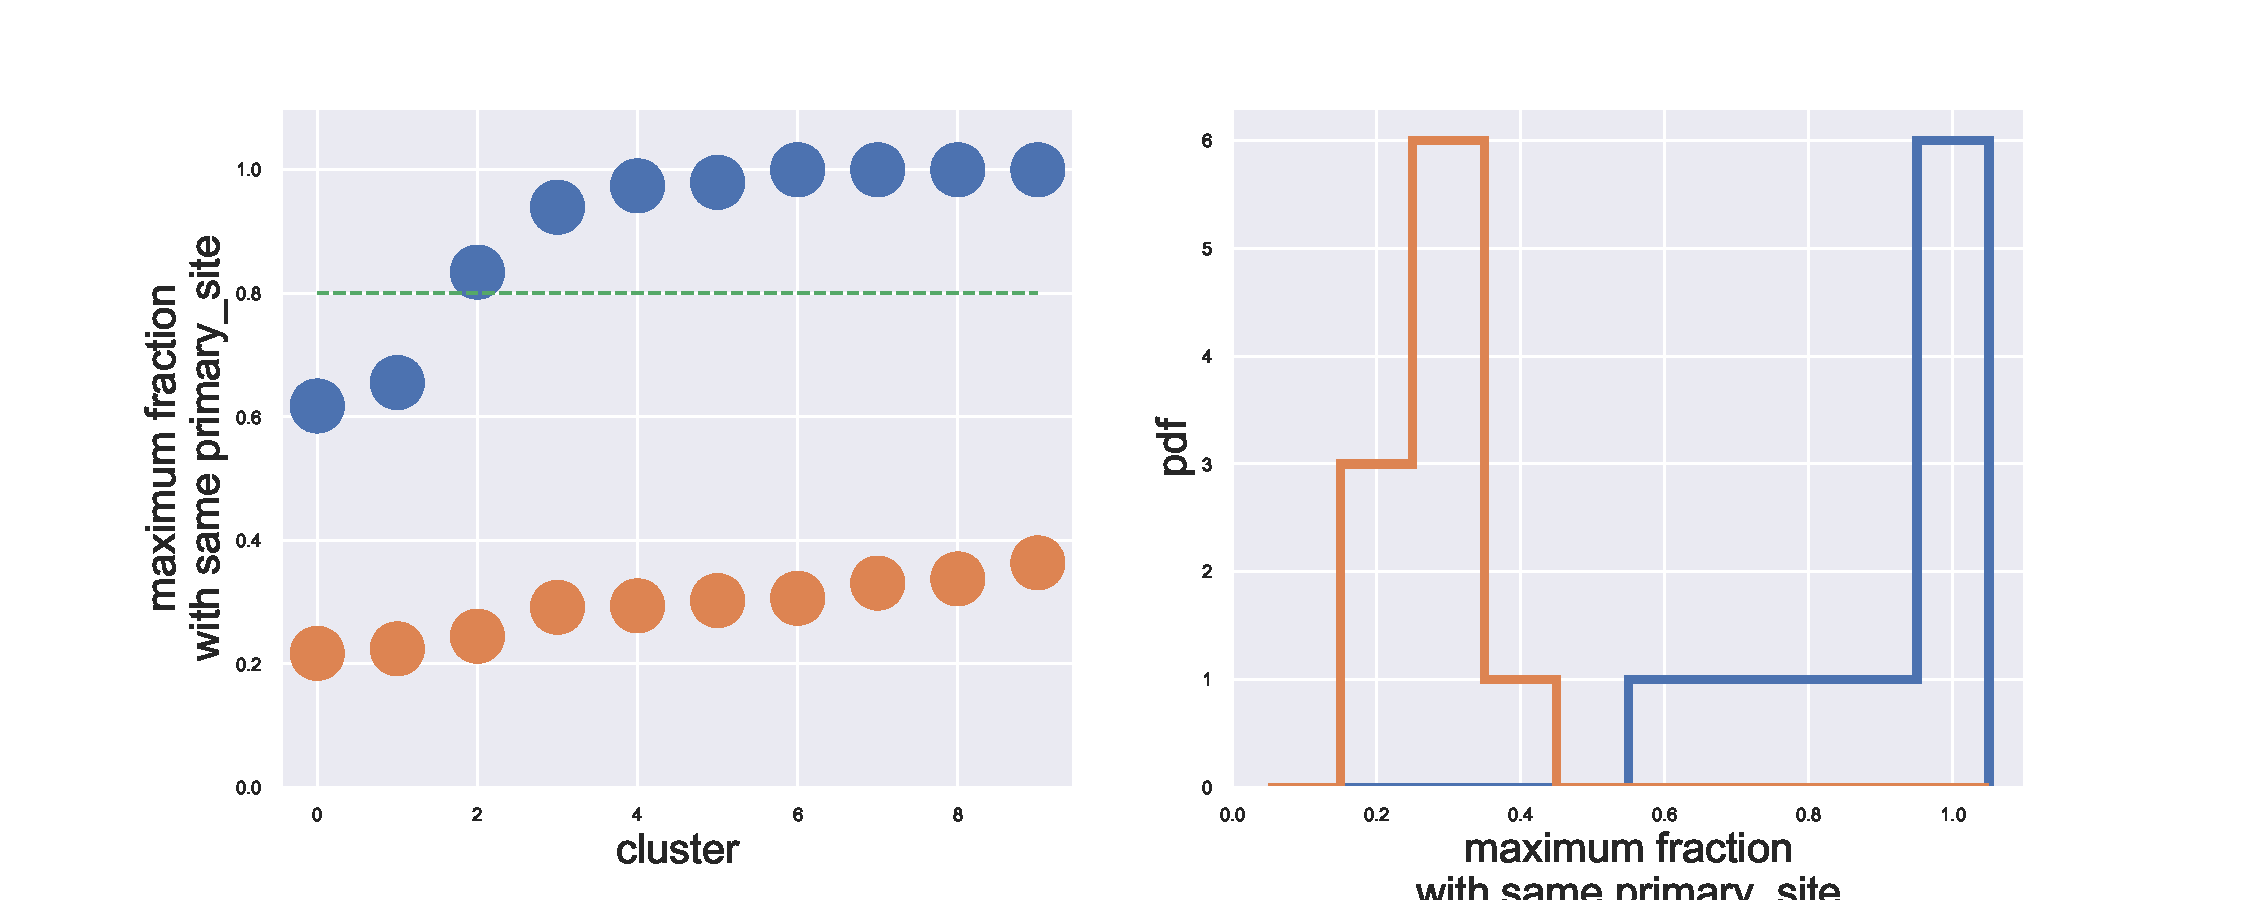
\includegraphics[width=0.9\linewidth]{pictures/topic/gtex/oversigma_10tissue/shuffledcluster_maximum_l3_primary_site.pdf}
    \end{minipage}
\end{figure}


\begin{figure}[htb!]
    \centering
    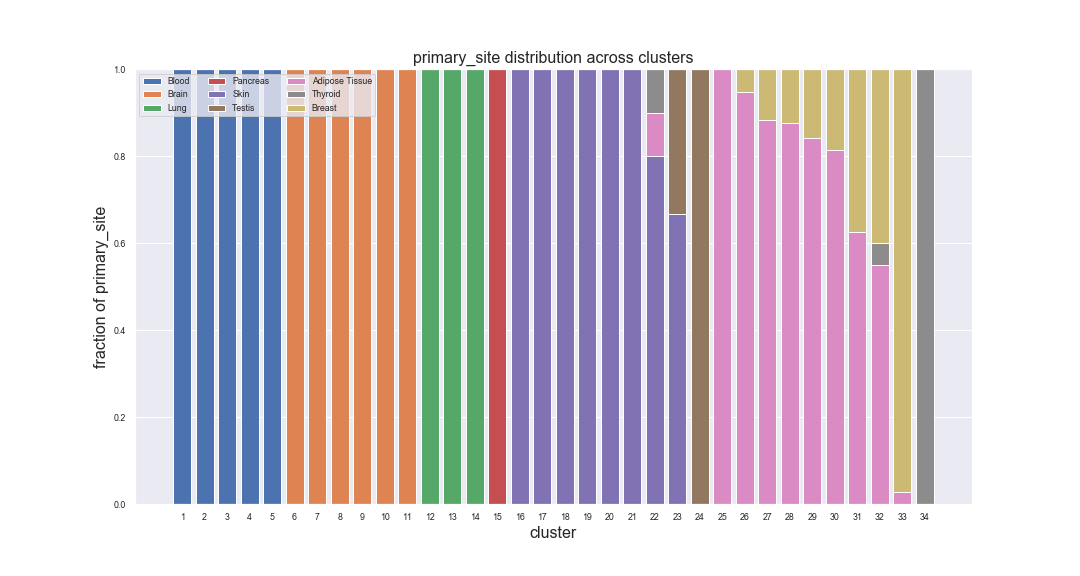
\includegraphics[width=0.9\linewidth]{pictures/topic/gtex/oversigma_10tissue/fraction_clustercomposition_l2_primary_site.png}
    \caption{Caption}
    \label{fig:topic/gtex/oversigma_10tissue/fraction_clustercomposition_l2_primary_site}
\end{figure}

\begin{figure}[htb!]
    \centering
    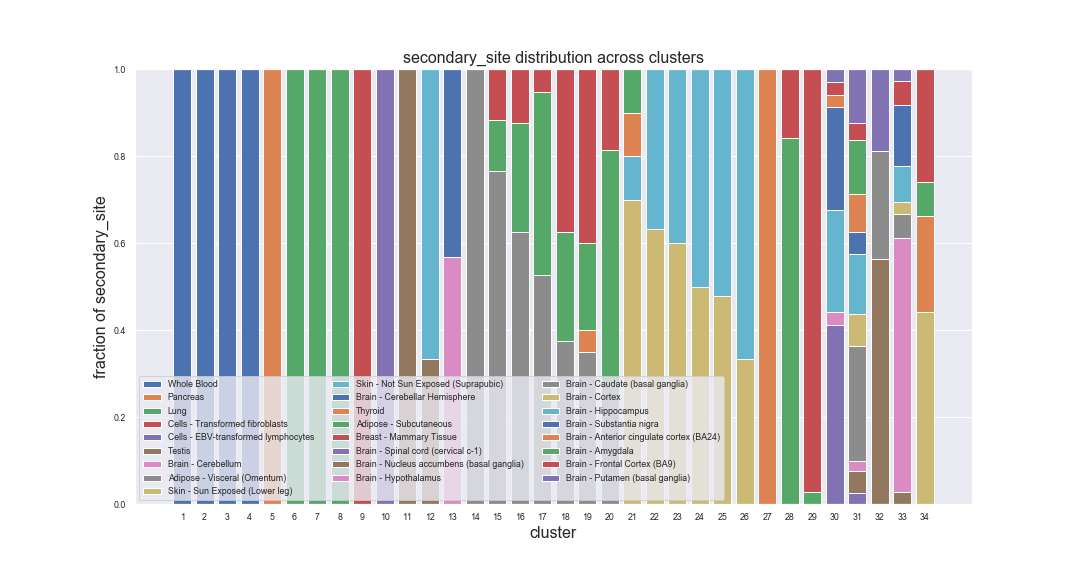
\includegraphics[width=0.9\linewidth]{pictures/topic/gtex/oversigma_10tissue/fraction_clustercomposition_l2_secondary_site.png}
    \caption{Caption}
    \label{fig:topic/gtex/oversigma_10tissue/fraction_clustercomposition_l2_secondary_site}
\end{figure}


Using as gene set ~\cite{Ardlie2015} enrichment test can be made \cite{Kuleshov2016}

Enrichment test are made once for each topic, starting from the layer with more genes per 
single topic. Test are made across multiple categories.

\section{Run on TCGA}

\section{Mixed runs}

\draft{hierarchical clustering}
\draft{This is better than LDA because...}

\chapter{Conclusions}\label{ch:conclusions}
Finally, this work demonstrates that RNA-sequencing datasets can be analysed from a component systems point of view.

Gene expression data show typical trends well-known, for example, in linguistics, moreover some interesting biological signatures were found. RNA-sequencing datasets have a great core of protein-coding genes that express everywhere, this is evident looking at $U$s or at Heaps' law. The presence of a power law distribution in the ranked abundances, the so-called Zipf's law is observed and characterize the distribution of genes expression data.

In the first part of this work a dataset (GTEx) containing samples from healthy tissues was analysed. One of the most interesting evidence was the presence of different Zipf's law if one considers each tissue independently. Very similar results were obtained considering TCGA, a dataset containing thousands of cancer samples.

The power law distributions and the similarities with what was found in linguistics encouraged to explore the possibility of using a topic model approach to reveal the hidden structure of these datasets. This approach, originally developed to classify text, was useful both to find clusters of samples that share some properties and to find the relation between genes and samples.

Many goals were achieved during the topic modelling analysis. The pipeline begins filtering the data and selecting highly variable genes, then this network is processed with hierarchical Stochastic Block Model algorithm, then clusters are analysed and enrichment tests are performed; in the meanwhile, an objective and a well-defined score is estimated. All the analysis confirmed that this approach is successful. Three different datasets were analysed and, in every case, the model performed well. What was found is that clusters contain samples that share some properties, in particular, the tissue they are related to; enrichment tests found tissue-related terms in the topics along with Gene Ontology terms. The relation between genes and samples is non-trivial and revealed a complex structure in gene expression data. Nevertheless, this structure is sufficient to discriminate between tissues.

In conclusion, topic modelling reveals itself as a useful approach to find the hidden structure of gene expression data. The prior analysis to select highly variables genes make it possible to run the algorithm faster without losing necessary information.

During this work the foundations have been laid for further analyses; for example, it should be interesting to study the variability of gene expression between tissues and between individual, ideally genes that change their behaviour inter different tissues and not intra the same tissue are more likely tissue-specific. Trying to remove the sampling effect from the data could be another interesting analysis, in particular reproducing~\cite{Grilli} on RNA-sequencing data could lead to the removal of sampling effects, here this was done just considering the sampling as a $CV^2$ boundary. Derive analytically the expression of the bound could be another goal. Use an innovation dynamic point of view to study the matrices discussed in this work can lead to other interesting results. Applying the model to single cell RNA-sequencing data, maybe from other kinds of animal, will present new challenges not present in bulk RNA-sequencing datasets considered here. Reproduce mouse data from~\cite{Scialdone2016} could be an interesting starting point. Maybe it worth to run the model on null data where just sampling is present and verify if there is some bias on the model due to the presence of the sampling.

The main future development of this work is indeed to run the model on a specific cancer tissue and find cancer subtypes, for instance, the breast or colon-rectal ones. Obtaining a hierarchy that at some level is able to identify cancer sub-types would be an ideal and great goal surely able to push further the human knowledge about cancer. 

%%APPENDIXES
\appendix
\addcontentsline{toc}{chapter}{Appendices}
\chapter{hierarchical stochastic block model}
The algorithm is called hierarchic Stochastic Block Model.

The first step of hSBM, as discussed in~\cite{peixoto2014efficient},
is to create a bipartite network $G$ with two kind of nodes: \textbf{words} and \textbf{documents}.
Every time a word $w$ is present in a document $d$ an edge $e_{wd}$ is created.
If a word count in the entire corpus is under a certain threshold, that word is ignored.
The aim is to find a partition $b\in\{b_i\}$ with $B=\left|\{b_i\}\right|$ blocks.

These kind of models are called \textit{generative models}: given the data the model
should generate a network $G$ with probability $P(G|\theta, b)$, where $b$ is
the partition and $\theta$ any additional parameter of the model.

Using well-known Bayes theorem one could estimate the probability that an
observed network is generated by partition $b$
\begin{equation}\label{eq:PbonG}
  P(b,\theta|G)=\frac{\Sigma_{\theta}P(G|b,\theta)\overbrace{P(b,\theta)}^{prior}}{\underbrace{P(G)}_{\Sigma_{\theta}P(G|\theta, b)P(\theta, b)}}
\end{equation}

defining the amount of information needed to describe the data as the description length
\begin{equation}\label{eq:descriptionlenght}
  \Sigma=-lnP(G|b,\theta)-lnP(b, \theta)
\end{equation}

the~\ref{eq:PbonG} can be written as $\frac{e^{-\Sigma}}{P(G)}$, so maximising
that is equivalent to minimise the description
length~\ref{eq:descriptionlenght}.
The probability of obteining a Graph from a set of paramenters is
$P(G|b,\theta)=\frac{1}{\Omega(A,\{n_r\})}$, where $\Omega(A,\{n_r\})$ is the
number of graph that is possible to generate with adiacence matrix $A$ and $n_r$
the counts of block partition $\{b_i\}$

In case of a weighted network the likelihood becomes $P(G,x|b,\theta)$, where $x$
are the weights.

\subsection{Algorithm}
First of all a $B\times B$ matrix is created. The entry $e_{rs}$ of this matrix
represents the number of links between nodes of group $r$ and nodes of group $s$,
with $r,s\in\{b_i\}$. At the beginning $B$ groups are formed at random and the initial $B$ is a hyper-parameter of the model.

\begin{figure}
  \centering
  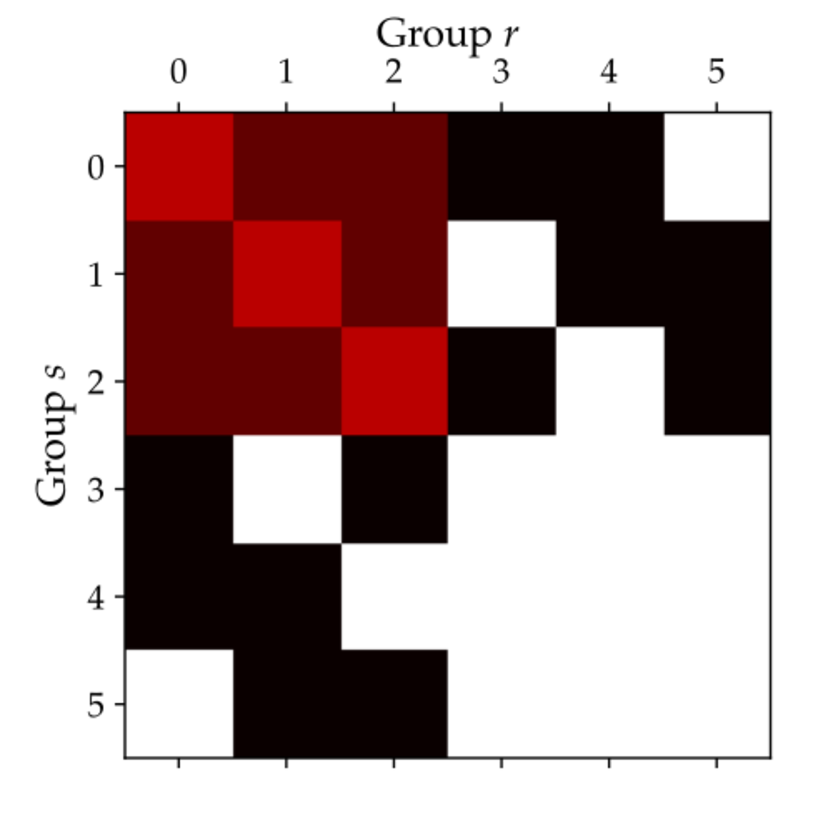
\includegraphics[width=0.3\linewidth]{pictures/topic/topic__pixioto_ers.pdf}
  \caption{Example of a edge's matrix from~\cite{peixoto_graph-tool_2014}}
    \label{fig:hsbm-ers}
\end{figure}

It is useful to define a traditional entropy:
\begin{equation}\label{eq:hSBMentropyt}
  S_t=\frac{1}{2}\Sigma_{r,s} n_rn_sH\left(\frac{e_{rs}}{n_rn_s}\right)
\end{equation}
where $n_{r}$ is the number of nodes in groups $r$, $e_{rs}$ is the
number of edges between nodes of group $r$ and nodes of group $s$, and
$H(x)=-xln(x)-(1-x)ln(1-x)$. This entropy is equivalent to the microcanonical
entropy of a system with ${\Omega(A,\{n_r\})}$ accessible states $S_t=Ln\Omega$.

The algorithm uses a Markov Chain MonteCarlo to minimise this entropy.
At each step a node changes block and the new configuration is accepted if $S$ is decreased.

Note that~\ref{eq:hSBMentropyt} can be corrected taking care of degree
distribution obtaining corrected entropy $S_c$
\begin{equation}
  S_c=-\Sigma_{r,s}\frac{e_{rs}}{2}-\Sigma_k
  N_kln(k!)-\frac{1}{2}\Sigma_{r,s}e_{rs}ln\left(\frac{e_{rs}}{e_re_s}\right)
\end{equation}

\paragraph{How to change group of a node?}
At each step according to~\cite{peixoto2014efficient} node $i$ can change group from $r$ to $s$ with a probability
\begin{equation}\label{eq:Prst}
  P(r\to s|t)=\frac{e_{ts}+\epsilon}{e_t+\epsilon B}
\end{equation}

\begin{figure}[htb!]
  \centering
  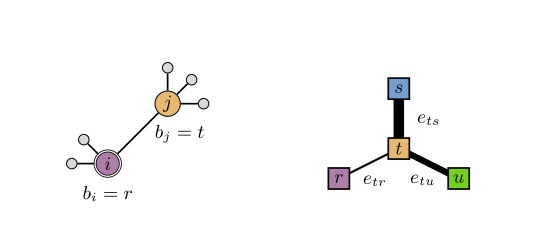
\includegraphics[width=0.9\linewidth]{pictures/topic/topic_pixioto_move.jpg}
  \caption{Left: Local neighbourhood of node $i$ belonging to block $r$, and a randomly chosen neighbour $j$ \
  belonging to block $t$. \
  Right: Block multigraph, indicating the number of edges between blocks, represented as the edge thickness. \
  In this example, the attempted move $bi \to s$ is made with a larger probability than either $bi \to u$\
   or $bi \to r$ (no movement), since $e_{ts}>e_{tu}$ and $e_{ts}>e_{tr}$.}
  \label{fig:topic_pixioto_move}
\end{figure}

where $j$ is a random neighbour of $i$: $j\in N_i$, $t\in\{b_j\}$ its block as defined in~\cite{peixoto2014efficient}.
$\epsilon$ is a parameter that according to~\cite{peixoto2017nonparametric} has no significant impact in the algorithm,
provided it is sufficiently small.

~\ref{eq:Prst} can be rewritten as \[P(r\to s|t)=(1-R_t)\frac{e_{ts}}{e_t}+\frac{R_t}{B}\]
defining $R_t=\frac{\epsilon B}{e_t + \epsilon B}$

This is done in four steps for each node $i$:
\begin{itemize}
  \item a node $j$ is chosen from $i$'s neighbours, the group of $j$ is called
  $t$
  \item a random group $s$ is selected
  \item move of node $i$ to group $s$ is accepted with probability $R_t$
  \item if $s$ is not accepted, a random edge $e$ is chosen from group $t$ and node $i$ is assigned to the endpoint of $e$ which is not in $t$
\end{itemize}
This steps mimate probability~\ref{eq:Prst}; note that for $\epsilon\to\infty$ this gives a uniform probability.

\paragraph{How many blocks $B$?}
Note that the number of blocks $B$ is a free parameter and must be inferred as described in~\cite{peixoto2017nonparametric}.
This implies a slight modification of the algorithm such that
it became possible to admit that a new group is created.
When a group $s$ is chosen, the algorithm can now accept a \textbf{new group} and~\ref{eq:Prst} became
\begin{equation}\label{eq:PrstB1}
  P(r\to s)=\Sigma_t P(t|i)\frac{e_{ts}+\epsilon}{e_t+\epsilon (B+1)}
\end{equation}
Being $P(t|i)=\Sigma_j\frac{A_{ij}\delta(b_j, t)}{k_i}$ the fraction of neighbours of $i$ belonging to group $t$, $e_t$ the number of edges in group $t$,
$k_i$ the degree, and $b_j$ groups.

Using this modification it is now possible to add new groups and $B$ is no longer a parameter.

\paragraph{How to find hierarchic layers?}
After the algorithm is run, one may would to add a new hierarchic level, this is done considering the $B$ groups as nodes and repeating the process.
As done before a matrix of edges like~\ref{fig:hsbm-ers} is created, where edges
are considered between groups of the previous layer.

\begin{figure}
  \centering
  \includegraphics[width=0.6\linewidth]{pictures/topic/topic_peixioto_hierarchic.jpg}
  \caption{Hierachical structure}
  \label{fig:topic_peixioto_hierarchic}
\end{figure}

The posterior probability became
\begin{equation}\label{eq:posteriorL}
  P(\{b_l\}|A)=\frac{P(A|\{b_l\})P(\{b_l\})}{P(A)}=\prod_l^L P(b_l|e_l,b_{l-1})
\end{equation}
Where $l=0\dots L$ is the layer, $A$ the adiacence matrix, $b_i$ blocks. Note that $e_0=A$ and $B_L=1$.
Maximising~\ref{eq:posteriorL} gives the correct number of layers.

Adding a layer is done in 3 steps described in~\cite{peixoto2014hierarchic}:
\begin{itemize}
  \item[Resize] find $B_l\in[B_{l-1},B_{l+1}]$ by bisection
  \item[Insert] a layer l
  \item[Delete] $l$ and linking nodes from layer $l-1$ directly to groups of layer
  $l+1$
\end{itemize}
One marks initially all levels as not done and starts at the top level $l = L$~\cite{peixoto2014hierarchic}.
For the current level $l$, if it is marked done it is skipped and one moves to the level $l-1$.
Otherwise, all three moves are attempted. If any of the moves succeeds in decreasing the description length $\Sigma$~\ref{eq:descriptionlenght},
one marks the levels $l-1$ and $l+1$ (if they exist) as not done, the level $l$ as done, and one proceeds (if possible)
to the upper level $l+1$, and repeats the procedure.
If no improvement is possible, the level $l$ is marked as done and one proceeds to the lower level $l-1$.
If the lowest level $l=0$ is reached and cannot be improved, the algorithm ends.


%%done by eristic agglomerative

\paragraph{Overlapping partitions}
As described in~\cite{peixoto2015model} one of the advantages of this approach
is that it is possible to let a node belonging to multiple groups.
In this case $b_i$ becomes $\vec{b_i}$, with component $b_{ir}=1$ if node $i$ is in
group $r$, $0$ otherwise. The number of $1$s in vector $\vec{b_i}$ is called
$d_i=|\vec{b_i}|$.

The probability of having a graph $G$ being generated from an adiacence matrix
$A$ and a partition $\{\vec{b_i}\}$ is \[P(G|A,\{\vec{b_i}\})=\frac{1}{\Omega}\]
if $\Omega$ is the number of possible graphs. Entropy~\ref{eq:hSBMentropyt} is
$S_t=Ln\Omega$. This corresponds to an augmented graph generated via a
non overlapping block model with $N'=\Sigma_r n_r>N$ nodes and the same
adiacence matrix $A$.

First of all, it is necessary to sample the distribution of mixture sizes
$P(\{n_d\})$ where $n_d$ is the number of nodes which mixture has got size $d$, $n_d\in[0,N]$ and $d\in[0,D]$ (typically $D=B$
and in the non-overlapping case $D=1$), this is done by sampling uniformly from
\[P(\{n_d\}|B)=\left(\binom{D}{N}\right)^{-1}\] which is probability of having $n$ nodes whose mixture has size $d$.
$\left(\binom{B}{N}\right)$ is the number of histograms with
area $N$ and $B$ distiguishable bins. $B-1$ can be used instead of $B$ to avoid node with no group, in this case $d\in[1,B]$.

Given the mixture sizes, the distribution of node membership
is sampled from \[P(\{d_i\}|\{n_d\})=\frac{\prod_{d} n_d!}{N!}\].

At this point for each set of nodes with $d_i=d$ it is necessary to sample $n_{\vec{b}}$; the number of nodes
with a particular mixture $\vec{b}$.
It is sampled from
\begin{equation}
  P(\{n_{\vec{b}}\}_d|n_d)=\left(\binom{\binom{D}{d}}{n_d}\right)^{-1}
\end{equation}

Next all mixtures $\vec{b_i}$ of size $d$ must be sampled, they are given by
\begin{equation}
  P(\{\vec{b_i}\}_d|\{n_{\vec{b}}\}_d)=\frac{\prod_{|\vec{b_i}|=d} n_b!}{n_d!}
\end{equation}

the global posterior as defined in~\cite{peixoto2015model} is
\begin{equation}
  P(\{\vec{b_i}\}|B)=\left[\prod_{d=1}^B  P(\{\vec{b_i}\}_d|\{n_{\vec{b}}\}_d) P(\{n_{\vec{b}}\}_d|n_d)\right]P({d_i}|{n_d})P(n_d|B)
\end{equation}

At this time it is necessary to obtain the distribution of the edges between
mixtures. Defined $e_r=\Sigma_s e_{rs}$ the number of half-edges labeled $r$,
$m_r=\Sigma_{\vec{b}} b_r$ the number of mixtures containing group $r$ the
algorithm samples the probability distribution of the edges count
\[P(\{e_{\vec{b}}\}|\{\vec{b_i}\}, A)=\prod_r\left(\binom{m_r}{e_r}\right)^{-1}\] and the
labeled degree sequence $\{\vec{k_i}\}$ from
\[P(\{\vec{k_i}\}_{\vec{b}}|\{e_{\vec{b}}\}, \{\vec{b_i}\})=\frac{\prod_k n_k^{\vec{b}}!}{n_{\vec{b}}!}\]


\paragraph{Word documents separation}
Following what is done in~\cite{gerlach2018network}, the probability of a group $P(b_l)$ at a certain level $l$ is intended as the disjoint probability of
group of words and group of documents.
\begin{equation}
  P(b_l)=P_w(b_l^w)P_d(b_l^d)
\end{equation}

Doing this let words and documents be separated by construction.
Considering the process described above if two nodes are not connected at the beginning it is impossible
that they end up in the same block.
It is easly verified in~\cite{peixoto2014efficient} that this property is
preserved and fully reflected in the final block structure.

\subsection{Topics}

Once the model is run it is possible to extimate the probability distribution of words inside a topic
\[P(w|t_w)=\frac{\text{\# of edges on $w$ to $t_w$}}{\text{\# of edges on $t_w$}}\]
and the topic distribution inside a document
\[P(t_w|d)=\frac{\text{\# of edges on $d$ from $t_w$}}{\text{\# of edges on $d$}}\]
In case of overlapping partitions it is possible to extimate the presence of a
word in a topic
\[P(t_w|w)=\frac{\text{\# of edges on $w$ to $t_w$}}{\text{\# of edges on $w$}}\]
or the presence of a document in a cluster
\[P(t_d|d)=\frac{\text{\# of edges on $d$ to $t_d$}}{\text{\# of edges on $d$}}\]

\subsection{LDA}
As in ~\cite{Zhou2016}

\begin{equation}\label{eq:lda}
  P(w, z,\beta, \theta| \alpha, \eta)=\prod_n^{N_d} P(w|z,\beta)P(z|\theta)\prod_k^KP(\beta|\eta)\prod_d^N P(\theta | \alpha)
\end{equation}

\begin{figure}
  \centering
  \includegraphics[width=0.5\linewidth]{pictures/topic/LDA.jpeg}
  \label{fig:LDA}
  \caption{LAD scheme}
\end{figure}

where

\begin{itemize}
  \item $N$ number of documents
  \item $K$ number of topics
  \item $w$ words
  \item $N_d$ number of words in document d
  \item $\eta$ and $\alpha$ are parameters of the model
\end{itemize}

in~\ref{eq:lda} $P(\theta | \alpha)$ and $P(\beta|\eta)$ are Dirichlet distributions

the outputs are the topic distribution in documents $P(z|d)$ and the word distribution in topics $P(w|z)$


\chapter{Homogeneity, completeness and V-measure}\label{app:vmeasure}
Using algorithms that are unsupervised, but with a ground truth available it is useful to define some metrics.

The homogeneity
\begin{equation}
    h=1-\frac{h(C|K)}{H(C)}
\end{equation}
defining the entropy
\begin{equation}
    H(C|K)=\sum_{c\in \mathrm{model labels},\\ k \in \mathrm{clusters}}\frac{n_{c k}}{N}Log\left(\frac{n_{c k}}{n_k}\right)
\end{equation}
where $n_{c k}$ is the number of nodes of type $c$ in cluster $k$, $N$ the number of nodes and $n_k$ the number of nodes in cluster $k$. It is evident that if all nodes inside cluster $k$ are of the same type $c$ $n_{c k}=n_{k}$, $H(C|K)=0$ and $h=1$, it is actually a complete homogeneous situation.
The completeness:
\begin{equation}
    c=1-\frac{h(K|C)}{H(K)},
\end{equation}
$H(K|C)$ is defined in the same way as $H(C|K)$. Completeness measures if all nodes of the same type are in the same cluster.
Ideally one wants a model which output is both homogeneous and complete. So it is possible to define the V-measure~\cite{rosenberg2007v}, which is the harmonic average of the two:
\begin{equation}
    2\frac{h c}{h + c}.
\end{equation}

The product $h c$ is equal to
\begin{equation}
    \frac{(H(C)-H(C|K))(H(K)-H(K|C))}{H(K) H(C)},
\end{equation}
the sum $h + c$ is
\begin{equation}
    \frac{H(K)(H(C)-H(C|K))+H(C)(H(K)-H(K|C))}{H(K) H(C)}.
\end{equation}
Expressing the conditional entropy 
\[
H(K|C)=\sum_{k c} P(k,c)Log(P(k|c))
\\=\sum_{k c} P(k,c)Log\left(\frac{P(k,c)}{P(c)}\right)
\\=H(K,C) - H(C)
\]
in terms of the conjunct entropy $H(K,C)$ which is symmetric by exchanges of $C$ and $K$
\[
H(K,C)=H(K|C) + H(C) = H(C|K) + H(K) = H(C,K)
\]
it is easy to verify that 
\[
H(C) - H(C|K) = H(K) - H(K|C) 
\]
so
\[
h c = \frac{(H(C)-H(C|K))^2}{H(K) H(C)}
\]
and
\[
h + c = \frac{(H(C)-H(C|K))(H(K)+H(C))}{H(K) H(C)}.
\]
The harmonic average $2\frac{h c}{h + c}$ becomes
\[
2\frac{H(C)-H(C|K)}{H(K)+H(C)}=2\frac{H(C)+H(K)-H(K,C)}{H(K)+H(C)}=2\frac{MI(C,K)}{H(K)+H(C)}
\]
which is called V-measure and is actually the mutual information between $P(C)$ and $P(K)$ normalised to $1$ by the term $H(C)+H(K)$. In fact if $P(C)=P(K)$ $H(K,C)=H(K)=H(C)$ and the measure is $1$, if $P(C)$ and $P(K)$ are completely independent $H(K,C)=H(K)+H(C)$ and the measure is $0$.


%%%% TAIL OF THE DOCUMENT
\backmatter
%list of figures
\listoffigures
\clearemptydoublepage
%list of tables
\listoftables
\clearemptydoublepage

%bibliography
\addcontentsline{toc}{chapter}{Bibliography}
\bibliography{bibliography/bibThesis}
\bibliographystyle{ieeetr}
\clearemptydoublepage

\addcontentsline{toc}{chapter}{Acknowledgements}
\chapter*{Acknowledgements}
\draft{Ringrazio bla bla bla...}

L'intero gruppo \url{http://personalpages.to.infn.it/~caselle/BioPhys/BioPhys.html}

\end{document}
